\PassOptionsToPackage{unicode=true}{hyperref} % options for packages loaded elsewhere
\PassOptionsToPackage{hyphens}{url}
\documentclass[14pt,ignorenonframetext,aspectratio=169]{beamer}
\IfFileExists{pgfpages.sty}{\usepackage{pgfpages}}{}
\setbeamertemplate{caption}[numbered]
\setbeamertemplate{caption label separator}{: }
\setbeamercolor{caption name}{fg=normal text.fg}
\beamertemplatenavigationsymbolsempty
\usepackage{lmodern}
\usepackage{amssymb,amsmath}
\usepackage{ifxetex,ifluatex}
\usepackage{fixltx2e} % provides \textsubscript
\ifnum 0\ifxetex 1\fi\ifluatex 1\fi=0 % if pdftex
  \usepackage[T1]{fontenc}
  \usepackage[utf8]{inputenc}
\else % if luatex or xelatex
  \ifxetex
    \usepackage{mathspec}
  \else
    \usepackage{fontspec}
\fi
\defaultfontfeatures{Ligatures=TeX,Scale=MatchLowercase}







\fi

  \usetheme[]{monash}

  \usecolortheme{monashwhite}


% A default size of 24 is set in beamerthememonash.sty

% Title page
\setbeamertemplate{title page}
{\placefig{-0.01}{-0.01}{width=1.01\paperwidth,height=1.01\paperheight}{title16x9.png}
\begin{textblock}{7.5}(1,2.8)\usebeamerfont{title}
{\color{burntorange}\raggedright\par\inserttitle}
\end{textblock}
\begin{textblock}{7.5}(1,7)
{\color{burntorange}\raggedright{\insertauthor}\mbox{}\\[0.2cm]
\insertdate}
\end{textblock}}




% use upquote if available, for straight quotes in verbatim environments
\IfFileExists{upquote.sty}{\usepackage{upquote}}{}
% use microtype if available
\IfFileExists{microtype.sty}{%
  \usepackage{microtype}
  \UseMicrotypeSet[protrusion]{basicmath} % disable protrusion for tt fonts
}{}


\newif\ifbibliography


\hypersetup{
      pdftitle={ETC3550/ETC5550 Applied~forecasting},
        pdfauthor={Ch2. Time series graphics},
          pdfborder={0 0 0},
    breaklinks=true}
%\urlstyle{same}  % Use monospace font for urls




  \usepackage{color}
  \usepackage{fancyvrb}
  \newcommand{\VerbBar}{|}
  \newcommand{\VERB}{\Verb[commandchars=\\\{\}]}
  \DefineVerbatimEnvironment{Highlighting}{Verbatim}{commandchars=\\\{\}}
  % Add ',fontsize=\small' for more characters per line
  \usepackage{framed}
  \definecolor{shadecolor}{RGB}{248,248,248}
  \newenvironment{Shaded}{\begin{snugshade}}{\end{snugshade}}
  \newcommand{\AlertTok}[1]{\textcolor[rgb]{0.94,0.16,0.16}{#1}}
  \newcommand{\AnnotationTok}[1]{\textcolor[rgb]{0.56,0.35,0.01}{\textbf{\textit{#1}}}}
  \newcommand{\AttributeTok}[1]{\textcolor[rgb]{0.77,0.63,0.00}{#1}}
  \newcommand{\BaseNTok}[1]{\textcolor[rgb]{0.00,0.00,0.81}{#1}}
  \newcommand{\BuiltInTok}[1]{#1}
  \newcommand{\CharTok}[1]{\textcolor[rgb]{0.31,0.60,0.02}{#1}}
  \newcommand{\CommentTok}[1]{\textcolor[rgb]{0.56,0.35,0.01}{\textit{#1}}}
  \newcommand{\CommentVarTok}[1]{\textcolor[rgb]{0.56,0.35,0.01}{\textbf{\textit{#1}}}}
  \newcommand{\ConstantTok}[1]{\textcolor[rgb]{0.00,0.00,0.00}{#1}}
  \newcommand{\ControlFlowTok}[1]{\textcolor[rgb]{0.13,0.29,0.53}{\textbf{#1}}}
  \newcommand{\DataTypeTok}[1]{\textcolor[rgb]{0.13,0.29,0.53}{#1}}
  \newcommand{\DecValTok}[1]{\textcolor[rgb]{0.00,0.00,0.81}{#1}}
  \newcommand{\DocumentationTok}[1]{\textcolor[rgb]{0.56,0.35,0.01}{\textbf{\textit{#1}}}}
  \newcommand{\ErrorTok}[1]{\textcolor[rgb]{0.64,0.00,0.00}{\textbf{#1}}}
  \newcommand{\ExtensionTok}[1]{#1}
  \newcommand{\FloatTok}[1]{\textcolor[rgb]{0.00,0.00,0.81}{#1}}
  \newcommand{\FunctionTok}[1]{\textcolor[rgb]{0.00,0.00,0.00}{#1}}
  \newcommand{\ImportTok}[1]{#1}
  \newcommand{\InformationTok}[1]{\textcolor[rgb]{0.56,0.35,0.01}{\textbf{\textit{#1}}}}
  \newcommand{\KeywordTok}[1]{\textcolor[rgb]{0.13,0.29,0.53}{\textbf{#1}}}
  \newcommand{\NormalTok}[1]{#1}
  \newcommand{\OperatorTok}[1]{\textcolor[rgb]{0.81,0.36,0.00}{\textbf{#1}}}
  \newcommand{\OtherTok}[1]{\textcolor[rgb]{0.56,0.35,0.01}{#1}}
  \newcommand{\PreprocessorTok}[1]{\textcolor[rgb]{0.56,0.35,0.01}{\textit{#1}}}
  \newcommand{\RegionMarkerTok}[1]{#1}
  \newcommand{\SpecialCharTok}[1]{\textcolor[rgb]{0.00,0.00,0.00}{#1}}
  \newcommand{\SpecialStringTok}[1]{\textcolor[rgb]{0.31,0.60,0.02}{#1}}
  \newcommand{\StringTok}[1]{\textcolor[rgb]{0.31,0.60,0.02}{#1}}
  \newcommand{\VariableTok}[1]{\textcolor[rgb]{0.00,0.00,0.00}{#1}}
  \newcommand{\VerbatimStringTok}[1]{\textcolor[rgb]{0.31,0.60,0.02}{#1}}
  \newcommand{\WarningTok}[1]{\textcolor[rgb]{0.56,0.35,0.01}{\textbf{\textit{#1}}}}

  \usepackage{longtable,booktabs}
  \usepackage{caption}
  % These lines are needed to make table captions work with longtable:
  \makeatletter
  \def\fnum@table{\tablename~\thetable}
  \makeatother

  \usepackage{graphicx,grffile}
  \makeatletter
  \def\maxwidth{\ifdim\Gin@nat@width>\linewidth\linewidth\else\Gin@nat@width\fi}
  \def\maxheight{\ifdim\Gin@nat@height>\textheight0.8\textheight\else\Gin@nat@height\fi}
  \makeatother
  % Scale images if necessary, so that they will not overflow the page
  % margins by default, and it is still possible to overwrite the defaults
  % using explicit options in \includegraphics[width, height, ...]{}
  \setkeys{Gin}{width=\maxwidth,height=\maxheight,keepaspectratio}

% Prevent slide breaks in the middle of a paragraph:
\widowpenalties 1 10000
\raggedbottom

  \AtBeginPart{
    \let\insertpartnumber\relax
    \let\partname\relax
    \frame{\partpage}
  }
  \AtBeginSection{
    \ifbibliography
    \else
      \let\insertsectionnumber\relax
      \let\sectionname\relax
      \frame{\sectionpage}
    \fi
  }
  \AtBeginSubsection{
    \let\insertsubsectionnumber\relax
    \let\subsectionname\relax
    \frame{\subsectionpage}
  }



\setlength{\parindent}{0pt}
\setlength{\parskip}{6pt plus 2pt minus 1pt}
\setlength{\emergencystretch}{3em}  % prevent overfull lines
\providecommand{\tightlist}{%
  \setlength{\itemsep}{0pt}\setlength{\parskip}{0pt}}

  \setcounter{secnumdepth}{0}


%% Monash overrides
\AtBeginSection[]{
   \frame<beamer>{
   \frametitle{Outline}\vspace*{0.2cm}
   
   \tableofcontents[currentsection,hideallsubsections]
  }}

% Redefine shaded environment if it exists (to ensure text is black)
\ifcsname Shaded\endcsname
  \definecolor{shadecolor}{RGB}{225,225,225}
  \renewenvironment{Shaded}{\color{black}\begin{snugshade}\color{black}}{\end{snugshade}}
\fi
%%

  % Packages
  \usepackage{bm,booktabs,tabularx}
  \usepackage{animate,soul}
  \DeclareUnicodeCharacter{03BC}{$\mu$}
  \usepackage{fontawesome}

  % Figures
  \graphicspath{{figs/}}

  % Fonts
  \fontsize{13}{15}\sf
  \usepackage[scale=0.85]{sourcecodepro}
  \DisableLigatures{encoding = T1, family = tt*}
  \setbeamerfont{title}{series=\bfseries,parent=structure,size=\fontsize{18}{20}}
  \ifcsname Shaded\endcsname
    \definecolor{shadecolor}{RGB}{225,225,225}
    \renewenvironment{Shaded}{\color{black}\fontsize{10}{10}\sf\begin{snugshade}\color{black}}{\end{snugshade}}
  \fi

  % Colors
  \setbeamercolor{description item}{fg=Orange}
  \definecolor{MonashBlue}{RGB}{69,88,94}
  \definecolor{burntorange}{rgb}{0.8, 0.33, 0.0}

  % tikz diagrams
  \usepackage{tikz}
  \usetikzlibrary{shapes,arrows}
  \tikzstyle{decision} = [diamond, draw, fill=blue!20,
      text width=4.5em, text badly centered, node distance=4cm, inner sep=0pt]
  \tikzstyle{block} = [rectangle, draw, fill=blue!20,
      text width=5cm, text centered, rounded corners, minimum height=4em]
  \tikzstyle{line} = [draw, thick, -latex']
  %\tikzstyle{line} = [->,thi
  \tikzstyle{cloud} = [draw, ellipse,fill=red!20, node distance=3cm,
      minimum height=2em, text centered]
  \tikzstyle{connector} = [->,thick]

  % gt dependencies
  \usepackage{longtable,caption,setspace}
  \captionsetup{font={small,stretch=0.80}}

  % My definitions

  \def\E{\text{E}}
  \def\V{\text{Var}}
  \def\up#1{\raisebox{-0.3cm}{#1}}
  \def\pred#1#2#3{\hat{#1}_{#2|#3}}
  \def\damped{$_\text{d}$}
  \def\h+{h_{m}^{+}}
  \def\str#1{\rlap{#1}\textcolor{red}{\rule{1cm}{0.1cm}}}

  \def\forecast{\begin{alertblock}{}\fontsize{10}{11}\sf
  A forecast is an estimate of the probabilities of possible futures.
  \end{alertblock}}

  \def\simfutures{\begin{textblock}{2.7}(13,7.7)
  \begin{block}{}\fontsize{10}{11}\sf
  Simulated futures from an ETS model
  \end{block}\end{textblock}}

  \def\fullwidth#1{\centerline{\includegraphics[height=27.1cm,width=16cm,keepaspectratio=true]{#1}}}
  \def\fullheight#1{\centerline{\includegraphics[height=7.65cm,width=25cm,keepaspectratio=true]{#1}}}
  \def\full#1{\centerline{\includegraphics[height=7.7cm,width=15cm,keepaspectratio=true]{#1}}}

  % Title page graphic
    \titlegraphic{
      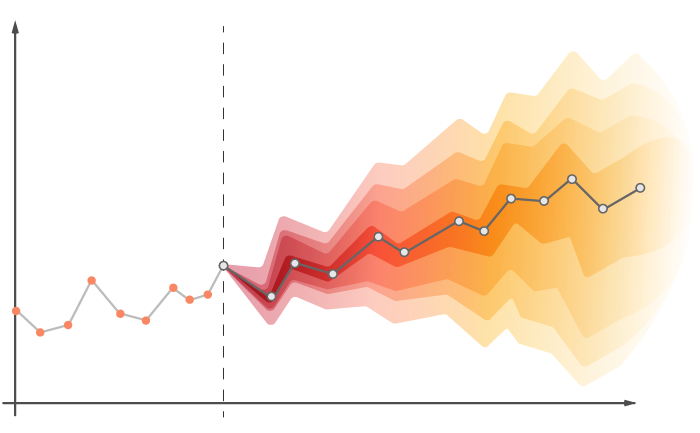
\includegraphics[height=1.5in]{./Images/probabilistic-forecasting-graph.png} \vspace{1in}
    }
    
    % Vanderbilt color scheme
    \usepackage{xcolor}
    \definecolor{gold}{RGB}{207,174,112}  % gold
    \definecolor{black}{RGB}{10,10,10} % black
    \definecolor{white}{RGB}{255,255,255} % white
    \setbeamercolor{title}{fg = gold}
    \setbeamercolor{title}{bg = black}
    \setbeamercolor{normal text}{fg = black}
    \setbeamercolor{frametitle}{fg = gold}
    \setbeamercolor{frametitle}{bg = black}
    \setbeamercolor{structure}{fg = gold}
    \setbeamercolor{structure}{bg = black}
    \setbeamercolor{item}{fg = black}
    
    % Other stuff
    \usepackage{amssymb}
    \usepackage{ragged2e}
    \usepackage{multicol}
    \usepackage{mwe}
    \usepackage{textpos}
    
    % Default setup
    \usepackage[sfdefault]{cabin}
    \usepackage{hyperref}
    %\hypersetup{
    %  colorlinks = true,
    %  allcolors = blue
    %}
    \usepackage{float, placeins}
    \usepackage{booktabs}
    
    % Additional packages
    \usepackage[edges]{forest}
    
    % tikz equation packages
    \usepackage{tikz}
    \usetikzlibrary{backgrounds}
    \usetikzlibrary{tikzmark}
    \usetikzlibrary{calc}
    \usetikzlibrary{arrows,shapes,positioning,shadows,trees,mindmap}
    \usetikzlibrary{arrows.meta}
    \colorlet{linecol}{black!75}
    \usepackage{xkcdcolors} % xkcd colors

    % Basic equation packages
    \usepackage{amsmath}
    \usepackage{amsthm}
    \usepackage{amssymb}
    \usepackage{mathtools}
    \usepackage{nccmath}
    \usepackage{wrapfig}
    \usepackage{comment}
    \usepackage{blindtext}
    \usepackage{graphicx}
    \usepackage{xspace}
    \usepackage{array}
    \usepackage{ragged2e}
    \newcolumntype{P}[1]{>{\RaggedRight\hspace{0pt}}p{#1}}
    \newcolumntype{X}[1]{>{\RaggedRight\hspace*{0pt}}p{#1}}
    \DeclarePairedDelimiter{\norm}{\lVert}{\rVert}


    % Color packages
    \usepackage{xcolor}
    \usepackage{tcolorbox}
    \newcommand{\highlight}[2]{\colorbox{#1!30}{$\displaystyle #2$}}
    \newcommand{\highlightdark}[2]{\colorbox{#1!50}{$\displaystyle #2$}}
    \renewcommand{\highlight}[2]{\colorbox{#1!30}{#2}}
    \renewcommand{\highlightdark}[2]{\colorbox{#1!50}{#2}}
    
    % Define colors
    \definecolor{red}{HTML}{F03D2D}
    \definecolor{skyblue}{HTML}{90DDF0}
    \definecolor{green}{HTML}{C8D96F}
    \definecolor{orange}{HTML}{EF8A17}
    \definecolor{yellow}{HTML}{F5C900}
    \definecolor{purple}{HTML}{BA42C0}
    \definecolor{teal}{HTML}{17BEBB}
    \definecolor{greyblue}{HTML}{9BAFD9}


  \title[]{ETC3550/ETC5550 Applied~forecasting}


  \author[
        Ch2. Time series graphics
    ]{Ch2. Time series graphics}


\date[
      OTexts.org/fpp3/
  ]{
      OTexts.org/fpp3/
        }

\begin{document}

% Hide progress bar and footline on titlepage
  \begin{frame}[plain]
  \titlepage
  \end{frame}


   \frame<beamer>{
   \frametitle{Outline}\vspace*{0.2cm}
   
   \tableofcontents[hideallsubsections]
  }

\hypertarget{time-series-in-r}{%
\section{Time series in R}\label{time-series-in-r}}

\begin{frame}[fragile]{\texttt{tsibble} objects}
\protect\hypertarget{tsibble-objects}{}
\fontsize{10}{11.2}\sf

\begin{Shaded}
\begin{Highlighting}[]
\NormalTok{global\_economy}
\end{Highlighting}
\end{Shaded}

\begin{verbatim}
## # A tsibble: 15,150 x 6 [1Y]
## # Key:       Country [263]
##     Year Country             GDP Imports Exports Population
##    <dbl> <fct>             <dbl>   <dbl>   <dbl>      <dbl>
##  1  1960 Afghanistan  537777811.    7.02    4.13    8996351
##  2  1961 Afghanistan  548888896.    8.10    4.45    9166764
##  3  1962 Afghanistan  546666678.    9.35    4.88    9345868
##  4  1963 Afghanistan  751111191.   16.9     9.17    9533954
##  5  1964 Afghanistan  800000044.   18.1     8.89    9731361
##  6  1965 Afghanistan 1006666638.   21.4    11.3     9938414
##  7  1966 Afghanistan 1399999967.   18.6     8.57   10152331
##  8  1967 Afghanistan 1673333418.   14.2     6.77   10372630
##  9  1968 Afghanistan 1373333367.   15.2     8.90   10604346
## 10  1969 Afghanistan 1408888922.   15.0    10.1    10854428
## # ... with 15,140 more rows
## # i Use `print(n = ...)` to see more rows
\end{verbatim}

\only<2->{\begin{textblock}{.75}(2.15,3.7)
\begin{alertblock}{}\fontsize{10}{10}\sf Index\phantom{dg}\end{alertblock}
\end{textblock}}
\only<3->{\begin{textblock}{1.6}(3.28,3.7)
\begin{alertblock}{}\fontsize{10}{10}\sf Key\phantom{dg}\end{alertblock}
\end{textblock}}
\only<4>{\begin{textblock}{6.7}(5.5,3.7)
\begin{alertblock}{}\fontsize{10}{10}\sf Measured variables\phantom{dg}\end{alertblock}
\end{textblock}}
\end{frame}

\begin{frame}[fragile]{\texttt{tsibble} objects}
\protect\hypertarget{tsibble-objects-1}{}
\fontsize{10}{11.3}\sf

\begin{Shaded}
\begin{Highlighting}[]
\NormalTok{tourism}
\end{Highlighting}
\end{Shaded}

\begin{verbatim}
## # A tsibble: 24,320 x 5 [1Q]
## # Key:       Region, State, Purpose [304]
##    Quarter Region   State Purpose  Trips
##      <qtr> <chr>    <chr> <chr>    <dbl>
##  1 1998 Q1 Adelaide SA    Business  135.
##  2 1998 Q2 Adelaide SA    Business  110.
##  3 1998 Q3 Adelaide SA    Business  166.
##  4 1998 Q4 Adelaide SA    Business  127.
##  5 1999 Q1 Adelaide SA    Business  137.
##  6 1999 Q2 Adelaide SA    Business  200.
##  7 1999 Q3 Adelaide SA    Business  169.
##  8 1999 Q4 Adelaide SA    Business  134.
##  9 2000 Q1 Adelaide SA    Business  154.
## 10 2000 Q2 Adelaide SA    Business  169.
## # ... with 24,310 more rows
## # i Use `print(n = ...)` to see more rows
\end{verbatim}

\only<2->{\begin{textblock}{1.1}(2.1,3.65)
\begin{alertblock}{}\fontsize{10}{10}\sf Index\phantom{dg}\end{alertblock}
\end{textblock}}
\only<3->{\begin{textblock}{3.9}(3.65,3.65)
\begin{alertblock}{}\fontsize{10}{10}\sf Keys\phantom{dg}\end{alertblock}
\end{textblock}}
\only<4-5>{\begin{textblock}{1.5}(7.95,3.65)
\begin{alertblock}{}\fontsize{10}{10}\sf Measure\phantom{dg}\end{alertblock}
\end{textblock}}

\only<5>{\begin{textblock}{3}(9,5)
\begin{block}{}\fontsize{10}{10}\sf Domestic visitor nights in thousands by state/region and purpose.\phantom{dg}\end{block}
\end{textblock}}
\end{frame}

\begin{frame}[fragile]{\texttt{tsibble} objects}
\protect\hypertarget{tsibble-objects-2}{}
\begin{itemize}
\item
  A \texttt{tsibble} allows storage and manipulation of multiple time
  series in R.
\item
  It contains:

  \begin{itemize}
  \tightlist
  \item
    An index: time information about the observation
  \item
    Measured variable(s): numbers of interest
  \item
    Key variable(s): optional unique identifiers for each series
  \end{itemize}
\item
  It works with tidyverse functions.
\end{itemize}
\end{frame}

\begin{frame}[fragile]{The \texttt{tsibble} index}
\protect\hypertarget{the-tsibble-index}{}
\begin{block}{Example}
\protect\hypertarget{example}{}
\fontsize{11}{12}\sf

\begin{Shaded}
\begin{Highlighting}[]
\NormalTok{mydata }\OtherTok{\textless{}{-}} \FunctionTok{tsibble}\NormalTok{(}
    \AttributeTok{year =} \DecValTok{2012}\SpecialCharTok{:}\DecValTok{2016}\NormalTok{,}
    \AttributeTok{y =} \FunctionTok{c}\NormalTok{(}\DecValTok{123}\NormalTok{, }\DecValTok{39}\NormalTok{, }\DecValTok{78}\NormalTok{, }\DecValTok{52}\NormalTok{, }\DecValTok{110}\NormalTok{),}
    \AttributeTok{index =}\NormalTok{ year}
\NormalTok{)}
\NormalTok{mydata}
\end{Highlighting}
\end{Shaded}

\begin{verbatim}
## # A tsibble: 5 x 2 [1Y]
##    year     y
##   <int> <dbl>
## 1  2012   123
## 2  2013    39
## 3  2014    78
## 4  2015    52
## 5  2016   110
\end{verbatim}
\end{block}
\end{frame}

\begin{frame}[fragile]{The \texttt{tsibble} index}
\protect\hypertarget{the-tsibble-index-1}{}
\begin{block}{Example}
\protect\hypertarget{example-1}{}
\fontsize{11}{12}\sf

\begin{Shaded}
\begin{Highlighting}[]
\NormalTok{mydata }\OtherTok{\textless{}{-}} \FunctionTok{tibble}\NormalTok{(}
    \AttributeTok{year =} \DecValTok{2012}\SpecialCharTok{:}\DecValTok{2016}\NormalTok{,}
    \AttributeTok{y =} \FunctionTok{c}\NormalTok{(}\DecValTok{123}\NormalTok{, }\DecValTok{39}\NormalTok{, }\DecValTok{78}\NormalTok{, }\DecValTok{52}\NormalTok{, }\DecValTok{110}\NormalTok{)}
\NormalTok{  ) }\SpecialCharTok{\%\textgreater{}\%}
  \FunctionTok{as\_tsibble}\NormalTok{(}\AttributeTok{index =}\NormalTok{ year)}
\NormalTok{mydata}
\end{Highlighting}
\end{Shaded}

\begin{verbatim}
## # A tsibble: 5 x 2 [1Y]
##    year     y
##   <int> <dbl>
## 1  2012   123
## 2  2013    39
## 3  2014    78
## 4  2015    52
## 5  2016   110
\end{verbatim}
\end{block}
\end{frame}

\begin{frame}[fragile]{The \texttt{tsibble} index}
\protect\hypertarget{the-tsibble-index-2}{}
\begin{block}{}
For observations more frequent than once per year, we need to use a time class function on the index.
\end{block}
\fontsize{12}{13}\sf

\begin{Shaded}
\begin{Highlighting}[]
\NormalTok{z}
\end{Highlighting}
\end{Shaded}

\begin{verbatim}
## # A tibble: 5 x 2
##   Month    Observation
##   <chr>          <dbl>
## 1 2019 Jan          50
## 2 2019 Feb          23
## 3 2019 Mar          34
## 4 2019 Apr          30
## 5 2019 May          25
\end{verbatim}
\end{frame}

\begin{frame}[fragile]{The \texttt{tsibble} index}
\protect\hypertarget{the-tsibble-index-3}{}
\begin{block}{}
For observations more frequent than once per year, we need to use a time class function on the index.
\end{block}
\fontsize{12}{13}\sf

\begin{Shaded}
\begin{Highlighting}[]
\NormalTok{z }\SpecialCharTok{\%\textgreater{}\%}
  \FunctionTok{mutate}\NormalTok{(}\AttributeTok{Month =} \FunctionTok{yearmonth}\NormalTok{(Month)) }\SpecialCharTok{\%\textgreater{}\%}
  \FunctionTok{as\_tsibble}\NormalTok{(}\AttributeTok{index =}\NormalTok{ Month)}
\end{Highlighting}
\end{Shaded}

\begin{verbatim}
## # A tsibble: 5 x 2 [1M]
##      Month Observation
##      <mth>       <dbl>
## 1 2019 Jan          50
## 2 2019 Feb          23
## 3 2019 Mar          34
## 4 2019 Apr          30
## 5 2019 May          25
\end{verbatim}
\end{frame}

\begin{frame}[fragile]{The \texttt{tsibble} index}
\protect\hypertarget{the-tsibble-index-4}{}
Common time index variables can be created with these functions:

\begin{block}{}
\protect\hypertarget{section}{}
\begin{longtable}[]{@{}ll@{}}
\toprule
Frequency & Function \\
\midrule
\endhead
Annual & \texttt{start:end} \\
Quarterly & \texttt{yearquarter()} \\
Monthly & \texttt{yearmonth()} \\
Weekly & \texttt{yearweek()} \\
Daily & \texttt{as\_date()}, \texttt{ymd()} \\
Sub-daily & \texttt{as\_datetime()} \\
\bottomrule
\end{longtable}
\end{block}
\end{frame}

\hypertarget{example-australian-prison-population}{%
\section{Example: Australian prison
population}\label{example-australian-prison-population}}

\begin{frame}{Australian prison population}
\protect\hypertarget{australian-prison-population}{}
\fullwidth{Beechworth_prison}
\end{frame}

\begin{frame}[fragile]{Read a csv file and convert to a tsibble}
\protect\hypertarget{read-a-csv-file-and-convert-to-a-tsibble}{}
\fontsize{10}{11}\sf

\begin{Shaded}
\begin{Highlighting}[]
\NormalTok{prison }\OtherTok{\textless{}{-}}\NormalTok{ readr}\SpecialCharTok{::}\FunctionTok{read\_csv}\NormalTok{(}\StringTok{"data/prison\_population.csv"}\NormalTok{)}
\end{Highlighting}
\end{Shaded}

\begin{verbatim}
## # A tibble: 3,072 x 6
##    date       state gender legal     indigenous count
##    <date>     <chr> <chr>  <chr>     <chr>      <dbl>
##  1 2005-03-01 ACT   Female Remanded  ATSI           0
##  2 2005-03-01 ACT   Female Remanded  Other          2
##  3 2005-03-01 ACT   Female Sentenced ATSI           0
##  4 2005-03-01 ACT   Female Sentenced Other          0
##  5 2005-03-01 ACT   Male   Remanded  ATSI           7
##  6 2005-03-01 ACT   Male   Remanded  Other         58
##  7 2005-03-01 ACT   Male   Sentenced ATSI           0
##  8 2005-03-01 ACT   Male   Sentenced Other          0
##  9 2005-03-01 NSW   Female Remanded  ATSI          51
## 10 2005-03-01 NSW   Female Remanded  Other        131
## # ... with 3,062 more rows
## # i Use `print(n = ...)` to see more rows
\end{verbatim}
\end{frame}

\begin{frame}[fragile]{Read a csv file and convert to a tsibble}
\protect\hypertarget{read-a-csv-file-and-convert-to-a-tsibble-1}{}
\fontsize{10}{11}\sf

\begin{Shaded}
\begin{Highlighting}[]
\NormalTok{prison }\OtherTok{\textless{}{-}}\NormalTok{ readr}\SpecialCharTok{::}\FunctionTok{read\_csv}\NormalTok{(}\StringTok{"data/prison\_population.csv"}\NormalTok{) }\SpecialCharTok{\%\textgreater{}\%}
  \FunctionTok{mutate}\NormalTok{(}\AttributeTok{Quarter =} \FunctionTok{yearquarter}\NormalTok{(date))}
\end{Highlighting}
\end{Shaded}

\begin{verbatim}
## # A tibble: 3,072 x 7
##    date       state gender legal     indigenous count Quarter
##    <date>     <chr> <chr>  <chr>     <chr>      <dbl>   <qtr>
##  1 2005-03-01 ACT   Female Remanded  ATSI           0 2005 Q1
##  2 2005-03-01 ACT   Female Remanded  Other          2 2005 Q1
##  3 2005-03-01 ACT   Female Sentenced ATSI           0 2005 Q1
##  4 2005-03-01 ACT   Female Sentenced Other          0 2005 Q1
##  5 2005-03-01 ACT   Male   Remanded  ATSI           7 2005 Q1
##  6 2005-03-01 ACT   Male   Remanded  Other         58 2005 Q1
##  7 2005-03-01 ACT   Male   Sentenced ATSI           0 2005 Q1
##  8 2005-03-01 ACT   Male   Sentenced Other          0 2005 Q1
##  9 2005-03-01 NSW   Female Remanded  ATSI          51 2005 Q1
## 10 2005-03-01 NSW   Female Remanded  Other        131 2005 Q1
## # ... with 3,062 more rows
## # i Use `print(n = ...)` to see more rows
\end{verbatim}
\end{frame}

\begin{frame}[fragile]{Read a csv file and convert to a tsibble}
\protect\hypertarget{read-a-csv-file-and-convert-to-a-tsibble-2}{}
\fontsize{10}{11}\sf

\begin{Shaded}
\begin{Highlighting}[]
\NormalTok{prison }\OtherTok{\textless{}{-}}\NormalTok{ readr}\SpecialCharTok{::}\FunctionTok{read\_csv}\NormalTok{(}\StringTok{"data/prison\_population.csv"}\NormalTok{) }\SpecialCharTok{\%\textgreater{}\%}
  \FunctionTok{mutate}\NormalTok{(}\AttributeTok{Quarter =} \FunctionTok{yearquarter}\NormalTok{(date)) }\SpecialCharTok{\%\textgreater{}\%}
  \FunctionTok{select}\NormalTok{(}\SpecialCharTok{{-}}\NormalTok{date)}
\end{Highlighting}
\end{Shaded}

\begin{verbatim}
## # A tibble: 3,072 x 6
##    state gender legal     indigenous count Quarter
##    <chr> <chr>  <chr>     <chr>      <dbl>   <qtr>
##  1 ACT   Female Remanded  ATSI           0 2005 Q1
##  2 ACT   Female Remanded  Other          2 2005 Q1
##  3 ACT   Female Sentenced ATSI           0 2005 Q1
##  4 ACT   Female Sentenced Other          0 2005 Q1
##  5 ACT   Male   Remanded  ATSI           7 2005 Q1
##  6 ACT   Male   Remanded  Other         58 2005 Q1
##  7 ACT   Male   Sentenced ATSI           0 2005 Q1
##  8 ACT   Male   Sentenced Other          0 2005 Q1
##  9 NSW   Female Remanded  ATSI          51 2005 Q1
## 10 NSW   Female Remanded  Other        131 2005 Q1
## # ... with 3,062 more rows
## # i Use `print(n = ...)` to see more rows
\end{verbatim}
\end{frame}

\begin{frame}[fragile]{Read a csv file and convert to a tsibble}
\protect\hypertarget{read-a-csv-file-and-convert-to-a-tsibble-3}{}
\fontsize{10}{11}\sf

\begin{Shaded}
\begin{Highlighting}[]
\NormalTok{prison }\OtherTok{\textless{}{-}}\NormalTok{ readr}\SpecialCharTok{::}\FunctionTok{read\_csv}\NormalTok{(}\StringTok{"data/prison\_population.csv"}\NormalTok{) }\SpecialCharTok{\%\textgreater{}\%}
  \FunctionTok{mutate}\NormalTok{(}\AttributeTok{Quarter =} \FunctionTok{yearquarter}\NormalTok{(date)) }\SpecialCharTok{\%\textgreater{}\%}
  \FunctionTok{select}\NormalTok{(}\SpecialCharTok{{-}}\NormalTok{date) }\SpecialCharTok{\%\textgreater{}\%}
  \FunctionTok{as\_tsibble}\NormalTok{(}
    \AttributeTok{index =}\NormalTok{ Quarter,}
    \AttributeTok{key =} \FunctionTok{c}\NormalTok{(state, gender, legal, indigenous)}
\NormalTok{  )}
\end{Highlighting}
\end{Shaded}

\begin{verbatim}
## # A tsibble: 3,072 x 6 [1Q]
## # Key:       state, gender, legal, indigenous [64]
##    state gender legal    indigenous count Quarter
##    <chr> <chr>  <chr>    <chr>      <dbl>   <qtr>
##  1 ACT   Female Remanded ATSI           0 2005 Q1
##  2 ACT   Female Remanded ATSI           1 2005 Q2
##  3 ACT   Female Remanded ATSI           0 2005 Q3
##  4 ACT   Female Remanded ATSI           0 2005 Q4
##  5 ACT   Female Remanded ATSI           1 2006 Q1
##  6 ACT   Female Remanded ATSI           1 2006 Q2
##  7 ACT   Female Remanded ATSI           1 2006 Q3
##  8 ACT   Female Remanded ATSI           0 2006 Q4
##  9 ACT   Female Remanded ATSI           0 2007 Q1
## 10 ACT   Female Remanded ATSI           1 2007 Q2
## # ... with 3,062 more rows
## # i Use `print(n = ...)` to see more rows
\end{verbatim}
\end{frame}

\hypertarget{example-australian-pharmaceutical-sales}{%
\section{Example: Australian pharmaceutical
sales}\label{example-australian-pharmaceutical-sales}}

\begin{frame}{Australian Pharmaceutical Benefits Scheme}
\protect\hypertarget{australian-pharmaceutical-benefits-scheme}{}
\fullwidth{pills}
\end{frame}

\begin{frame}{Australian Pharmaceutical Benefits Scheme}
\protect\hypertarget{australian-pharmaceutical-benefits-scheme-1}{}
\begin{block}{}
The \alert{Pharmaceutical Benefits Scheme} (PBS) is the Australian government drugs subsidy scheme.
\end{block}
\pause\fontsize{13.3}{15}\sf

\begin{itemize}
\tightlist
\item
  Many drugs bought from pharmacies are subsidised to allow more
  equitable access to modern drugs.
\item
  The cost to government is determined by the number and types of drugs
  purchased. Currently nearly 1\% of GDP.
\item
  The total cost is budgeted based on forecasts of drug usage.
\item
  Costs are disaggregated by drug type (ATC1 x15 / ATC2 84), concession
  category (x2) and patient type (x2), giving \(84\times2\times2=336\)
  time series.
\end{itemize}
\end{frame}

\begin{frame}[fragile]{Working with \texttt{tsibble} objects}
\protect\hypertarget{working-with-tsibble-objects}{}
\fontsize{8}{10}\sf

\begin{Shaded}
\begin{Highlighting}[]
\NormalTok{PBS}
\end{Highlighting}
\end{Shaded}

\begin{verbatim}
## # A tsibble: 67,596 x 9 [1M]
## # Key:       Concession, Type, ATC1, ATC2 [336]
##       Month Concession   Type        ATC1  ATC1_~1 ATC2  ATC2_~2 Scripts  Cost
##       <mth> <chr>        <chr>       <chr> <chr>   <chr> <chr>     <dbl> <dbl>
##  1 1991 Jul Concessional Co-payments A     Alimen~ A01   STOMAT~   18228 67877
##  2 1991 Aug Concessional Co-payments A     Alimen~ A01   STOMAT~   15327 57011
##  3 1991 Sep Concessional Co-payments A     Alimen~ A01   STOMAT~   14775 55020
##  4 1991 Oct Concessional Co-payments A     Alimen~ A01   STOMAT~   15380 57222
##  5 1991 Nov Concessional Co-payments A     Alimen~ A01   STOMAT~   14371 52120
##  6 1991 Dec Concessional Co-payments A     Alimen~ A01   STOMAT~   15028 54299
##  7 1992 Jan Concessional Co-payments A     Alimen~ A01   STOMAT~   11040 39753
##  8 1992 Feb Concessional Co-payments A     Alimen~ A01   STOMAT~   15165 54405
##  9 1992 Mar Concessional Co-payments A     Alimen~ A01   STOMAT~   16898 61108
## 10 1992 Apr Concessional Co-payments A     Alimen~ A01   STOMAT~   18141 65356
## # ... with 67,586 more rows, and abbreviated variable names 1: ATC1_desc,
## #   2: ATC2_desc
## # i Use `print(n = ...)` to see more rows
\end{verbatim}
\end{frame}

\begin{frame}[fragile]{Working with \texttt{tsibble} objects}
\protect\hypertarget{working-with-tsibble-objects-1}{}
\fontsize{12}{14}\sf

We can use the \texttt{filter()} function to select rows.

\fontsize{8}{10}\sf

\begin{Shaded}
\begin{Highlighting}[]
\NormalTok{PBS }\SpecialCharTok{\%\textgreater{}\%}
  \FunctionTok{filter}\NormalTok{(ATC2 }\SpecialCharTok{==} \StringTok{"A10"}\NormalTok{)}
\end{Highlighting}
\end{Shaded}

\begin{verbatim}
## # A tsibble: 816 x 9 [1M]
## # Key:       Concession, Type, ATC1, ATC2 [4]
##       Month Concession   Type       ATC1  ATC1_~1 ATC2  ATC2_~2 Scripts   Cost
##       <mth> <chr>        <chr>      <chr> <chr>   <chr> <chr>     <dbl>  <dbl>
##  1 1991 Jul Concessional Co-paymen~ A     Alimen~ A10   ANTIDI~   89733 2.09e6
##  2 1991 Aug Concessional Co-paymen~ A     Alimen~ A10   ANTIDI~   77101 1.80e6
##  3 1991 Sep Concessional Co-paymen~ A     Alimen~ A10   ANTIDI~   76255 1.78e6
##  4 1991 Oct Concessional Co-paymen~ A     Alimen~ A10   ANTIDI~   78681 1.85e6
##  5 1991 Nov Concessional Co-paymen~ A     Alimen~ A10   ANTIDI~   70554 1.69e6
##  6 1991 Dec Concessional Co-paymen~ A     Alimen~ A10   ANTIDI~   75814 1.84e6
##  7 1992 Jan Concessional Co-paymen~ A     Alimen~ A10   ANTIDI~   64186 1.56e6
##  8 1992 Feb Concessional Co-paymen~ A     Alimen~ A10   ANTIDI~   75899 1.73e6
##  9 1992 Mar Concessional Co-paymen~ A     Alimen~ A10   ANTIDI~   89445 2.05e6
## 10 1992 Apr Concessional Co-paymen~ A     Alimen~ A10   ANTIDI~   97315 2.23e6
## # ... with 806 more rows, and abbreviated variable names 1: ATC1_desc,
## #   2: ATC2_desc
## # i Use `print(n = ...)` to see more rows
\end{verbatim}
\end{frame}

\begin{frame}[fragile]{Working with \texttt{tsibble} objects}
\protect\hypertarget{working-with-tsibble-objects-2}{}
\fontsize{12}{14}\sf

We can use the \texttt{select()} function to select columns.

\fontsize{8}{10}\sf

\begin{Shaded}
\begin{Highlighting}[]
\NormalTok{PBS }\SpecialCharTok{\%\textgreater{}\%}
  \FunctionTok{filter}\NormalTok{(ATC2 }\SpecialCharTok{==} \StringTok{"A10"}\NormalTok{) }\SpecialCharTok{\%\textgreater{}\%}
  \FunctionTok{select}\NormalTok{(Month, Concession, Type, Cost)}
\end{Highlighting}
\end{Shaded}

\begin{verbatim}
## # A tsibble: 816 x 4 [1M]
## # Key:       Concession, Type [4]
##       Month Concession   Type           Cost
##       <mth> <chr>        <chr>         <dbl>
##  1 1991 Jul Concessional Co-payments 2092878
##  2 1991 Aug Concessional Co-payments 1795733
##  3 1991 Sep Concessional Co-payments 1777231
##  4 1991 Oct Concessional Co-payments 1848507
##  5 1991 Nov Concessional Co-payments 1686458
##  6 1991 Dec Concessional Co-payments 1843079
##  7 1992 Jan Concessional Co-payments 1564702
##  8 1992 Feb Concessional Co-payments 1732508
##  9 1992 Mar Concessional Co-payments 2046102
## 10 1992 Apr Concessional Co-payments 2225977
## # ... with 806 more rows
## # i Use `print(n = ...)` to see more rows
\end{verbatim}
\end{frame}

\begin{frame}[fragile]{Working with \texttt{tsibble} objects}
\protect\hypertarget{working-with-tsibble-objects-3}{}
\fontsize{12}{14}\sf

We can use the \texttt{summarise()} function to summarise over keys.

\fontsize{8}{10}\sf

\begin{Shaded}
\begin{Highlighting}[]
\NormalTok{PBS }\SpecialCharTok{\%\textgreater{}\%}
  \FunctionTok{filter}\NormalTok{(ATC2 }\SpecialCharTok{==} \StringTok{"A10"}\NormalTok{) }\SpecialCharTok{\%\textgreater{}\%}
  \FunctionTok{select}\NormalTok{(Month, Concession, Type, Cost) }\SpecialCharTok{\%\textgreater{}\%}
  \FunctionTok{summarise}\NormalTok{(}\AttributeTok{total\_cost =} \FunctionTok{sum}\NormalTok{(Cost))}
\end{Highlighting}
\end{Shaded}

\begin{verbatim}
## # A tsibble: 204 x 2 [1M]
##       Month total_cost
##       <mth>      <dbl>
##  1 1991 Jul    3526591
##  2 1991 Aug    3180891
##  3 1991 Sep    3252221
##  4 1991 Oct    3611003
##  5 1991 Nov    3565869
##  6 1991 Dec    4306371
##  7 1992 Jan    5088335
##  8 1992 Feb    2814520
##  9 1992 Mar    2985811
## 10 1992 Apr    3204780
## # ... with 194 more rows
## # i Use `print(n = ...)` to see more rows
\end{verbatim}
\end{frame}

\begin{frame}[fragile]{Working with \texttt{tsibble} objects}
\protect\hypertarget{working-with-tsibble-objects-4}{}
\fontsize{12}{14}\sf

We can use the \texttt{mutate()} function to create new variables.

\fontsize{8}{10}\sf

\begin{Shaded}
\begin{Highlighting}[]
\NormalTok{PBS }\SpecialCharTok{\%\textgreater{}\%}
  \FunctionTok{filter}\NormalTok{(ATC2 }\SpecialCharTok{==} \StringTok{"A10"}\NormalTok{) }\SpecialCharTok{\%\textgreater{}\%}
  \FunctionTok{select}\NormalTok{(Month, Concession, Type, Cost) }\SpecialCharTok{\%\textgreater{}\%}
  \FunctionTok{summarise}\NormalTok{(}\AttributeTok{total\_cost =} \FunctionTok{sum}\NormalTok{(Cost)) }\SpecialCharTok{\%\textgreater{}\%}
  \FunctionTok{mutate}\NormalTok{(}\AttributeTok{total\_cost =}\NormalTok{ total\_cost }\SpecialCharTok{/} \FloatTok{1e6}\NormalTok{)}
\end{Highlighting}
\end{Shaded}

\begin{verbatim}
## # A tsibble: 204 x 2 [1M]
##       Month total_cost
##       <mth>      <dbl>
##  1 1991 Jul       3.53
##  2 1991 Aug       3.18
##  3 1991 Sep       3.25
##  4 1991 Oct       3.61
##  5 1991 Nov       3.57
##  6 1991 Dec       4.31
##  7 1992 Jan       5.09
##  8 1992 Feb       2.81
##  9 1992 Mar       2.99
## 10 1992 Apr       3.20
## # ... with 194 more rows
## # i Use `print(n = ...)` to see more rows
\end{verbatim}
\end{frame}

\begin{frame}[fragile]{Working with \texttt{tsibble} objects}
\protect\hypertarget{working-with-tsibble-objects-5}{}
\fontsize{12}{14}\sf

We can use the \texttt{mutate()} function to create new variables.

\fontsize{8}{10}\sf

\begin{Shaded}
\begin{Highlighting}[]
\NormalTok{PBS }\SpecialCharTok{\%\textgreater{}\%}
  \FunctionTok{filter}\NormalTok{(ATC2 }\SpecialCharTok{==} \StringTok{"A10"}\NormalTok{) }\SpecialCharTok{\%\textgreater{}\%}
  \FunctionTok{select}\NormalTok{(Month, Concession, Type, Cost) }\SpecialCharTok{\%\textgreater{}\%}
  \FunctionTok{summarise}\NormalTok{(}\AttributeTok{total\_cost =} \FunctionTok{sum}\NormalTok{(Cost)) }\SpecialCharTok{\%\textgreater{}\%}
  \FunctionTok{mutate}\NormalTok{(}\AttributeTok{total\_cost =}\NormalTok{ total\_cost }\SpecialCharTok{/} \FloatTok{1e6}\NormalTok{) }\OtherTok{{-}\textgreater{}}\NormalTok{ a10}
\end{Highlighting}
\end{Shaded}

\begin{verbatim}
## # A tsibble: 204 x 2 [1M]
##       Month total_cost
##       <mth>      <dbl>
##  1 1991 Jul       3.53
##  2 1991 Aug       3.18
##  3 1991 Sep       3.25
##  4 1991 Oct       3.61
##  5 1991 Nov       3.57
##  6 1991 Dec       4.31
##  7 1992 Jan       5.09
##  8 1992 Feb       2.81
##  9 1992 Mar       2.99
## 10 1992 Apr       3.20
## # ... with 194 more rows
## # i Use `print(n = ...)` to see more rows
\end{verbatim}
\end{frame}

\hypertarget{time-plots}{%
\section{Time plots}\label{time-plots}}

\begin{frame}[fragile]{Time plots}
\protect\hypertarget{time-plots-1}{}
\fontsize{10}{10}\sf

\begin{Shaded}
\begin{Highlighting}[]
\NormalTok{a10 }\SpecialCharTok{\%\textgreater{}\%}
  \FunctionTok{autoplot}\NormalTok{(total\_cost)}
\end{Highlighting}
\end{Shaded}

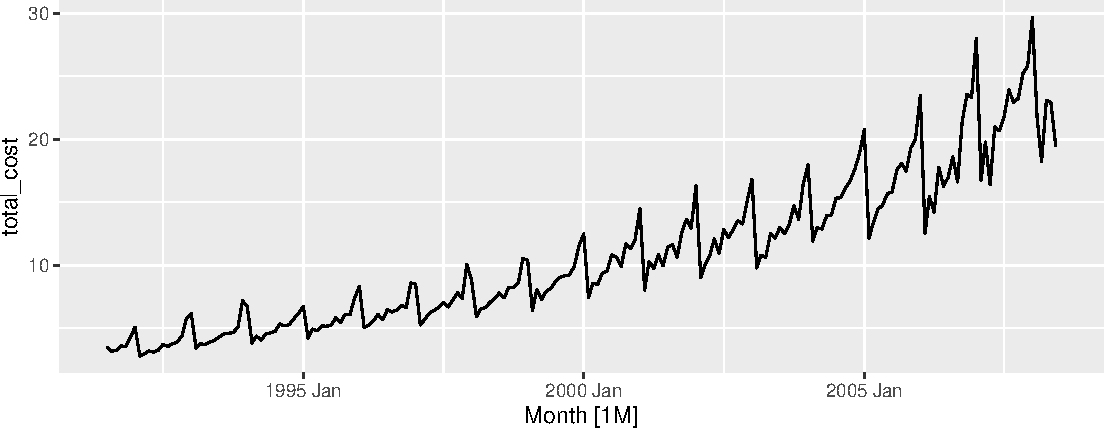
\includegraphics{2-tsgraphics_files/figure-beamer/unnamed-chunk-3-1.pdf}
\end{frame}

\begin{frame}[fragile]{Ansett airlines}
\protect\hypertarget{ansett-airlines}{}
\fontsize{10}{10}\sf

\begin{Shaded}
\begin{Highlighting}[]
\NormalTok{ansett }\SpecialCharTok{\%\textgreater{}\%}
  \FunctionTok{autoplot}\NormalTok{(Passengers)}
\end{Highlighting}
\end{Shaded}

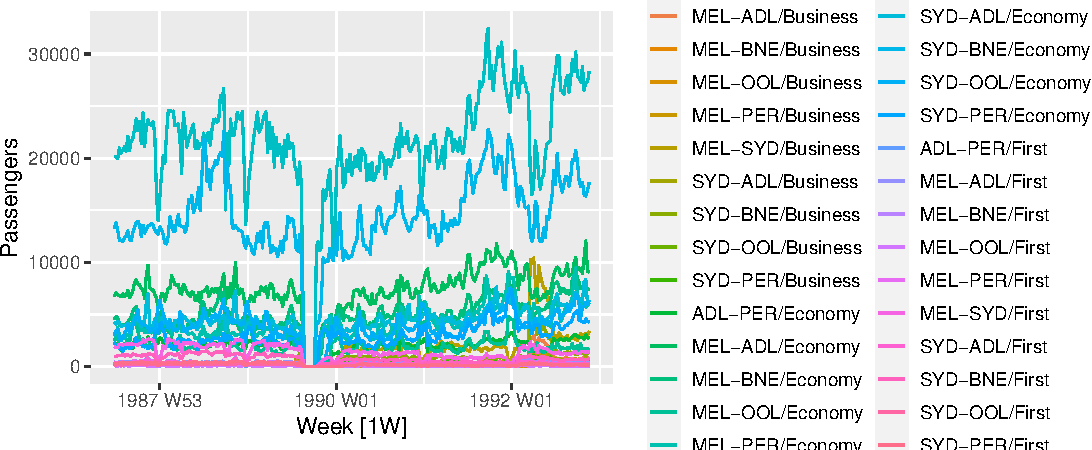
\includegraphics{2-tsgraphics_files/figure-beamer/unnamed-chunk-4-1.pdf}
\end{frame}

\begin{frame}[fragile]{Ansett airlines}
\protect\hypertarget{ansett-airlines-1}{}
\fontsize{10}{10}\sf

\begin{Shaded}
\begin{Highlighting}[]
\NormalTok{ansett }\SpecialCharTok{\%\textgreater{}\%}
  \FunctionTok{filter}\NormalTok{(Class }\SpecialCharTok{==} \StringTok{"Economy"}\NormalTok{) }\SpecialCharTok{\%\textgreater{}\%}
  \FunctionTok{autoplot}\NormalTok{(Passengers)}
\end{Highlighting}
\end{Shaded}

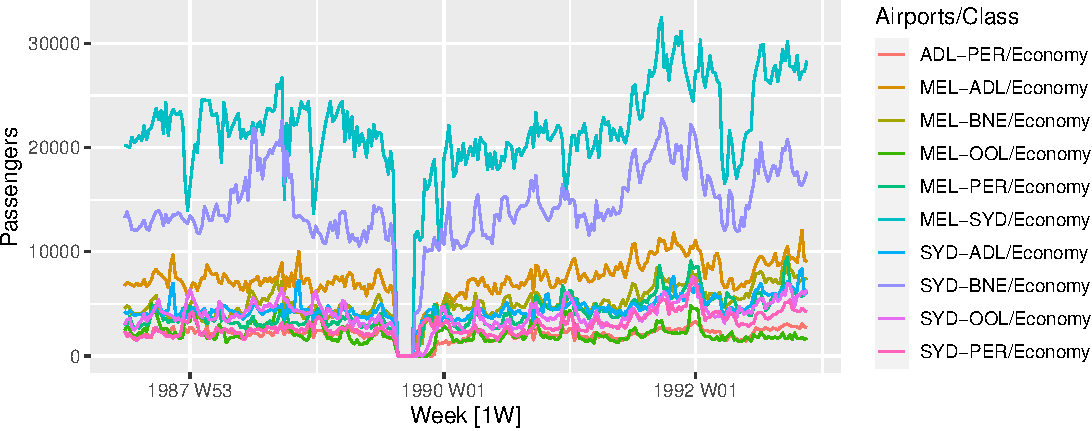
\includegraphics{2-tsgraphics_files/figure-beamer/unnamed-chunk-5-1.pdf}
\end{frame}

\begin{frame}[fragile]{Ansett airlines}
\protect\hypertarget{ansett-airlines-2}{}
\fontsize{10}{10}\sf

\begin{Shaded}
\begin{Highlighting}[]
\NormalTok{ansett }\SpecialCharTok{\%\textgreater{}\%}
  \FunctionTok{filter}\NormalTok{(Airports }\SpecialCharTok{==} \StringTok{"MEL{-}SYD"}\NormalTok{) }\SpecialCharTok{\%\textgreater{}\%}
  \FunctionTok{autoplot}\NormalTok{(Passengers)}
\end{Highlighting}
\end{Shaded}

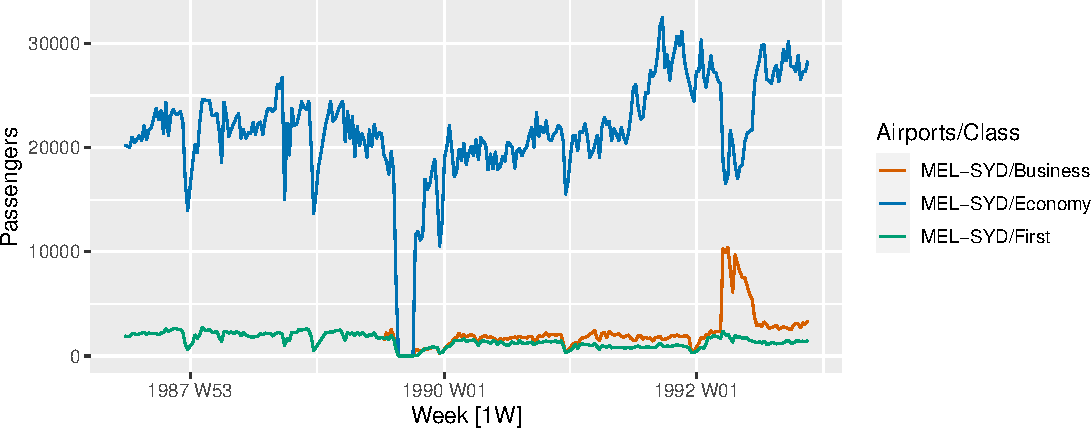
\includegraphics{2-tsgraphics_files/figure-beamer/unnamed-chunk-6-1.pdf}
\end{frame}

\begin{frame}{Time series patterns}
\protect\hypertarget{time-series-patterns}{}
\begin{description}
\tightlist
\item[Trend]
pattern exists when there is a long-term increase or decrease in the
data.
\item[Seasonal]
pattern exists when a series is influenced by seasonal factors (e.g.,
the quarter of the year, the month, or day of the week).
\item[Cyclic]
pattern exists when data exhibit rises and falls that are
\emph{not of fixed period} (duration usually of at least 2 years).
\end{description}
\end{frame}

\begin{frame}{Time series components}
\protect\hypertarget{time-series-components}{}
\begin{block}{Differences between seasonal and cyclic patterns:}
\protect\hypertarget{differences-between-seasonal-and-cyclic-patterns}{}
\begin{itemize}
\tightlist
\item
  seasonal pattern constant length; cyclic pattern variable length
\item
  average length of cycle longer than length of seasonal pattern
\item
  magnitude of cycle more variable than magnitude of seasonal pattern
\end{itemize}
\end{block}
\end{frame}

\begin{frame}[fragile]{Time series patterns}
\protect\hypertarget{time-series-patterns-1}{}
\fontsize{9}{9}\sf

\begin{Shaded}
\begin{Highlighting}[]
\NormalTok{aus\_production }\SpecialCharTok{\%\textgreater{}\%}
  \FunctionTok{filter}\NormalTok{(}\FunctionTok{year}\NormalTok{(Quarter) }\SpecialCharTok{\textgreater{}=} \DecValTok{1980}\NormalTok{) }\SpecialCharTok{\%\textgreater{}\%}
  \FunctionTok{autoplot}\NormalTok{(Electricity) }\SpecialCharTok{+}
  \FunctionTok{labs}\NormalTok{(}\AttributeTok{y =} \StringTok{"GWh"}\NormalTok{, }\AttributeTok{title =} \StringTok{"Australian electricity production"}\NormalTok{)}
\end{Highlighting}
\end{Shaded}

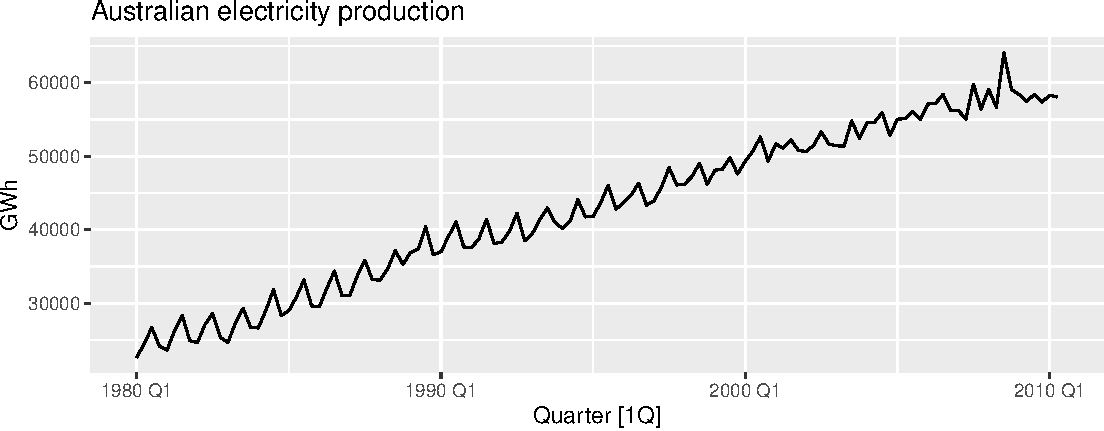
\includegraphics{2-tsgraphics_files/figure-beamer/unnamed-chunk-7-1.pdf}
\end{frame}

\begin{frame}[fragile]{Time series patterns}
\protect\hypertarget{time-series-patterns-2}{}
\fontsize{9}{9}\sf

\begin{Shaded}
\begin{Highlighting}[]
\NormalTok{aus\_production }\SpecialCharTok{\%\textgreater{}\%}
  \FunctionTok{autoplot}\NormalTok{(Bricks) }\SpecialCharTok{+}
  \FunctionTok{labs}\NormalTok{(}\AttributeTok{y =} \StringTok{"million units"}\NormalTok{, }\AttributeTok{title =} \StringTok{"Australian clay brick production"}\NormalTok{)}
\end{Highlighting}
\end{Shaded}

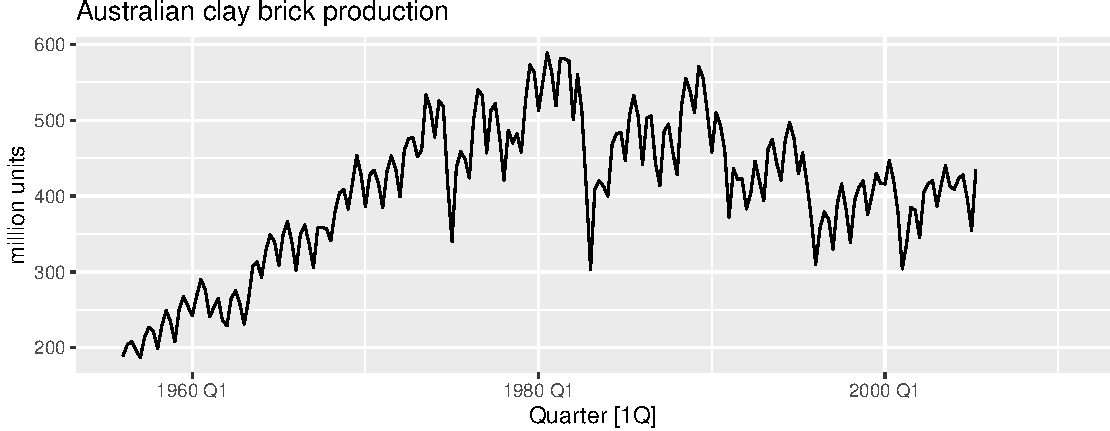
\includegraphics{2-tsgraphics_files/figure-beamer/unnamed-chunk-8-1.pdf}
\end{frame}

\begin{frame}[fragile]{Time series patterns}
\protect\hypertarget{time-series-patterns-3}{}
\fontsize{9}{9}\sf

\begin{Shaded}
\begin{Highlighting}[]
\NormalTok{us\_employment }\SpecialCharTok{\%\textgreater{}\%}
  \FunctionTok{filter}\NormalTok{(Title }\SpecialCharTok{==} \StringTok{"Retail Trade"}\NormalTok{, }\FunctionTok{year}\NormalTok{(Month) }\SpecialCharTok{\textgreater{}=} \DecValTok{1980}\NormalTok{) }\SpecialCharTok{\%\textgreater{}\%}
  \FunctionTok{autoplot}\NormalTok{(Employed }\SpecialCharTok{/} \FloatTok{1e3}\NormalTok{) }\SpecialCharTok{+}
  \FunctionTok{labs}\NormalTok{(}\AttributeTok{y =} \StringTok{"Million people"}\NormalTok{, }\AttributeTok{title =} \StringTok{"Retail employment, USA"}\NormalTok{)}
\end{Highlighting}
\end{Shaded}

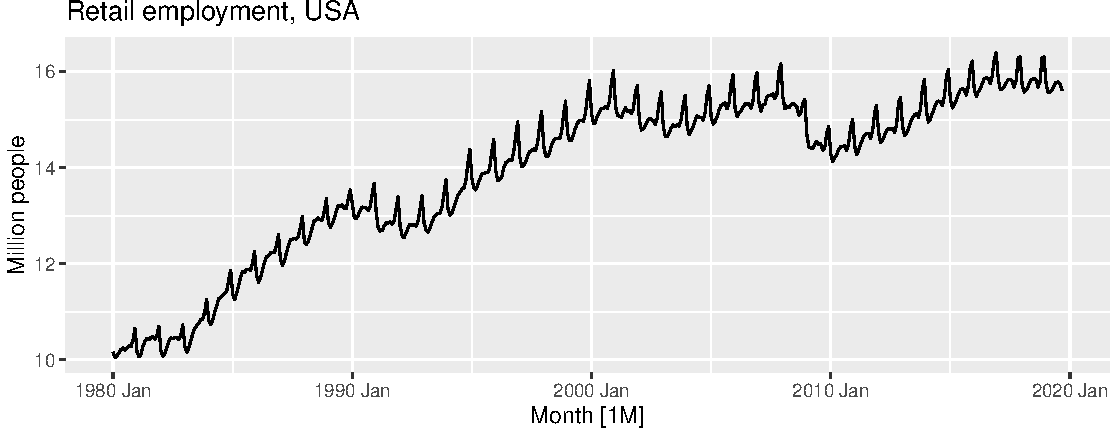
\includegraphics{2-tsgraphics_files/figure-beamer/unnamed-chunk-9-1.pdf}
\end{frame}

\begin{frame}[fragile]{Time series patterns}
\protect\hypertarget{time-series-patterns-4}{}
\fontsize{9}{9}\sf

\begin{Shaded}
\begin{Highlighting}[]
\NormalTok{gafa\_stock }\SpecialCharTok{\%\textgreater{}\%}
  \FunctionTok{filter}\NormalTok{(Symbol }\SpecialCharTok{==} \StringTok{"AMZN"}\NormalTok{, }\FunctionTok{year}\NormalTok{(Date) }\SpecialCharTok{\textgreater{}=} \DecValTok{2018}\NormalTok{) }\SpecialCharTok{\%\textgreater{}\%}
  \FunctionTok{autoplot}\NormalTok{(Close) }\SpecialCharTok{+}
  \FunctionTok{labs}\NormalTok{(}\AttributeTok{y =} \StringTok{"$US"}\NormalTok{, }\AttributeTok{title =} \StringTok{"Amazon closing stock price"}\NormalTok{)}
\end{Highlighting}
\end{Shaded}

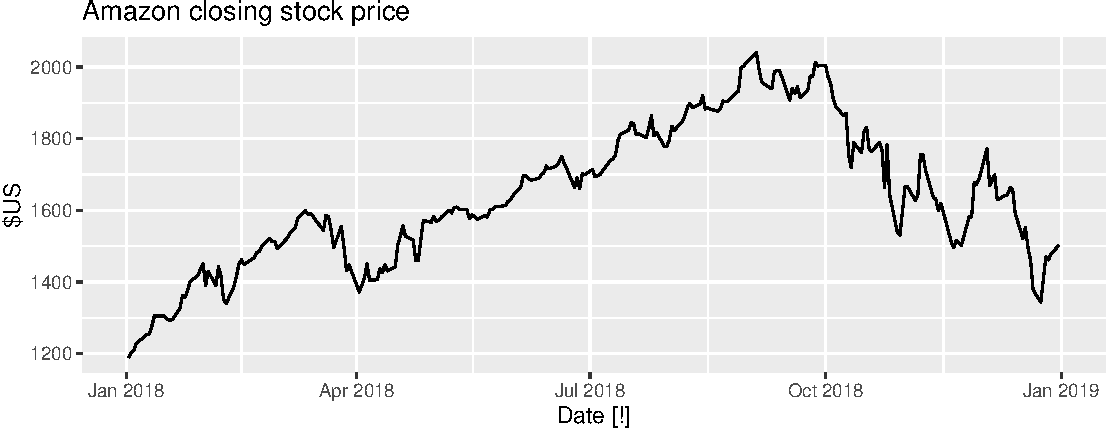
\includegraphics{2-tsgraphics_files/figure-beamer/unnamed-chunk-10-1.pdf}
\end{frame}

\begin{frame}[fragile]{Time series patterns}
\protect\hypertarget{time-series-patterns-5}{}
\fontsize{9}{9}\sf

\begin{Shaded}
\begin{Highlighting}[]
\NormalTok{pelt }\SpecialCharTok{\%\textgreater{}\%}
  \FunctionTok{autoplot}\NormalTok{(Lynx) }\SpecialCharTok{+}
  \FunctionTok{labs}\NormalTok{(}\AttributeTok{y=}\StringTok{"Number trapped"}\NormalTok{, }\AttributeTok{title =} \StringTok{"Annual Canadian Lynx Trappings"}\NormalTok{)}
\end{Highlighting}
\end{Shaded}

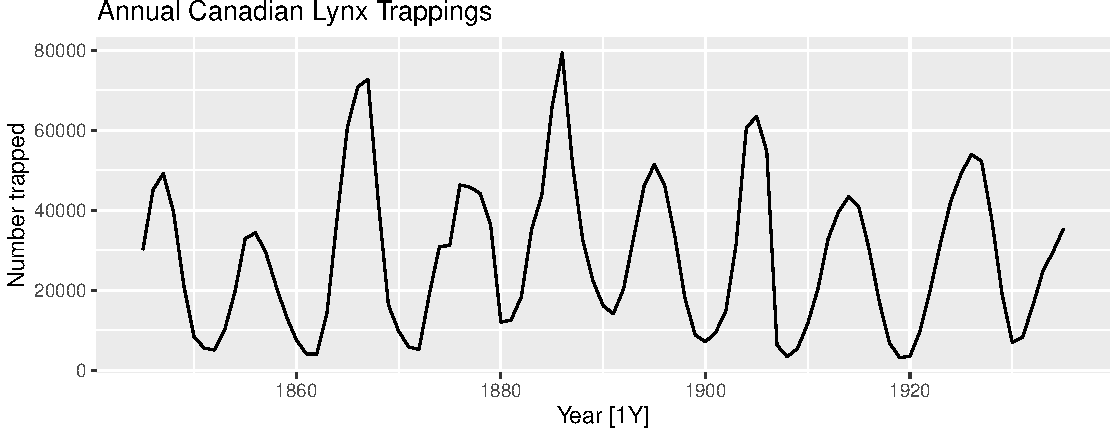
\includegraphics{2-tsgraphics_files/figure-beamer/unnamed-chunk-11-1.pdf}
\end{frame}

\begin{frame}{Seasonal or cyclic?}
\protect\hypertarget{seasonal-or-cyclic}{}
\alert{Differences between seasonal and cyclic patterns:}

\begin{itemize}
\tightlist
\item
  seasonal pattern constant length; cyclic pattern variable length
\item
  average length of cycle longer than length of seasonal pattern
\item
  magnitude of cycle more variable than magnitude of seasonal pattern
\end{itemize}

\pause

\begin{alertblock}{}
The timing of peaks and troughs is predictable with seasonal data, but unpredictable in the long term with cyclic data.
\end{alertblock}
\end{frame}

\hypertarget{seasonal-and-subseries-plots}{%
\section{Seasonal and subseries
plots}\label{seasonal-and-subseries-plots}}

\begin{frame}[fragile]{Seasonal plots}
\protect\hypertarget{seasonal-plots}{}
\fontsize{10}{10}\sf

\begin{Shaded}
\begin{Highlighting}[]
\NormalTok{a10 }\SpecialCharTok{\%\textgreater{}\%} \FunctionTok{gg\_season}\NormalTok{(total\_cost, }\AttributeTok{labels =} \StringTok{"both"}\NormalTok{) }\SpecialCharTok{+}
  \FunctionTok{labs}\NormalTok{(}\AttributeTok{y =} \StringTok{"$ million"}\NormalTok{, }\AttributeTok{title =} \StringTok{"Seasonal plot: antidiabetic drug sales"}\NormalTok{)}
\end{Highlighting}
\end{Shaded}

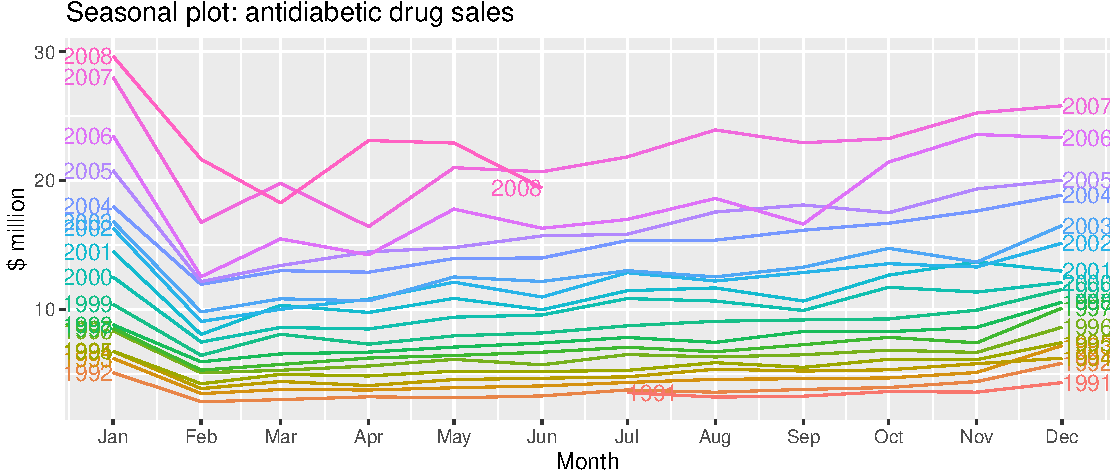
\includegraphics{2-tsgraphics_files/figure-beamer/unnamed-chunk-12-1.pdf}
\end{frame}

\begin{frame}[fragile]{Seasonal plots}
\protect\hypertarget{seasonal-plots-1}{}
\begin{itemize}
\tightlist
\item
  Data plotted against the individual ``seasons'' in which the data were
  observed. (In this case a ``season'' is a month.)
\item
  Something like a time plot except that the data from each season are
  overlapped.
\item
  Enables the underlying seasonal pattern to be seen more clearly, and
  also allows any substantial departures from the seasonal pattern to be
  easily identified.
\item
  In R: \texttt{gg\_season()}
\end{itemize}
\end{frame}

\begin{frame}[fragile]{Seasonal subseries plots}
\protect\hypertarget{seasonal-subseries-plots}{}
\fontsize{10}{10}\sf

\begin{Shaded}
\begin{Highlighting}[]
\NormalTok{a10 }\SpecialCharTok{\%\textgreater{}\%}
  \FunctionTok{gg\_subseries}\NormalTok{(total\_cost) }\SpecialCharTok{+}
  \FunctionTok{labs}\NormalTok{(}\AttributeTok{y =} \StringTok{"$ million"}\NormalTok{, }\AttributeTok{title =} \StringTok{"Subseries plot: antidiabetic drug sales"}\NormalTok{)}
\end{Highlighting}
\end{Shaded}

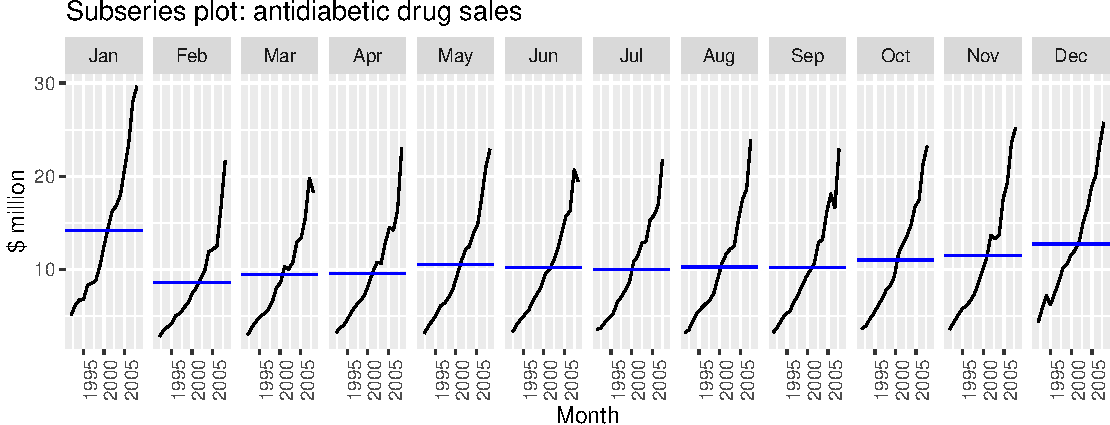
\includegraphics{2-tsgraphics_files/figure-beamer/unnamed-chunk-13-1.pdf}
\end{frame}

\begin{frame}[fragile]{Seasonal subseries plots}
\protect\hypertarget{seasonal-subseries-plots-1}{}
\begin{itemize}
\tightlist
\item
  Data for each season collected together in time plot as separate time
  series.
\item
  Enables the underlying seasonal pattern to be seen clearly, and
  changes in seasonality over time to be visualized.
\item
  In R: \texttt{gg\_subseries()}
\end{itemize}
\end{frame}

\begin{frame}[fragile]{Quarterly Australian Beer Production}
\protect\hypertarget{quarterly-australian-beer-production}{}
\fontsize{9}{9}\sf

\begin{Shaded}
\begin{Highlighting}[]
\NormalTok{beer }\OtherTok{\textless{}{-}}\NormalTok{ aus\_production }\SpecialCharTok{\%\textgreater{}\%}
  \FunctionTok{select}\NormalTok{(Quarter, Beer) }\SpecialCharTok{\%\textgreater{}\%}
  \FunctionTok{filter}\NormalTok{(}\FunctionTok{year}\NormalTok{(Quarter) }\SpecialCharTok{\textgreater{}=} \DecValTok{1992}\NormalTok{)}
\NormalTok{beer }\SpecialCharTok{\%\textgreater{}\%} \FunctionTok{autoplot}\NormalTok{(Beer)}
\end{Highlighting}
\end{Shaded}

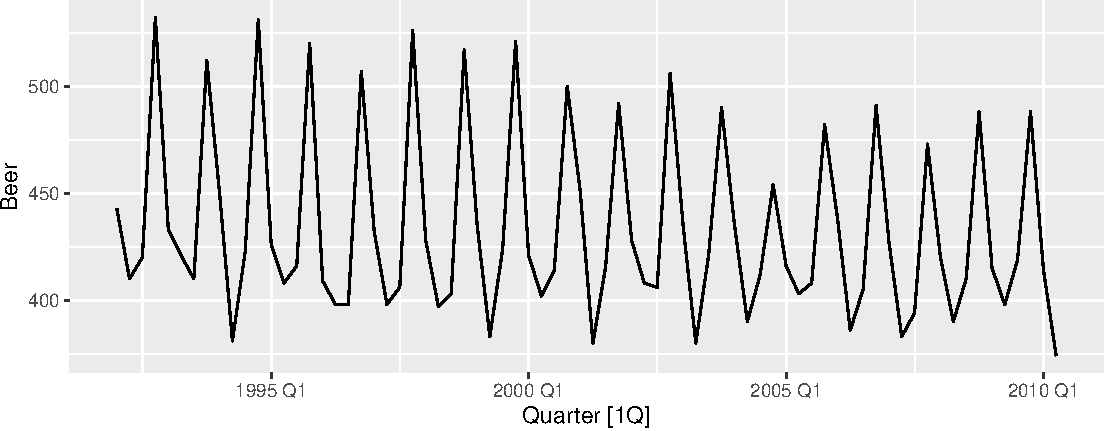
\includegraphics{2-tsgraphics_files/figure-beamer/unnamed-chunk-14-1.pdf}
\end{frame}

\begin{frame}[fragile]{Quarterly Australian Beer Production}
\protect\hypertarget{quarterly-australian-beer-production-1}{}
\fontsize{9}{9}\sf

\begin{Shaded}
\begin{Highlighting}[]
\NormalTok{beer }\SpecialCharTok{\%\textgreater{}\%} \FunctionTok{gg\_season}\NormalTok{(Beer, }\AttributeTok{labels=}\StringTok{"right"}\NormalTok{)}
\end{Highlighting}
\end{Shaded}

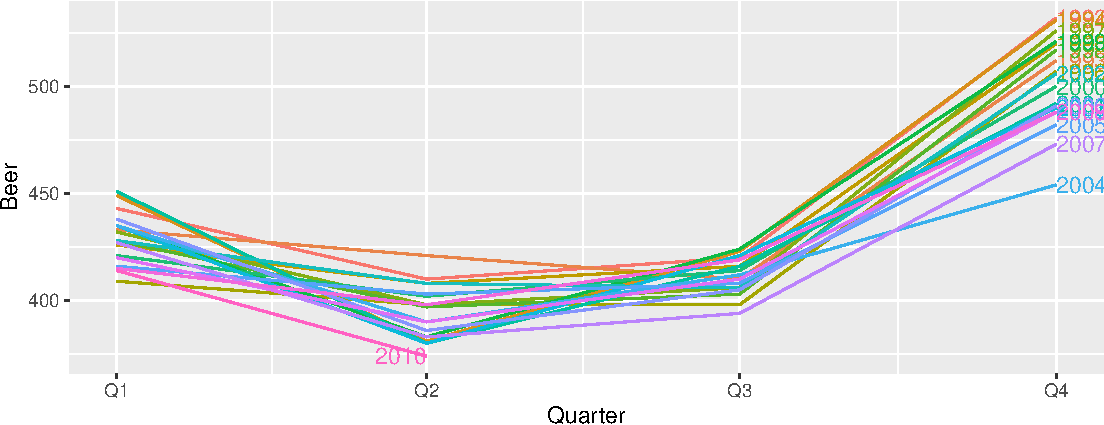
\includegraphics{2-tsgraphics_files/figure-beamer/unnamed-chunk-15-1.pdf}
\end{frame}

\begin{frame}[fragile]{Quarterly Australian Beer Production}
\protect\hypertarget{quarterly-australian-beer-production-2}{}
\fontsize{9}{9}\sf

\begin{Shaded}
\begin{Highlighting}[]
\NormalTok{beer }\SpecialCharTok{\%\textgreater{}\%} \FunctionTok{gg\_subseries}\NormalTok{(Beer)}
\end{Highlighting}
\end{Shaded}

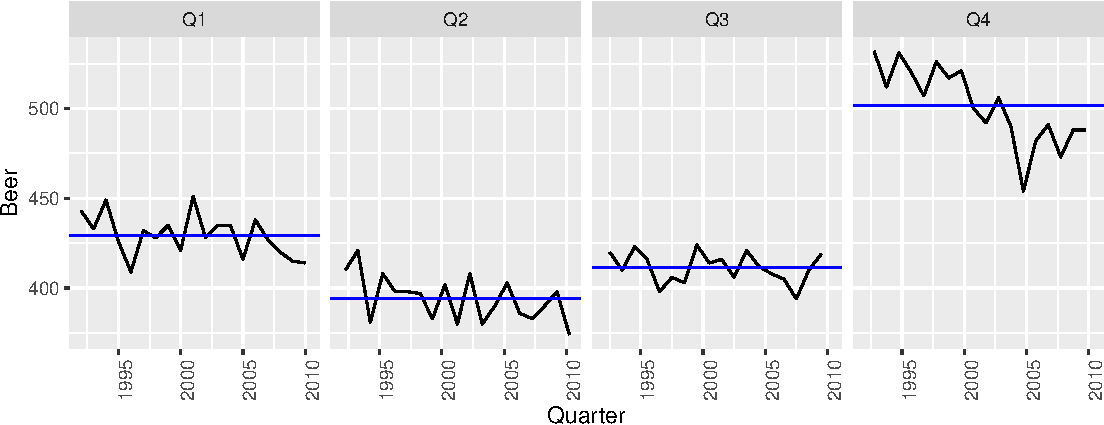
\includegraphics{2-tsgraphics_files/figure-beamer/unnamed-chunk-16-1.pdf}
\end{frame}

\begin{frame}[fragile]{Multiple seasonal periods}
\protect\hypertarget{multiple-seasonal-periods}{}
\fontsize{9}{9}\sf

\begin{Shaded}
\begin{Highlighting}[]
\NormalTok{vic\_elec}
\end{Highlighting}
\end{Shaded}

\begin{verbatim}
## # A tsibble: 52,608 x 5 [30m] <Australia/Melbourne>
##    Time                Demand Temperature Date       Holiday
##    <dttm>               <dbl>       <dbl> <date>     <lgl>  
##  1 2012-01-01 00:00:00  4383.        21.4 2012-01-01 TRUE   
##  2 2012-01-01 00:30:00  4263.        21.0 2012-01-01 TRUE   
##  3 2012-01-01 01:00:00  4049.        20.7 2012-01-01 TRUE   
##  4 2012-01-01 01:30:00  3878.        20.6 2012-01-01 TRUE   
##  5 2012-01-01 02:00:00  4036.        20.4 2012-01-01 TRUE   
##  6 2012-01-01 02:30:00  3866.        20.2 2012-01-01 TRUE   
##  7 2012-01-01 03:00:00  3694.        20.1 2012-01-01 TRUE   
##  8 2012-01-01 03:30:00  3562.        19.6 2012-01-01 TRUE   
##  9 2012-01-01 04:00:00  3433.        19.1 2012-01-01 TRUE   
## 10 2012-01-01 04:30:00  3359.        19.0 2012-01-01 TRUE   
## # ... with 52,598 more rows
## # i Use `print(n = ...)` to see more rows
\end{verbatim}
\end{frame}

\begin{frame}[fragile]{Multiple seasonal periods}
\protect\hypertarget{multiple-seasonal-periods-1}{}
\fontsize{9}{9}\sf

\begin{Shaded}
\begin{Highlighting}[]
\NormalTok{vic\_elec }\SpecialCharTok{\%\textgreater{}\%} \FunctionTok{gg\_season}\NormalTok{(Demand)}
\end{Highlighting}
\end{Shaded}

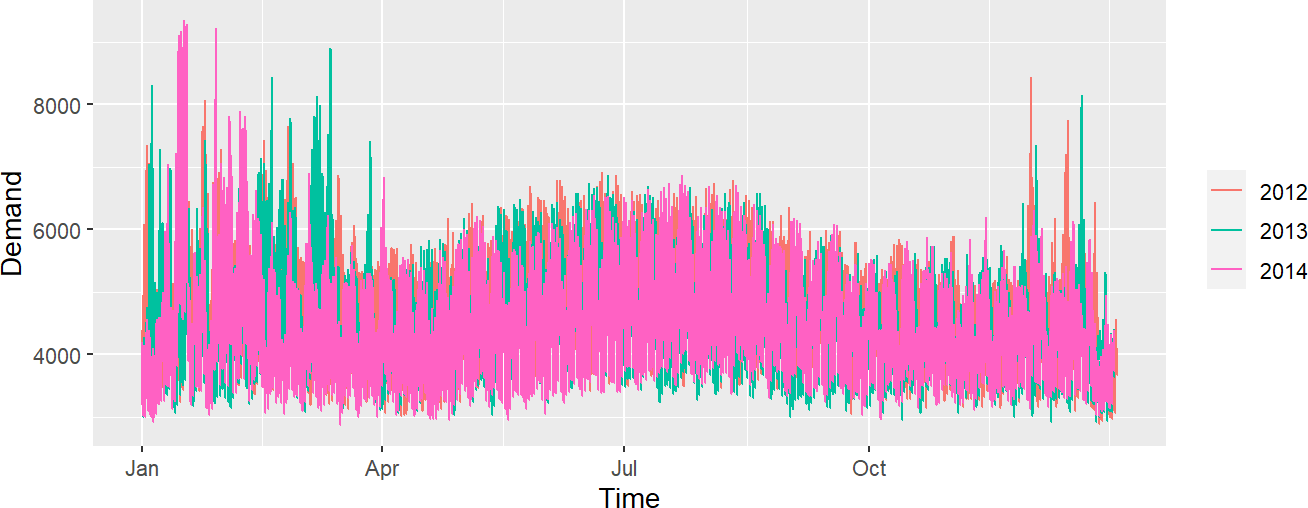
\includegraphics{2-tsgraphics_files/figure-beamer/unnamed-chunk-18-1.png}
\end{frame}

\begin{frame}[fragile]{Multiple seasonal periods}
\protect\hypertarget{multiple-seasonal-periods-2}{}
\fontsize{9}{9}\sf

\begin{Shaded}
\begin{Highlighting}[]
\NormalTok{vic\_elec }\SpecialCharTok{\%\textgreater{}\%} \FunctionTok{gg\_season}\NormalTok{(Demand, }\AttributeTok{period =} \StringTok{"week"}\NormalTok{)}
\end{Highlighting}
\end{Shaded}

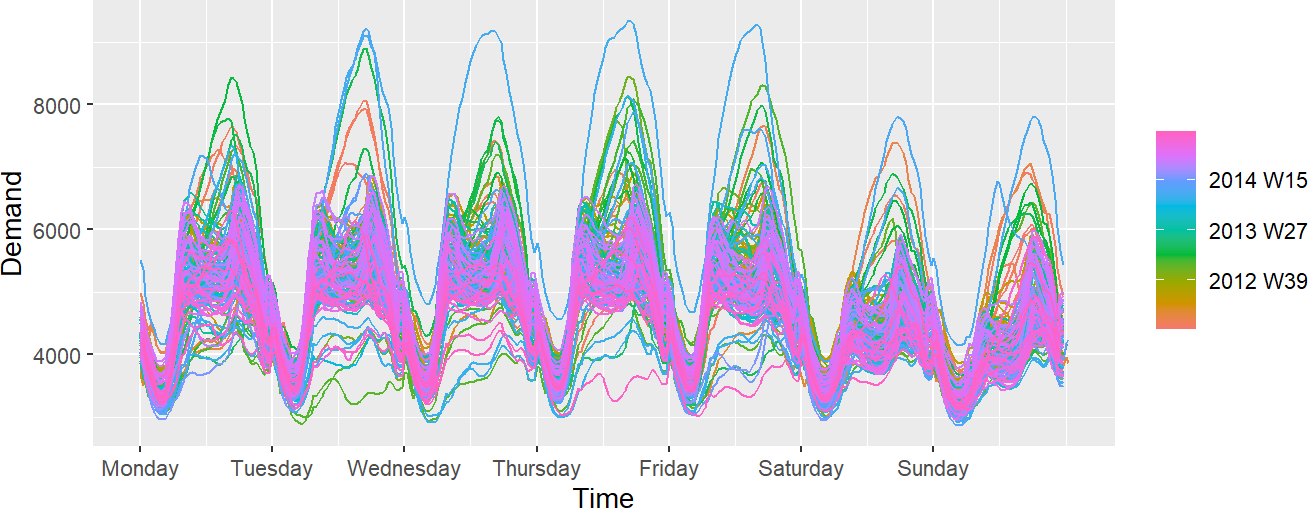
\includegraphics{2-tsgraphics_files/figure-beamer/unnamed-chunk-19-1.png}
\end{frame}

\begin{frame}[fragile]{Multiple seasonal periods}
\protect\hypertarget{multiple-seasonal-periods-3}{}
\fontsize{9}{9}\sf

\begin{Shaded}
\begin{Highlighting}[]
\NormalTok{vic\_elec }\SpecialCharTok{\%\textgreater{}\%} \FunctionTok{gg\_season}\NormalTok{(Demand, }\AttributeTok{period =} \StringTok{"day"}\NormalTok{)}
\end{Highlighting}
\end{Shaded}

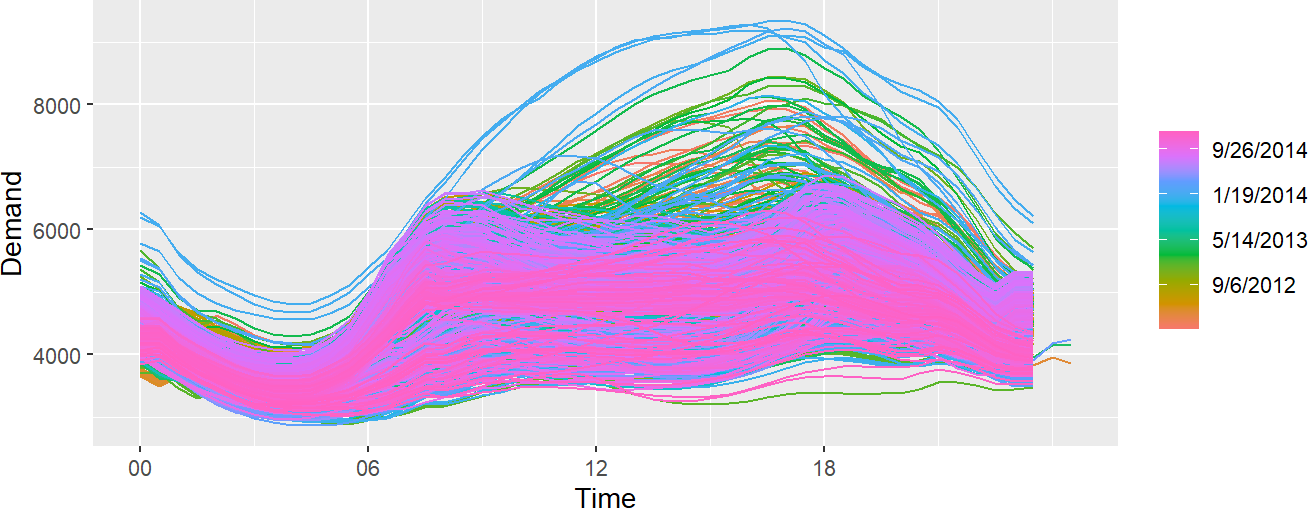
\includegraphics{2-tsgraphics_files/figure-beamer/unnamed-chunk-20-1.png}
\end{frame}

\begin{frame}[fragile]{Australian holidays}
\protect\hypertarget{australian-holidays}{}
\fontsize{9}{10}\sf

\begin{Shaded}
\begin{Highlighting}[]
\NormalTok{holidays }\OtherTok{\textless{}{-}}\NormalTok{ tourism }\SpecialCharTok{\%\textgreater{}\%}
  \FunctionTok{filter}\NormalTok{(Purpose }\SpecialCharTok{==} \StringTok{"Holiday"}\NormalTok{) }\SpecialCharTok{\%\textgreater{}\%}
  \FunctionTok{group\_by}\NormalTok{(State) }\SpecialCharTok{\%\textgreater{}\%}
  \FunctionTok{summarise}\NormalTok{(}\AttributeTok{Trips =} \FunctionTok{sum}\NormalTok{(Trips))}
\end{Highlighting}
\end{Shaded}

\begin{verbatim}
## # A tsibble: 640 x 3 [1Q]
## # Key:       State [8]
##    State Quarter Trips
##    <chr>   <qtr> <dbl>
##  1 ACT   1998 Q1  196.
##  2 ACT   1998 Q2  127.
##  3 ACT   1998 Q3  111.
##  4 ACT   1998 Q4  170.
##  5 ACT   1999 Q1  108.
##  6 ACT   1999 Q2  125.
##  7 ACT   1999 Q3  178.
##  8 ACT   1999 Q4  218.
##  9 ACT   2000 Q1  158.
## 10 ACT   2000 Q2  155.
## # ... with 630 more rows
## # i Use `print(n = ...)` to see more rows
\end{verbatim}
\end{frame}

\begin{frame}[fragile]{Australian holidays}
\protect\hypertarget{australian-holidays-1}{}
\fontsize{9}{10}\sf

\begin{Shaded}
\begin{Highlighting}[]
\NormalTok{holidays }\SpecialCharTok{\%\textgreater{}\%} \FunctionTok{autoplot}\NormalTok{(Trips) }\SpecialCharTok{+}
  \FunctionTok{labs}\NormalTok{(}\AttributeTok{y =} \StringTok{"thousands of trips"}\NormalTok{, }\AttributeTok{title =} \StringTok{"Australian domestic holiday nights"}\NormalTok{)}
\end{Highlighting}
\end{Shaded}

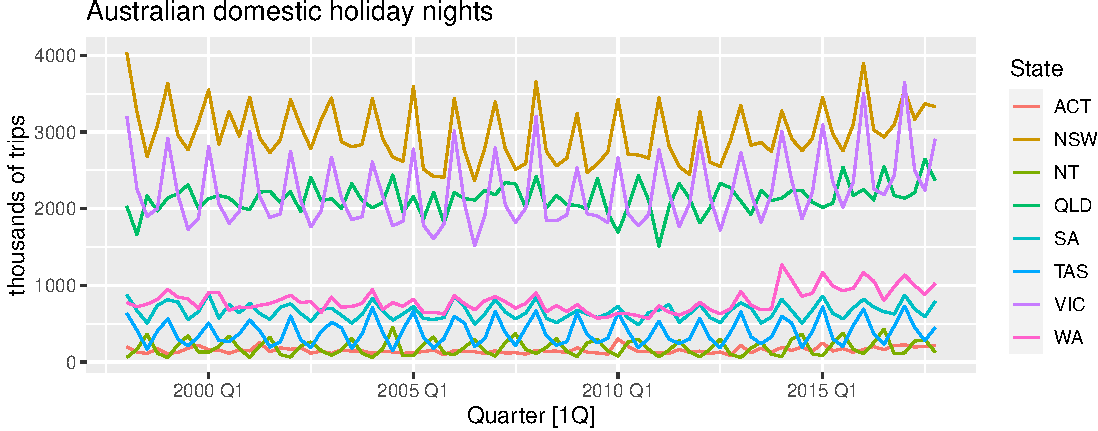
\includegraphics{2-tsgraphics_files/figure-beamer/holidays-plot-1.pdf}
\end{frame}

\begin{frame}[fragile]{Seasonal plots}
\protect\hypertarget{seasonal-plots-2}{}
\fontsize{9}{10}\sf

\begin{Shaded}
\begin{Highlighting}[]
\NormalTok{holidays }\SpecialCharTok{\%\textgreater{}\%} \FunctionTok{gg\_season}\NormalTok{(Trips) }\SpecialCharTok{+}
  \FunctionTok{labs}\NormalTok{(}\AttributeTok{y =} \StringTok{"thousands of trips"}\NormalTok{, }\AttributeTok{title =} \StringTok{"Australian domestic holiday nights"}\NormalTok{)}
\end{Highlighting}
\end{Shaded}

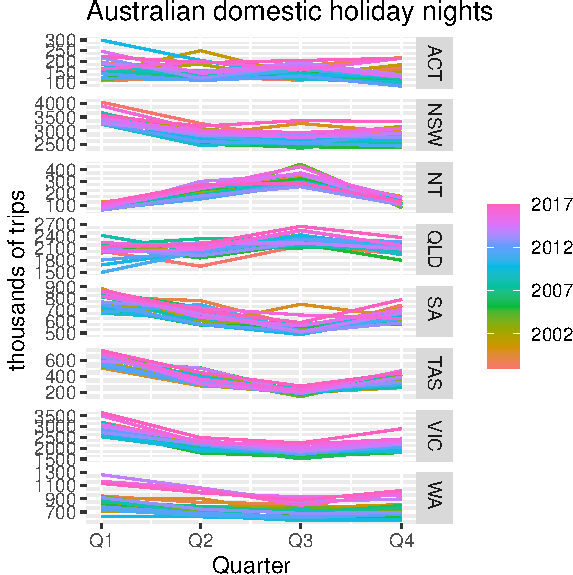
\includegraphics[width=0.45\linewidth]{2-tsgraphics_files/figure-beamer/graphics1-1}
\end{frame}

\begin{frame}[fragile]{Seasonal subseries plots}
\protect\hypertarget{seasonal-subseries-plots-2}{}
\fontsize{9}{10}\sf

\begin{Shaded}
\begin{Highlighting}[]
\NormalTok{holidays }\SpecialCharTok{\%\textgreater{}\%}
  \FunctionTok{gg\_subseries}\NormalTok{(Trips) }\SpecialCharTok{+}
  \FunctionTok{labs}\NormalTok{(}\AttributeTok{y =} \StringTok{"thousands of trips"}\NormalTok{, }\AttributeTok{title =} \StringTok{"Australian domestic holiday nights"}\NormalTok{)}
\end{Highlighting}
\end{Shaded}

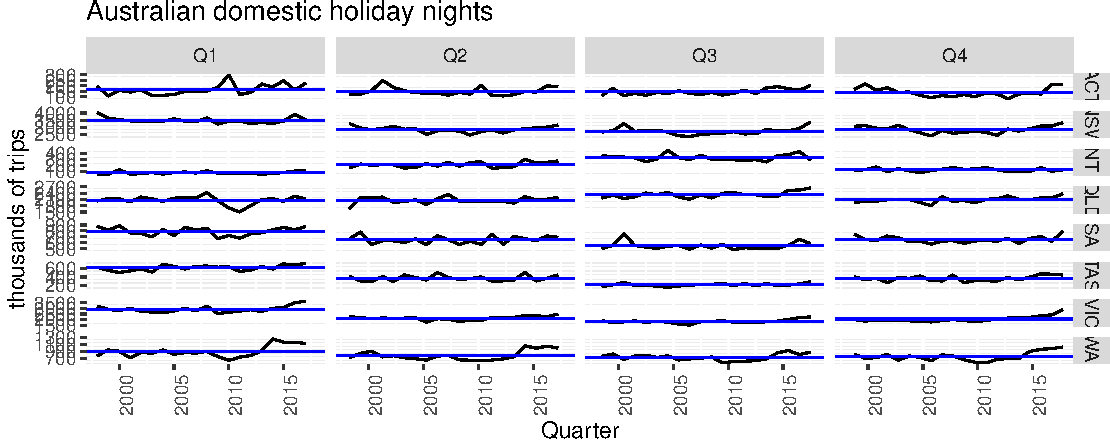
\includegraphics{2-tsgraphics_files/figure-beamer/graphics2-1.pdf}
\end{frame}

\hypertarget{lag-plots-and-autocorrelation}{%
\section{Lag plots and
autocorrelation}\label{lag-plots-and-autocorrelation}}

\begin{frame}[fragile]{Example: Beer production}
\protect\hypertarget{example-beer-production}{}
\fontsize{10}{10}\sf

\begin{Shaded}
\begin{Highlighting}[]
\NormalTok{new\_production }\OtherTok{\textless{}{-}}\NormalTok{ aus\_production }\SpecialCharTok{\%\textgreater{}\%}
  \FunctionTok{filter}\NormalTok{(}\FunctionTok{year}\NormalTok{(Quarter) }\SpecialCharTok{\textgreater{}=} \DecValTok{1992}\NormalTok{)}
\NormalTok{new\_production}
\end{Highlighting}
\end{Shaded}

\begin{verbatim}
## # A tsibble: 74 x 7 [1Q]
##    Quarter  Beer Tobacco Bricks Cement Electricity   Gas
##      <qtr> <dbl>   <dbl>  <dbl>  <dbl>       <dbl> <dbl>
##  1 1992 Q1   443    5777    383   1289       38332   117
##  2 1992 Q2   410    5853    404   1501       39774   151
##  3 1992 Q3   420    6416    446   1539       42246   175
##  4 1992 Q4   532    5825    420   1568       38498   129
##  5 1993 Q1   433    5724    394   1450       39460   116
##  6 1993 Q2   421    6036    462   1668       41356   149
##  7 1993 Q3   410    6570    475   1648       42949   163
##  8 1993 Q4   512    5675    443   1863       40974   138
##  9 1994 Q1   449    5311    421   1468       40162   127
## 10 1994 Q2   381    5717    475   1755       41199   159
## # ... with 64 more rows
## # i Use `print(n = ...)` to see more rows
\end{verbatim}
\end{frame}

\begin{frame}[fragile]{Example: Beer production}
\protect\hypertarget{example-beer-production-1}{}
\fontsize{10}{10}\sf

\begin{Shaded}
\begin{Highlighting}[]
\NormalTok{new\_production }\SpecialCharTok{\%\textgreater{}\%} \FunctionTok{gg\_lag}\NormalTok{(Beer)}
\end{Highlighting}
\end{Shaded}

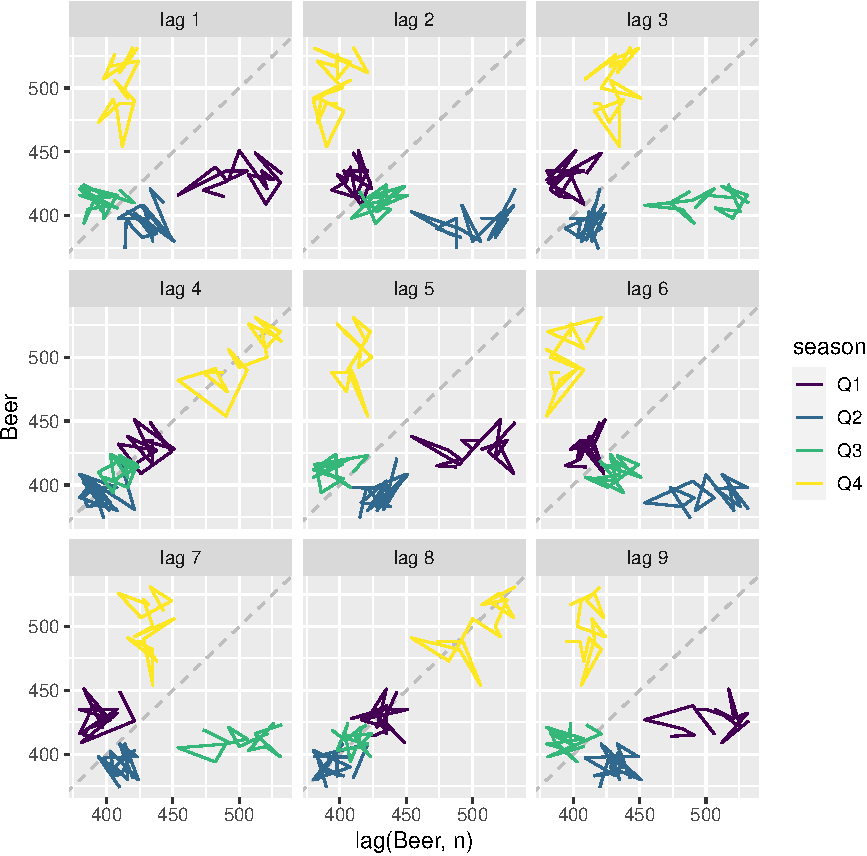
\includegraphics[width=6.5cm]{2-tsgraphics_files/figure-beamer/unnamed-chunk-23-1}
\end{frame}

\begin{frame}[fragile]{Example: Beer production}
\protect\hypertarget{example-beer-production-2}{}
\fontsize{10}{10}\sf

\begin{Shaded}
\begin{Highlighting}[]
\NormalTok{new\_production }\SpecialCharTok{\%\textgreater{}\%} \FunctionTok{gg\_lag}\NormalTok{(Beer, }\AttributeTok{geom=}\StringTok{\textquotesingle{}point\textquotesingle{}}\NormalTok{)}
\end{Highlighting}
\end{Shaded}

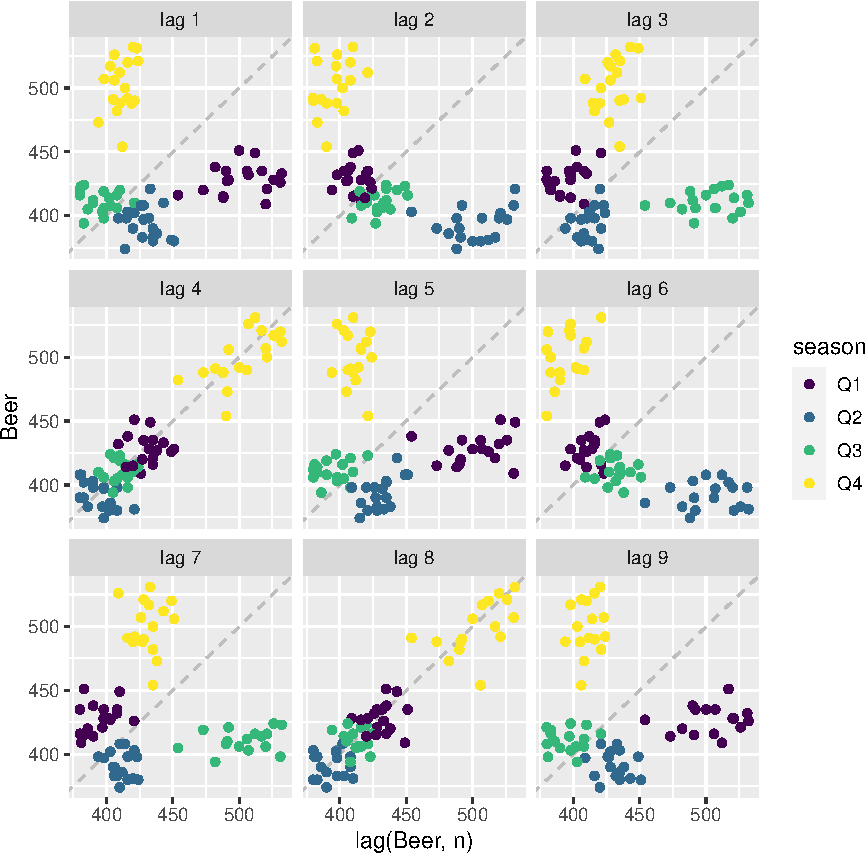
\includegraphics[width=6.5cm]{2-tsgraphics_files/figure-beamer/unnamed-chunk-24-1}
\end{frame}

\begin{frame}{Lagged scatterplots}
\protect\hypertarget{lagged-scatterplots}{}
\begin{itemize}
\tightlist
\item
  Each graph shows \(y_t\) plotted against \(y_{t-k}\) for different
  values of \(k\).
\item
  The autocorrelations are the correlations associated with these
  scatterplots.
\item
  ACF (autocorrelation function):

  \begin{itemize}
  \tightlist
  \item
    \(r_1=\text{Correlation}(y_{t}, y_{t-1})\)
  \item
    \(r_2=\text{Correlation}(y_{t}, y_{t-2})\)
  \item
    \(r_3=\text{Correlation}(y_{t}, y_{t-3})\)
  \item
    etc.
  \end{itemize}
\end{itemize}
\end{frame}

\begin{frame}{Autocorrelation}
\protect\hypertarget{autocorrelation}{}
\textbf{Covariance} and \textbf{correlation}: measure extent of
\textbf{linear relationship} between two variables (\(y\) and
\(X\)).\pause

\textbf{Autocovariance} and \textbf{autocorrelation}: measure linear
relationship between \textbf{lagged values} of a time series
\(y\).\pause

We measure the relationship between:

\begin{itemize}
\tightlist
\item
  \(y_{t}\) and \(y_{t-1}\)
\item
  \(y_{t}\) and \(y_{t-2}\)
\item
  \(y_{t}\) and \(y_{t-3}\)
\item
  etc.
\end{itemize}
\end{frame}

\begin{frame}{Autocorrelation}
\protect\hypertarget{autocorrelation-1}{}
We denote the sample autocovariance at lag \(k\) by \(c_k\) and the
sample autocorrelation at lag \(k\) by \(r_k\). Then define

\begin{block}{}
\begin{align*}
c_k &= \frac{1}{T}\sum_{t=k+1}^T (y_t-\bar{y})(y_{t-k}-\bar{y}) \\[0.cm]
\text{and}\qquad
r_{k} &= c_k/c_0
\end{align*}
\end{block}\pause\small

\begin{itemize}
\tightlist
\item
  \(r_1\) indicates how successive values of \(y\) relate to each other
\item
  \(r_2\) indicates how \(y\) values two periods apart relate to each
  other
\item
  \(r_k\) is \textit{almost} the same as the sample correlation between
  \(y_t\) and \(y_{t-k}\).
\end{itemize}
\end{frame}

\begin{frame}[fragile]{Autocorrelation}
\protect\hypertarget{autocorrelation-2}{}
Results for first 9 lags for beer data:

\fontsize{11}{13}\sf

\begin{Shaded}
\begin{Highlighting}[]
\NormalTok{new\_production }\SpecialCharTok{\%\textgreater{}\%} \FunctionTok{ACF}\NormalTok{(Beer, }\AttributeTok{lag\_max =} \DecValTok{9}\NormalTok{)}
\end{Highlighting}
\end{Shaded}

\begin{verbatim}
## # A tsibble: 9 x 2 [1Q]
##     lag     acf
##   <lag>   <dbl>
## 1    1Q -0.102 
## 2    2Q -0.657 
## 3    3Q -0.0603
## 4    4Q  0.869 
## 5    5Q -0.0892
## 6    6Q -0.635 
## 7    7Q -0.0542
## 8    8Q  0.832 
## 9    9Q -0.108
\end{verbatim}
\end{frame}

\begin{frame}[fragile]{Autocorrelation}
\protect\hypertarget{autocorrelation-3}{}
Results for first 9 lags for beer data:

\fontsize{11}{13}\sf

\begin{Shaded}
\begin{Highlighting}[]
\NormalTok{new\_production }\SpecialCharTok{\%\textgreater{}\%} \FunctionTok{ACF}\NormalTok{(Beer, }\AttributeTok{lag\_max =} \DecValTok{9}\NormalTok{) }\SpecialCharTok{\%\textgreater{}\%} \FunctionTok{autoplot}\NormalTok{()}
\end{Highlighting}
\end{Shaded}

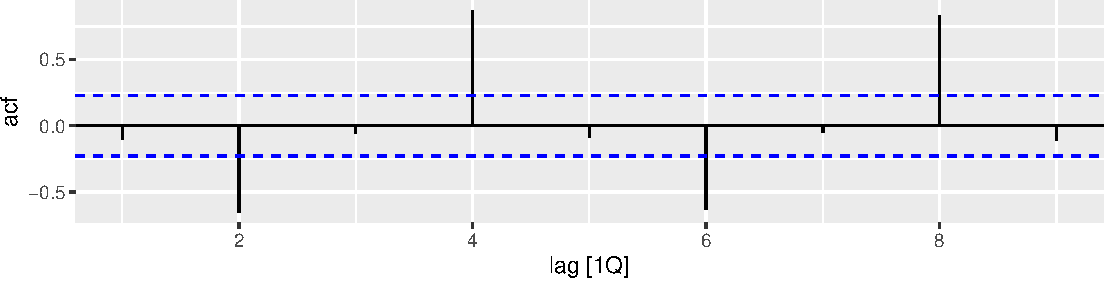
\includegraphics{2-tsgraphics_files/figure-beamer/beeracf-1.pdf}

\begin{itemize}
\tightlist
\item
  Together, the autocorrelations at lags 1, 2, \dots, make up the
  \emph{autocorrelation} or ACF.
\item
  The plot is known as a \textbf{correlogram}
\end{itemize}

\vspace*{10cm}
\end{frame}

\begin{frame}[fragile]{Autocorrelation}
\protect\hypertarget{autocorrelation-4}{}
\fontsize{11}{13}\sf

\begin{Shaded}
\begin{Highlighting}[]
\NormalTok{new\_production }\SpecialCharTok{\%\textgreater{}\%} \FunctionTok{ACF}\NormalTok{(Beer) }\SpecialCharTok{\%\textgreater{}\%} \FunctionTok{autoplot}\NormalTok{()}
\end{Highlighting}
\end{Shaded}

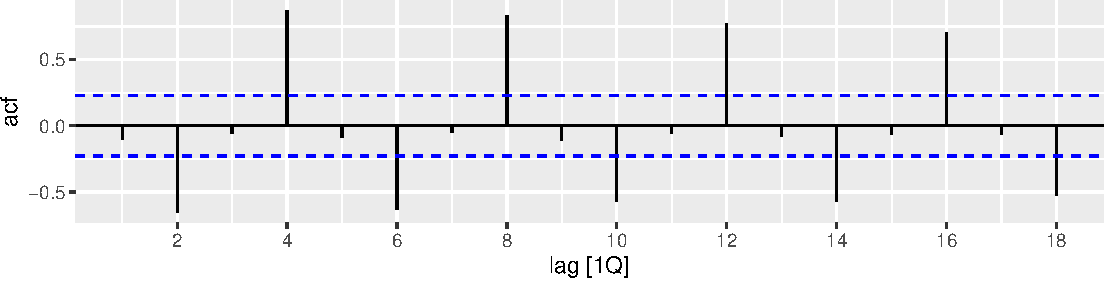
\includegraphics{2-tsgraphics_files/figure-beamer/beeracf2-1.pdf}

\begin{itemize}
\tightlist
\item
  \(r_{4}\) higher than for the other lags. This is due to \textbf{the
  seasonal pattern in the data}: the peaks tend to be \textbf{4
  quarters} apart and the troughs tend to be \textbf{2 quarters} apart.
\item
  \(r_2\) is more negative than for the other lags because troughs tend
  to be 2 quarters behind peaks.
\end{itemize}
\end{frame}

\begin{frame}{Trend and seasonality in ACF plots}
\protect\hypertarget{trend-and-seasonality-in-acf-plots}{}
\begin{itemize}
\tightlist
\item
  When data have a trend, the autocorrelations for small lags tend to be
  large and positive.
\item
  When data are seasonal, the autocorrelations will be larger at the
  seasonal lags (i.e., at multiples of the seasonal frequency)
\item
  When data are trended and seasonal, you see a combination of these
  effects.
\end{itemize}
\end{frame}

\begin{frame}{Autocorrelation functions}
\protect\hypertarget{autocorrelation-functions}{}
\only<1>{\centering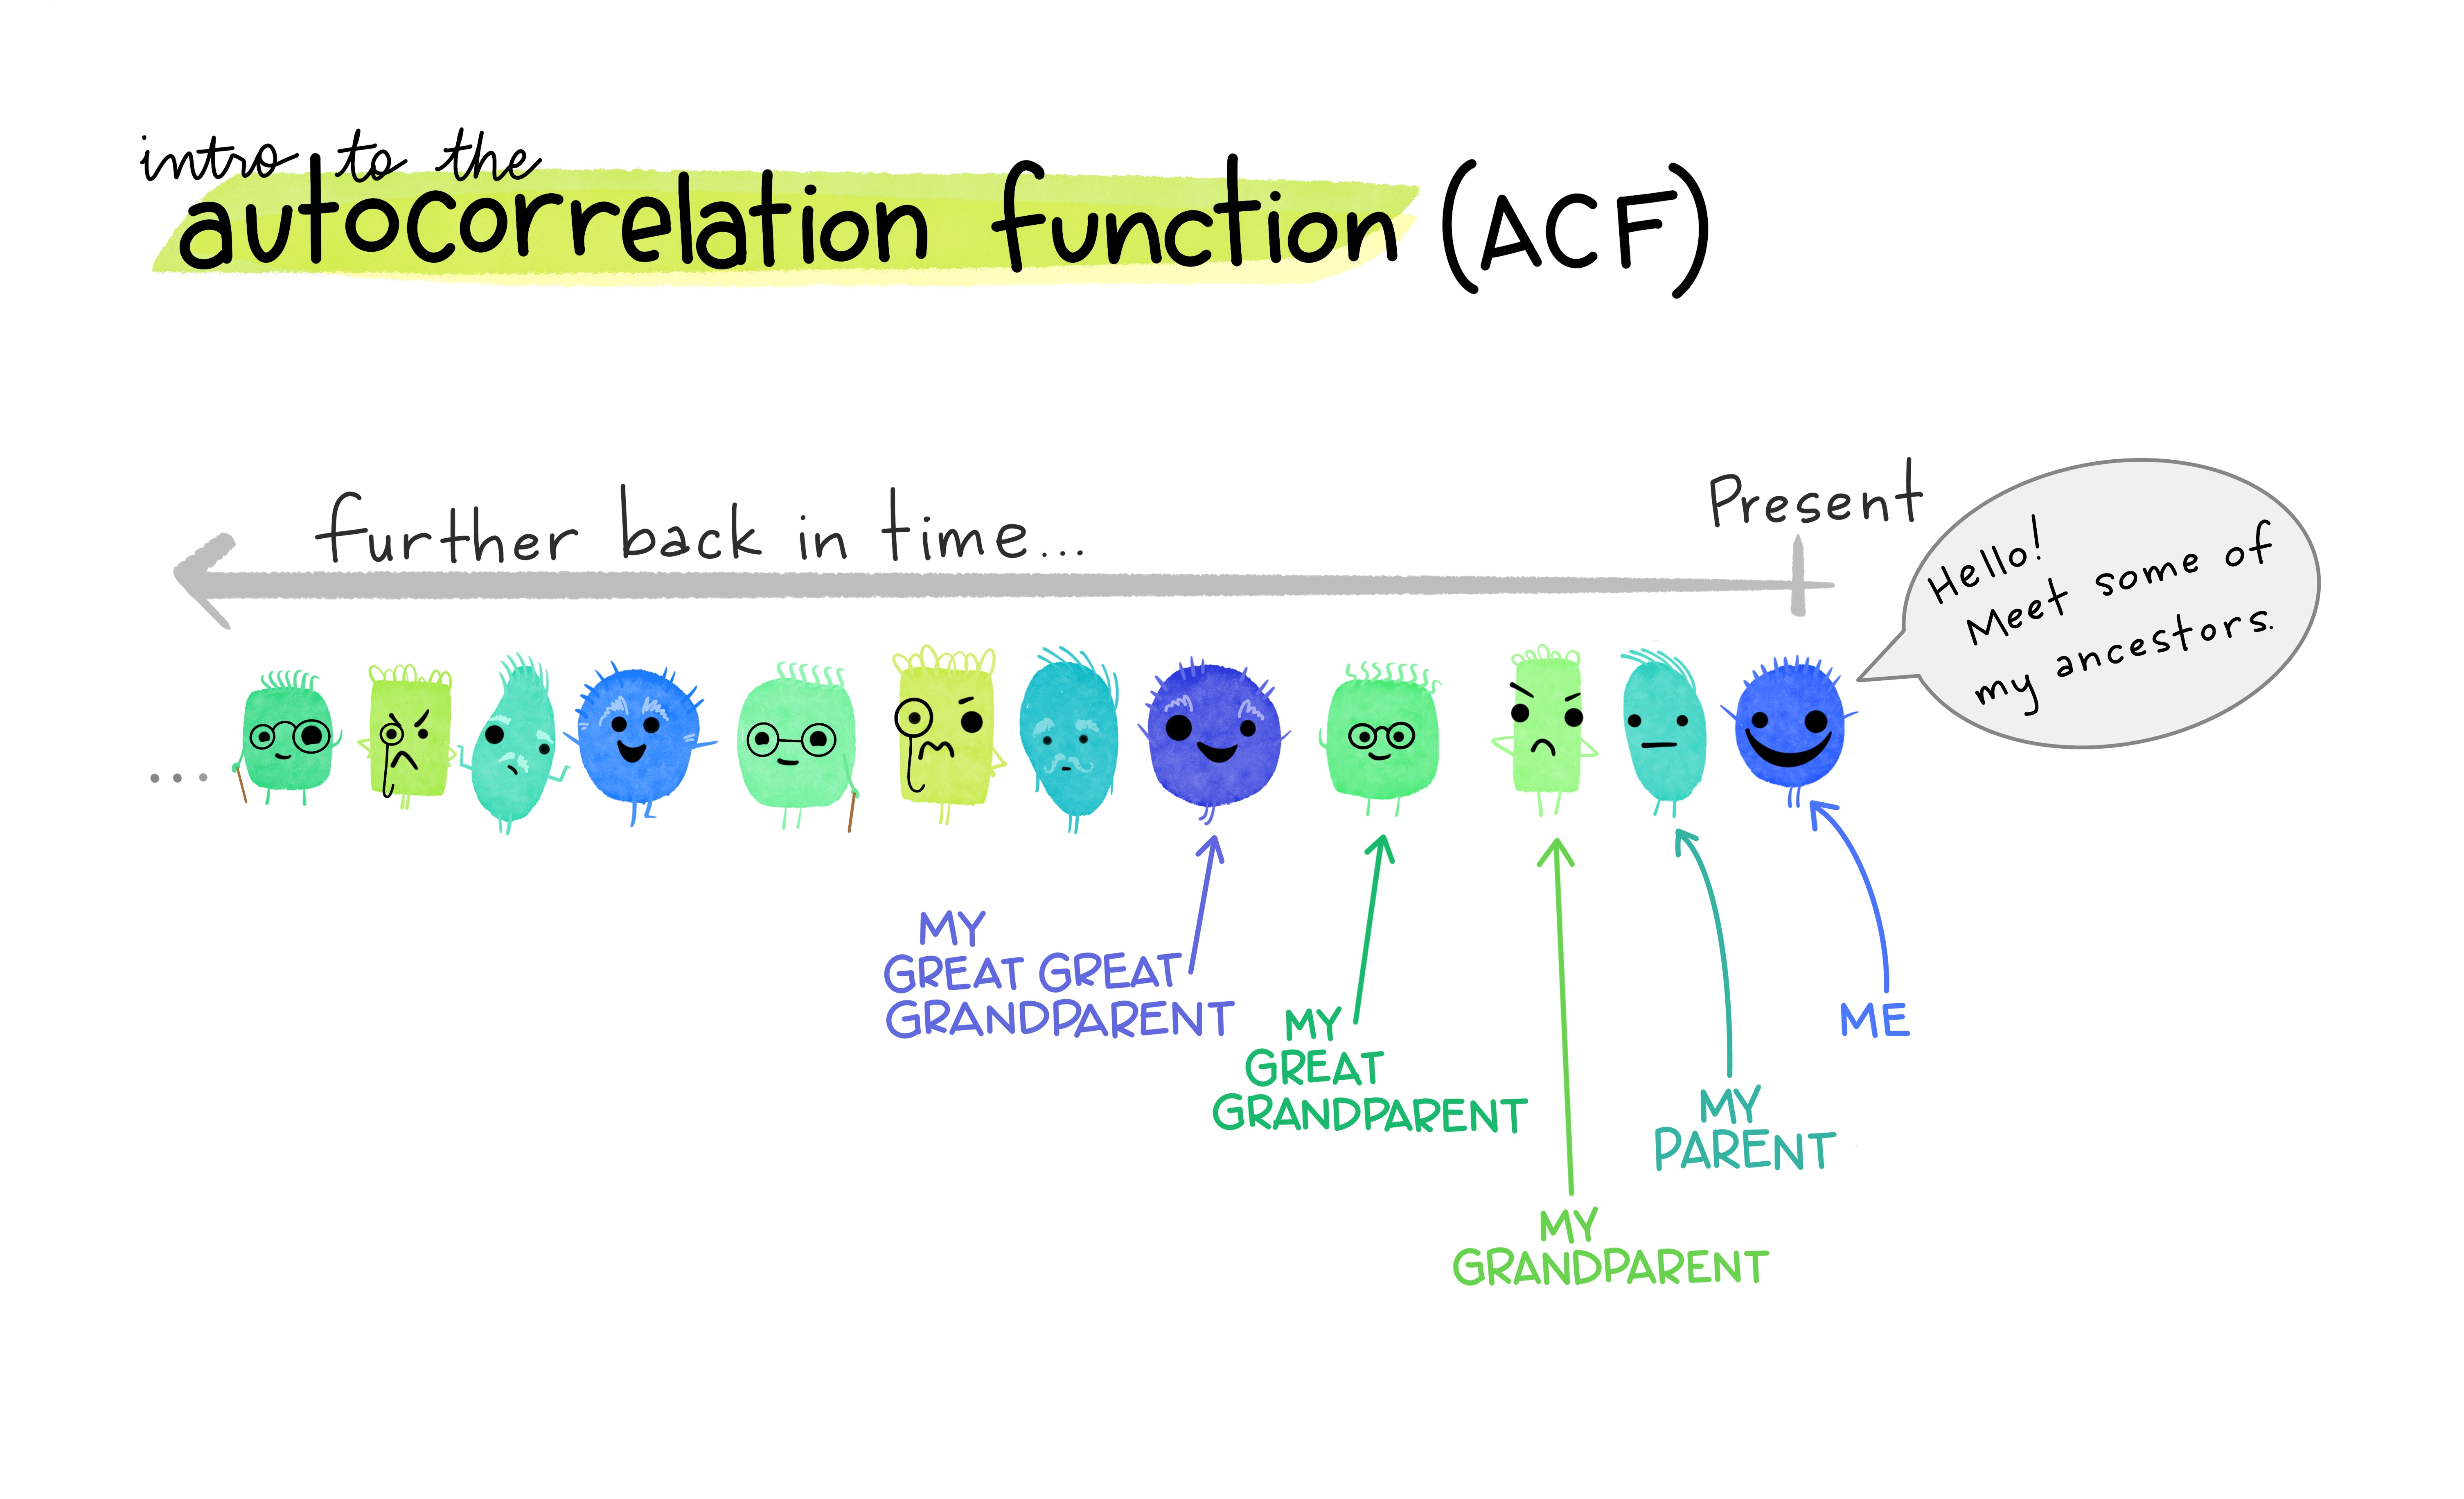
\includegraphics[width=19cm, height=7.4cm]{acf_1}}
\only<2>{\centering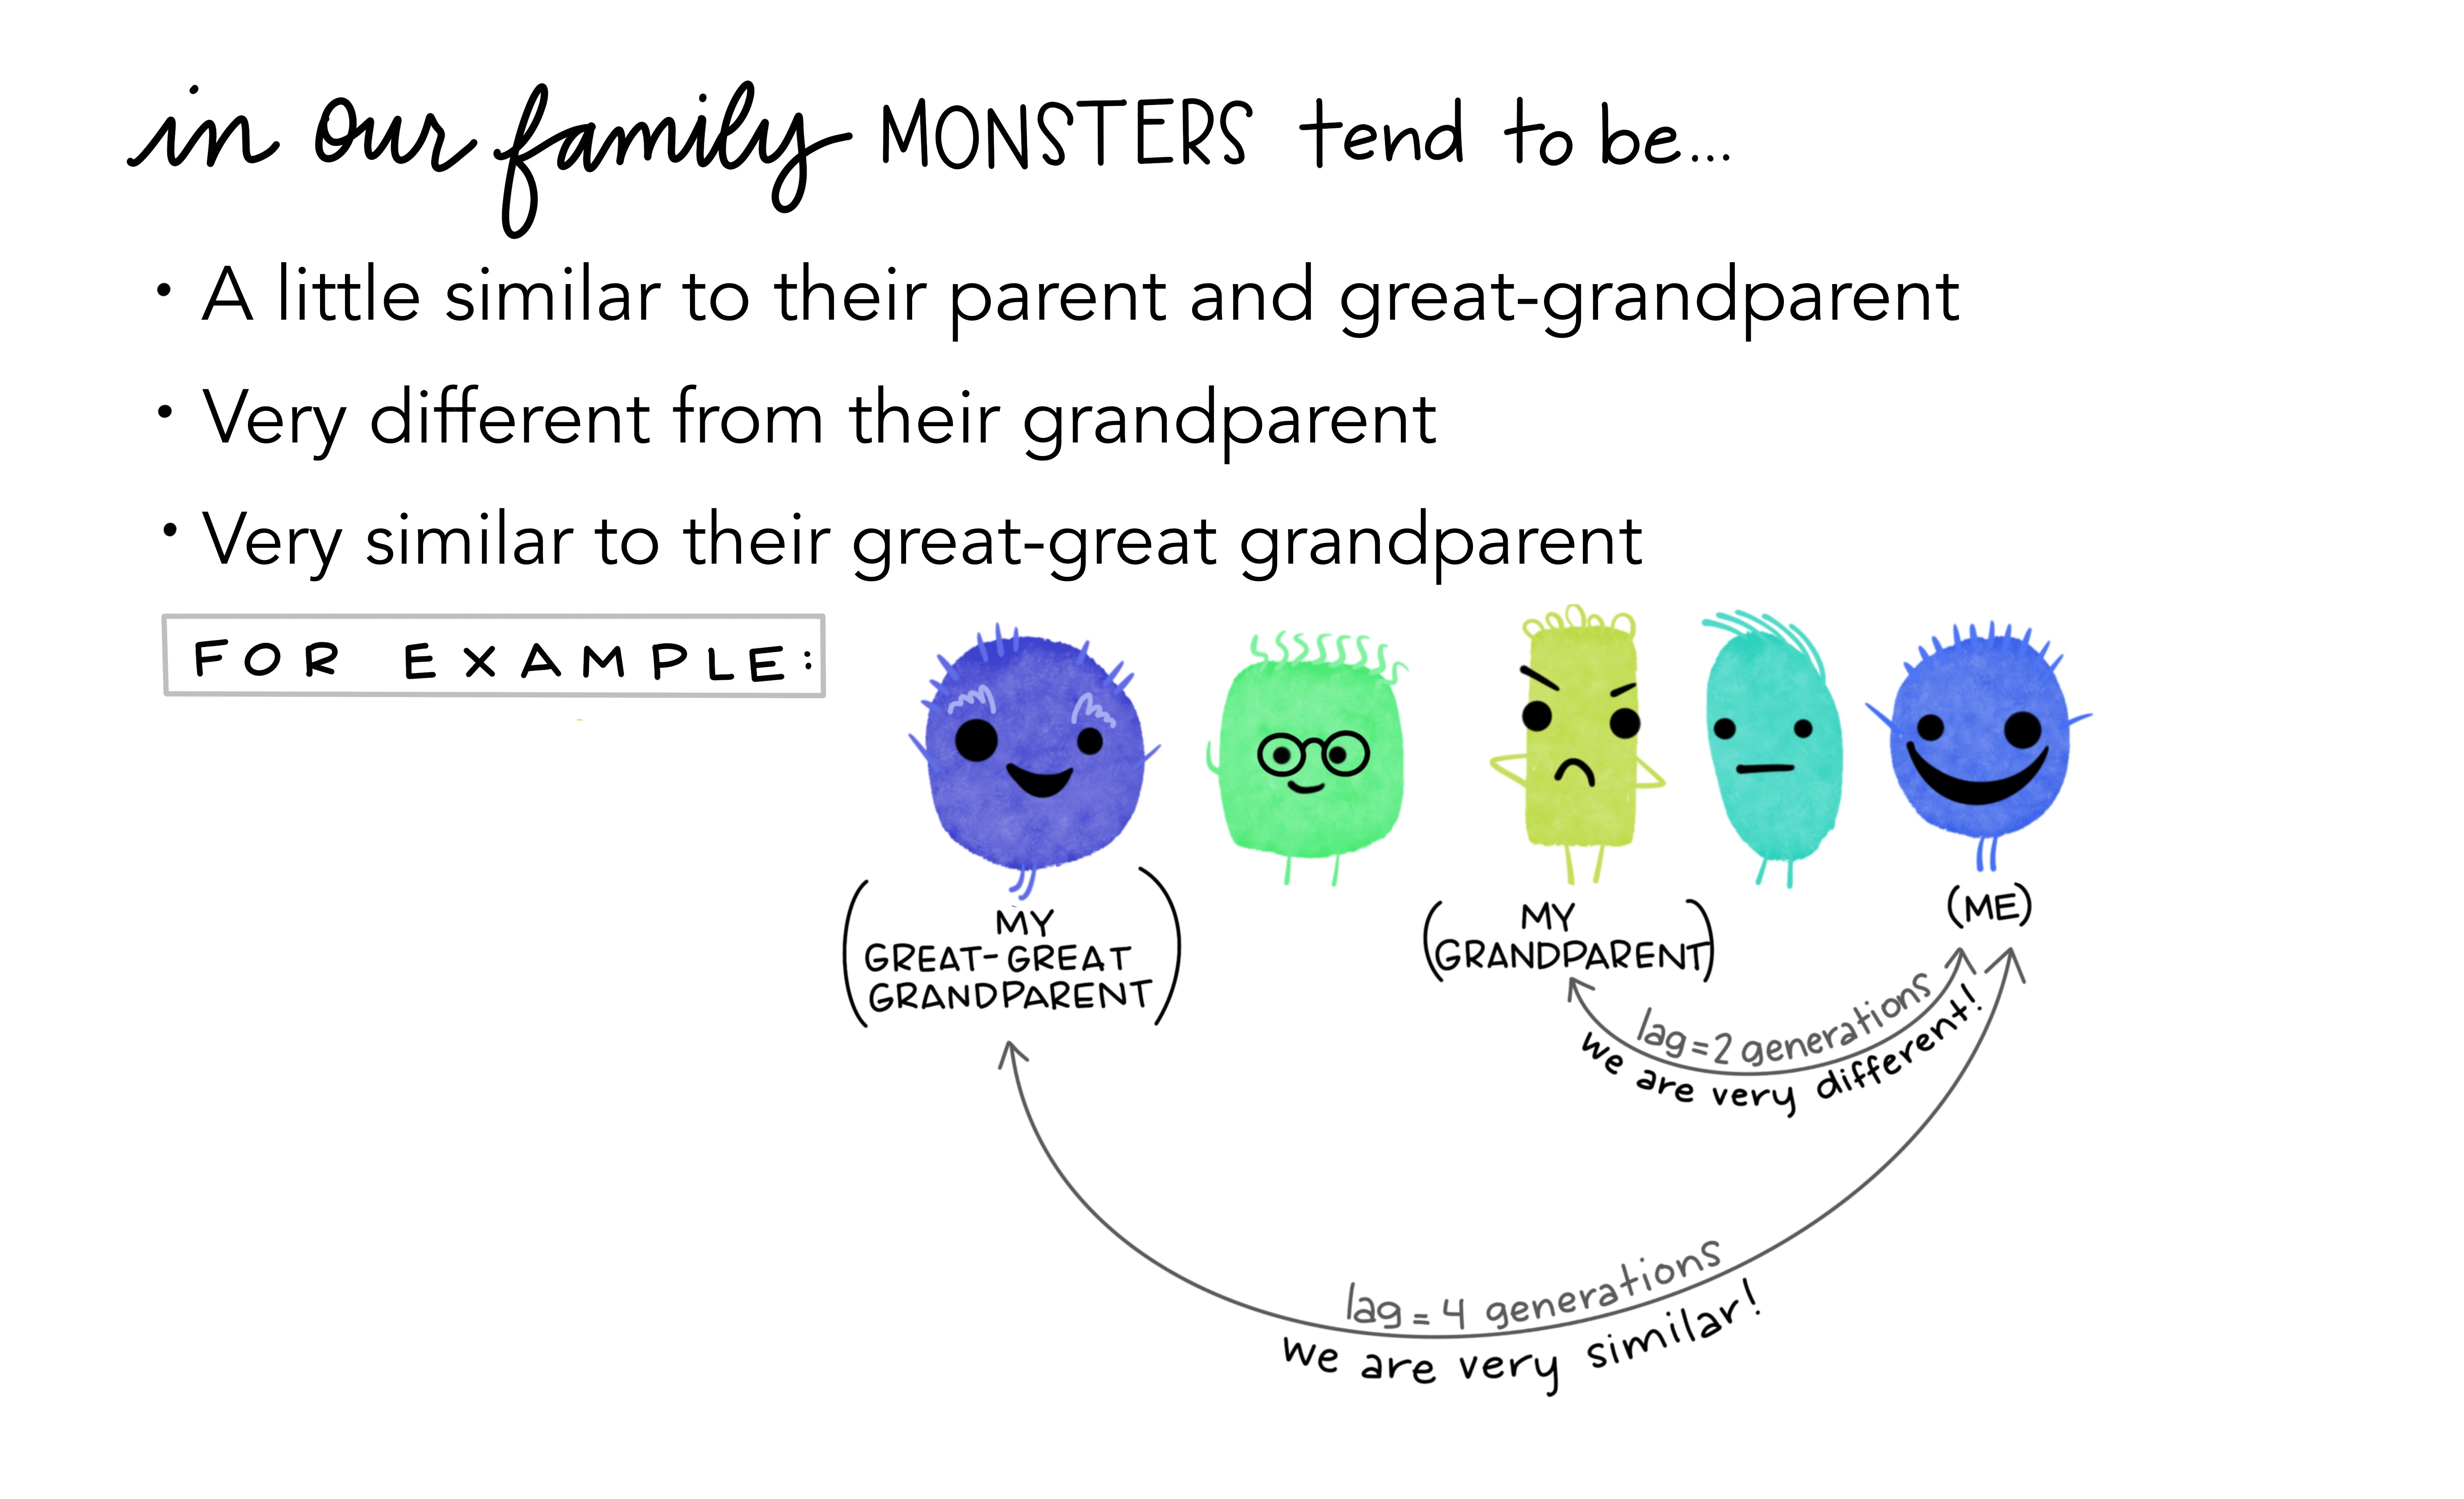
\includegraphics[width=19cm, height=7.4cm]{acf_2}}
\only<3>{\centering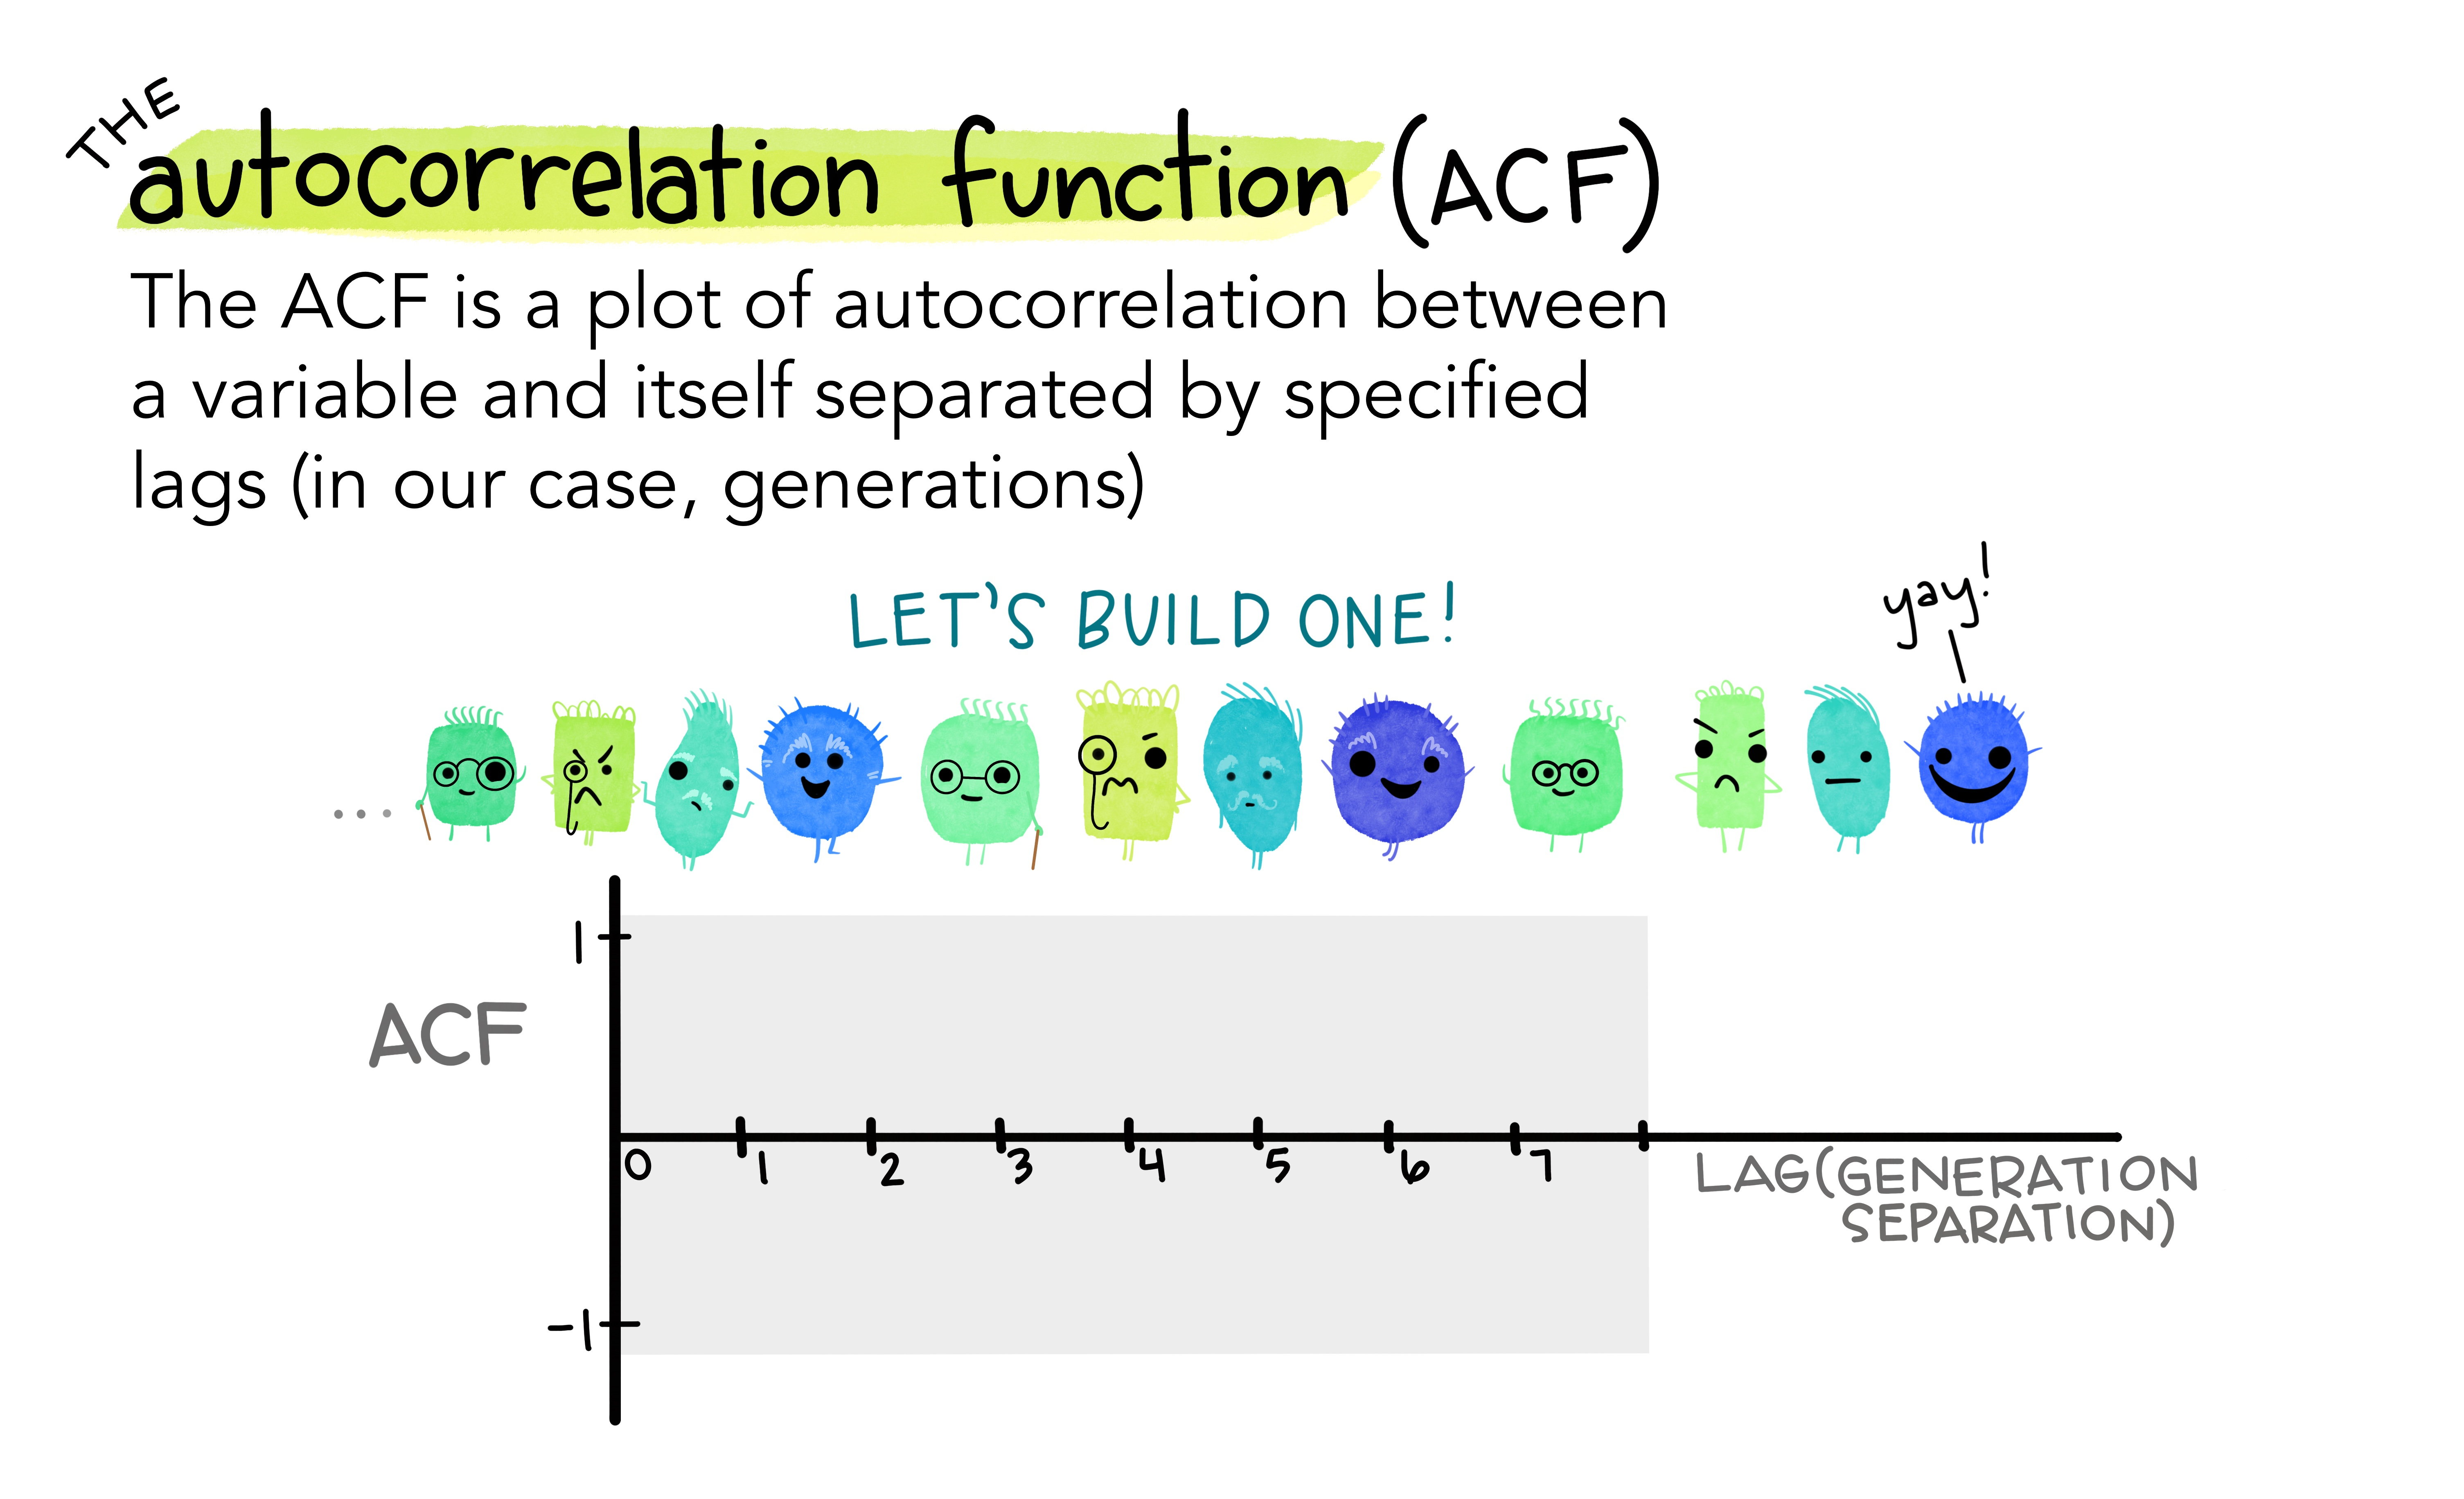
\includegraphics[width=19cm, height=7.4cm]{acf_3}}
\only<4>{\centering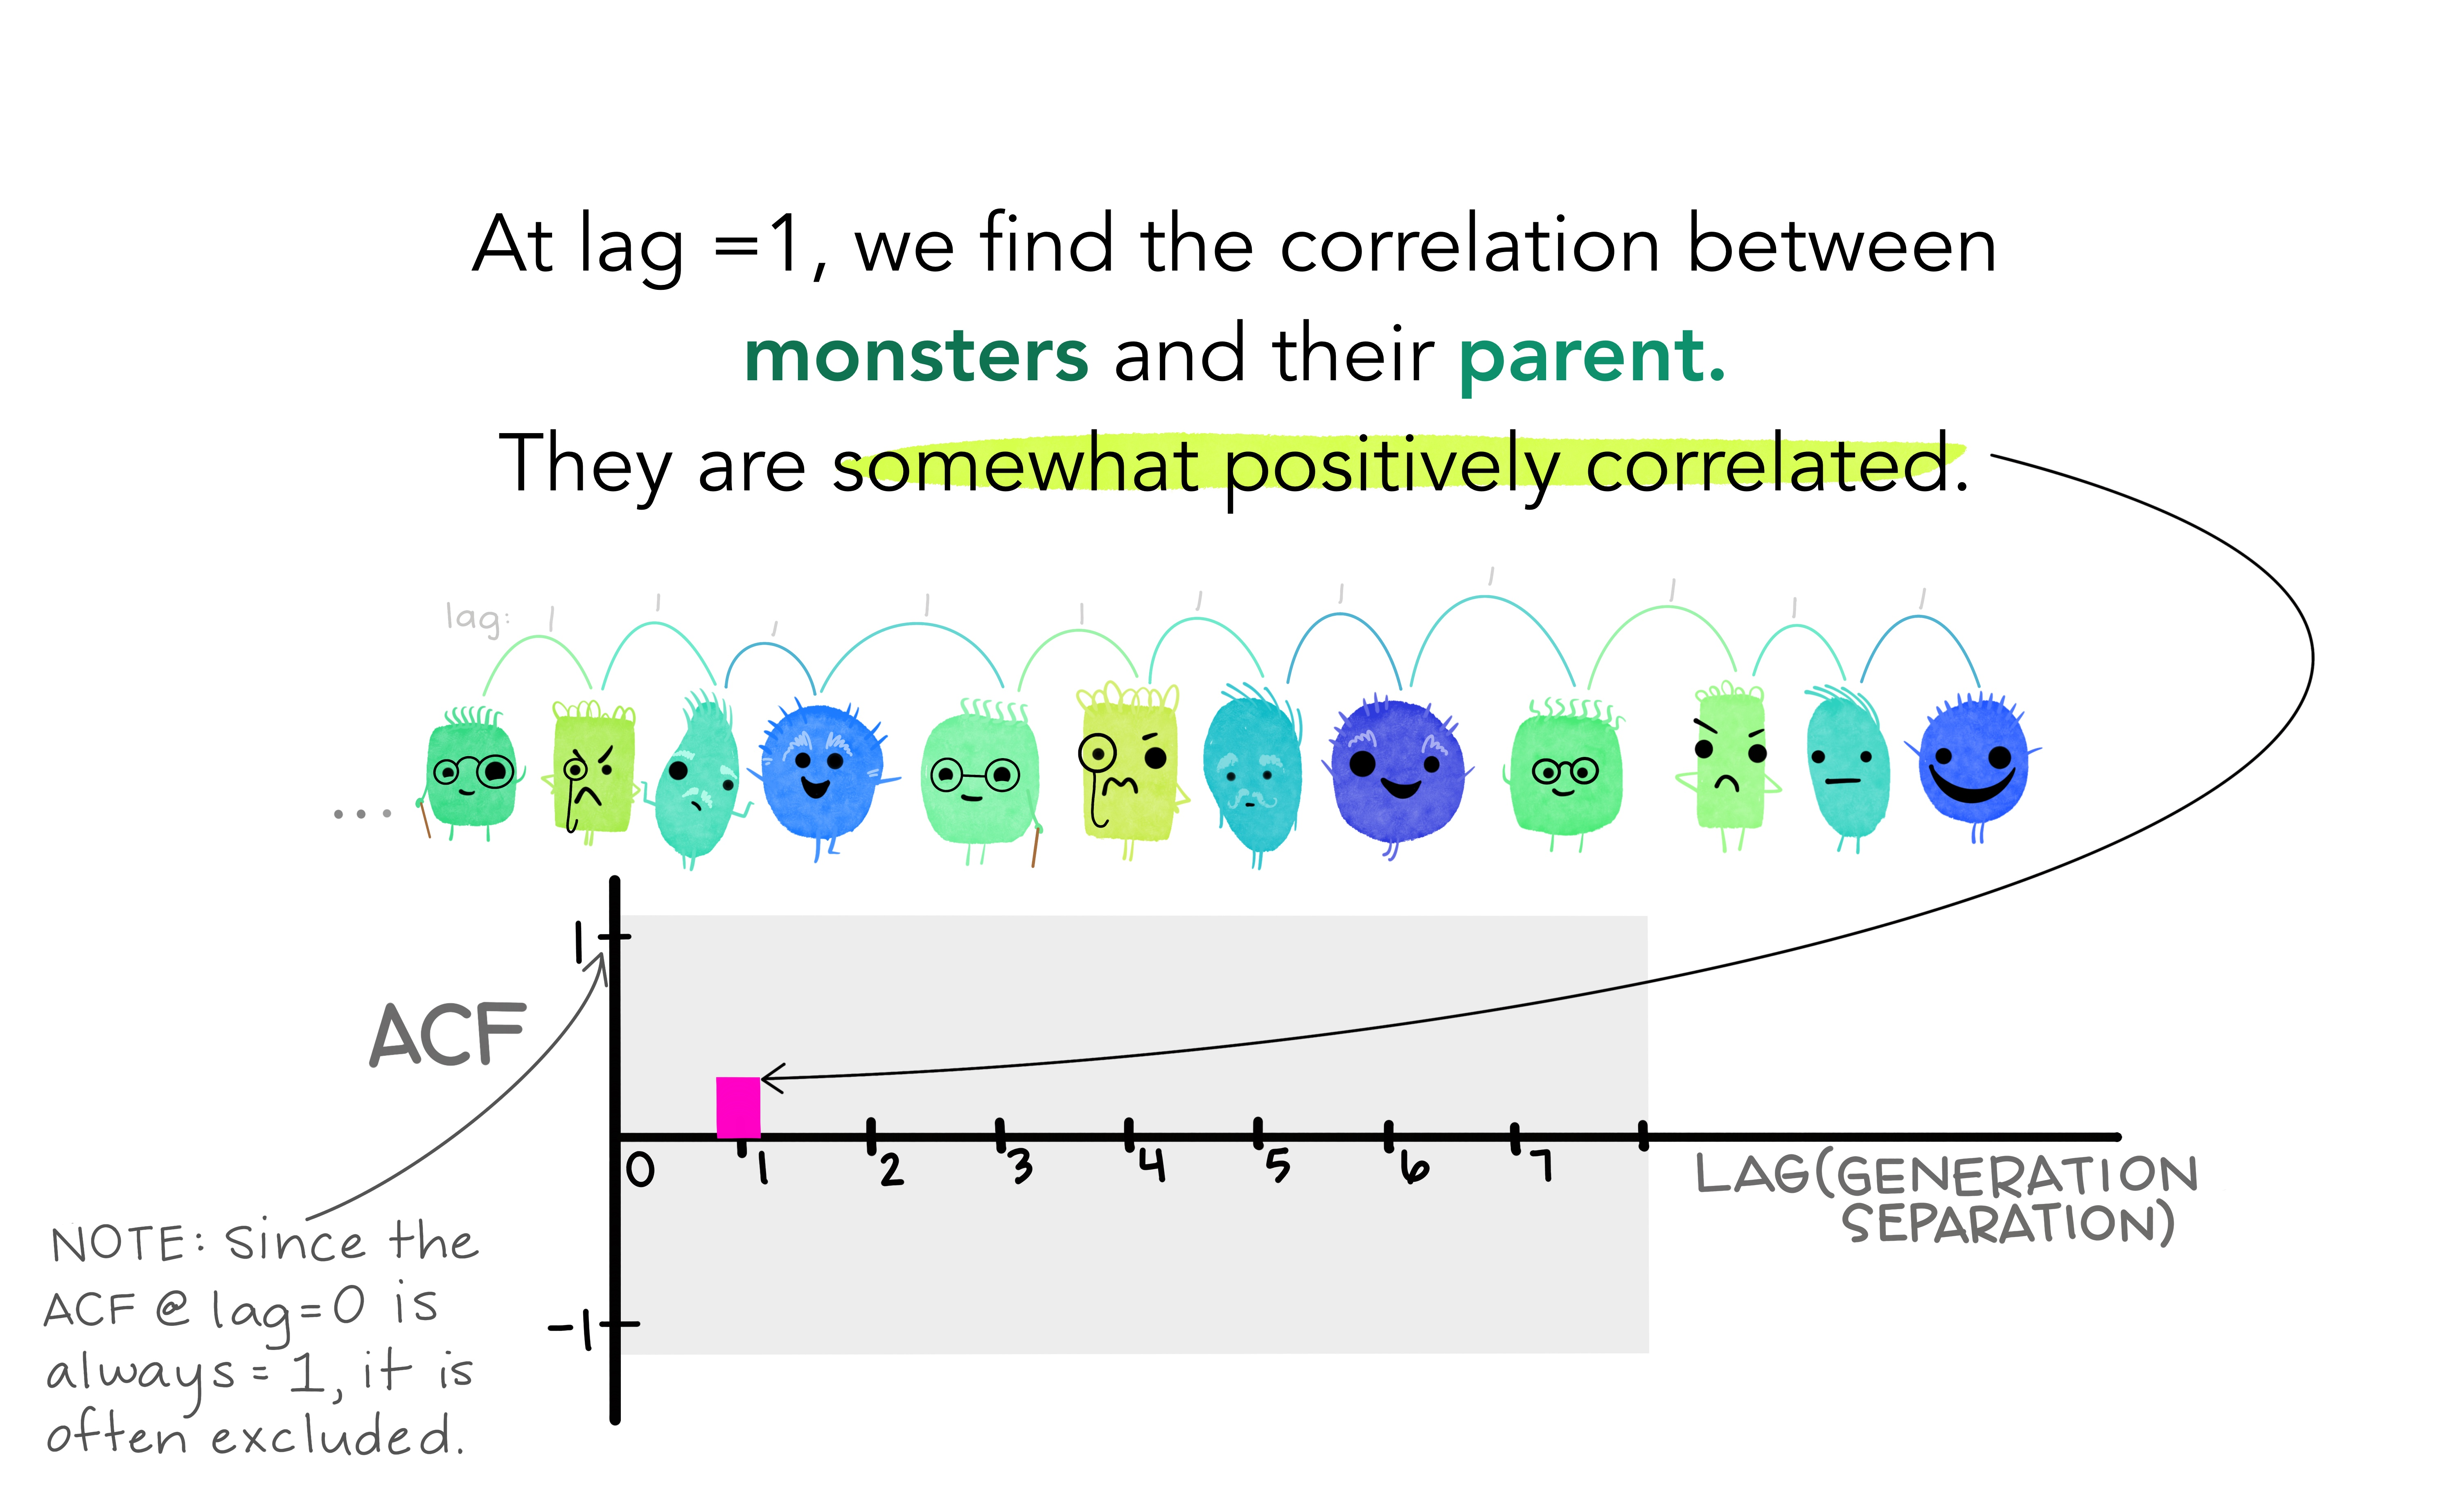
\includegraphics[width=19cm, height=7.4cm]{acf_4}}
\only<5>{\centering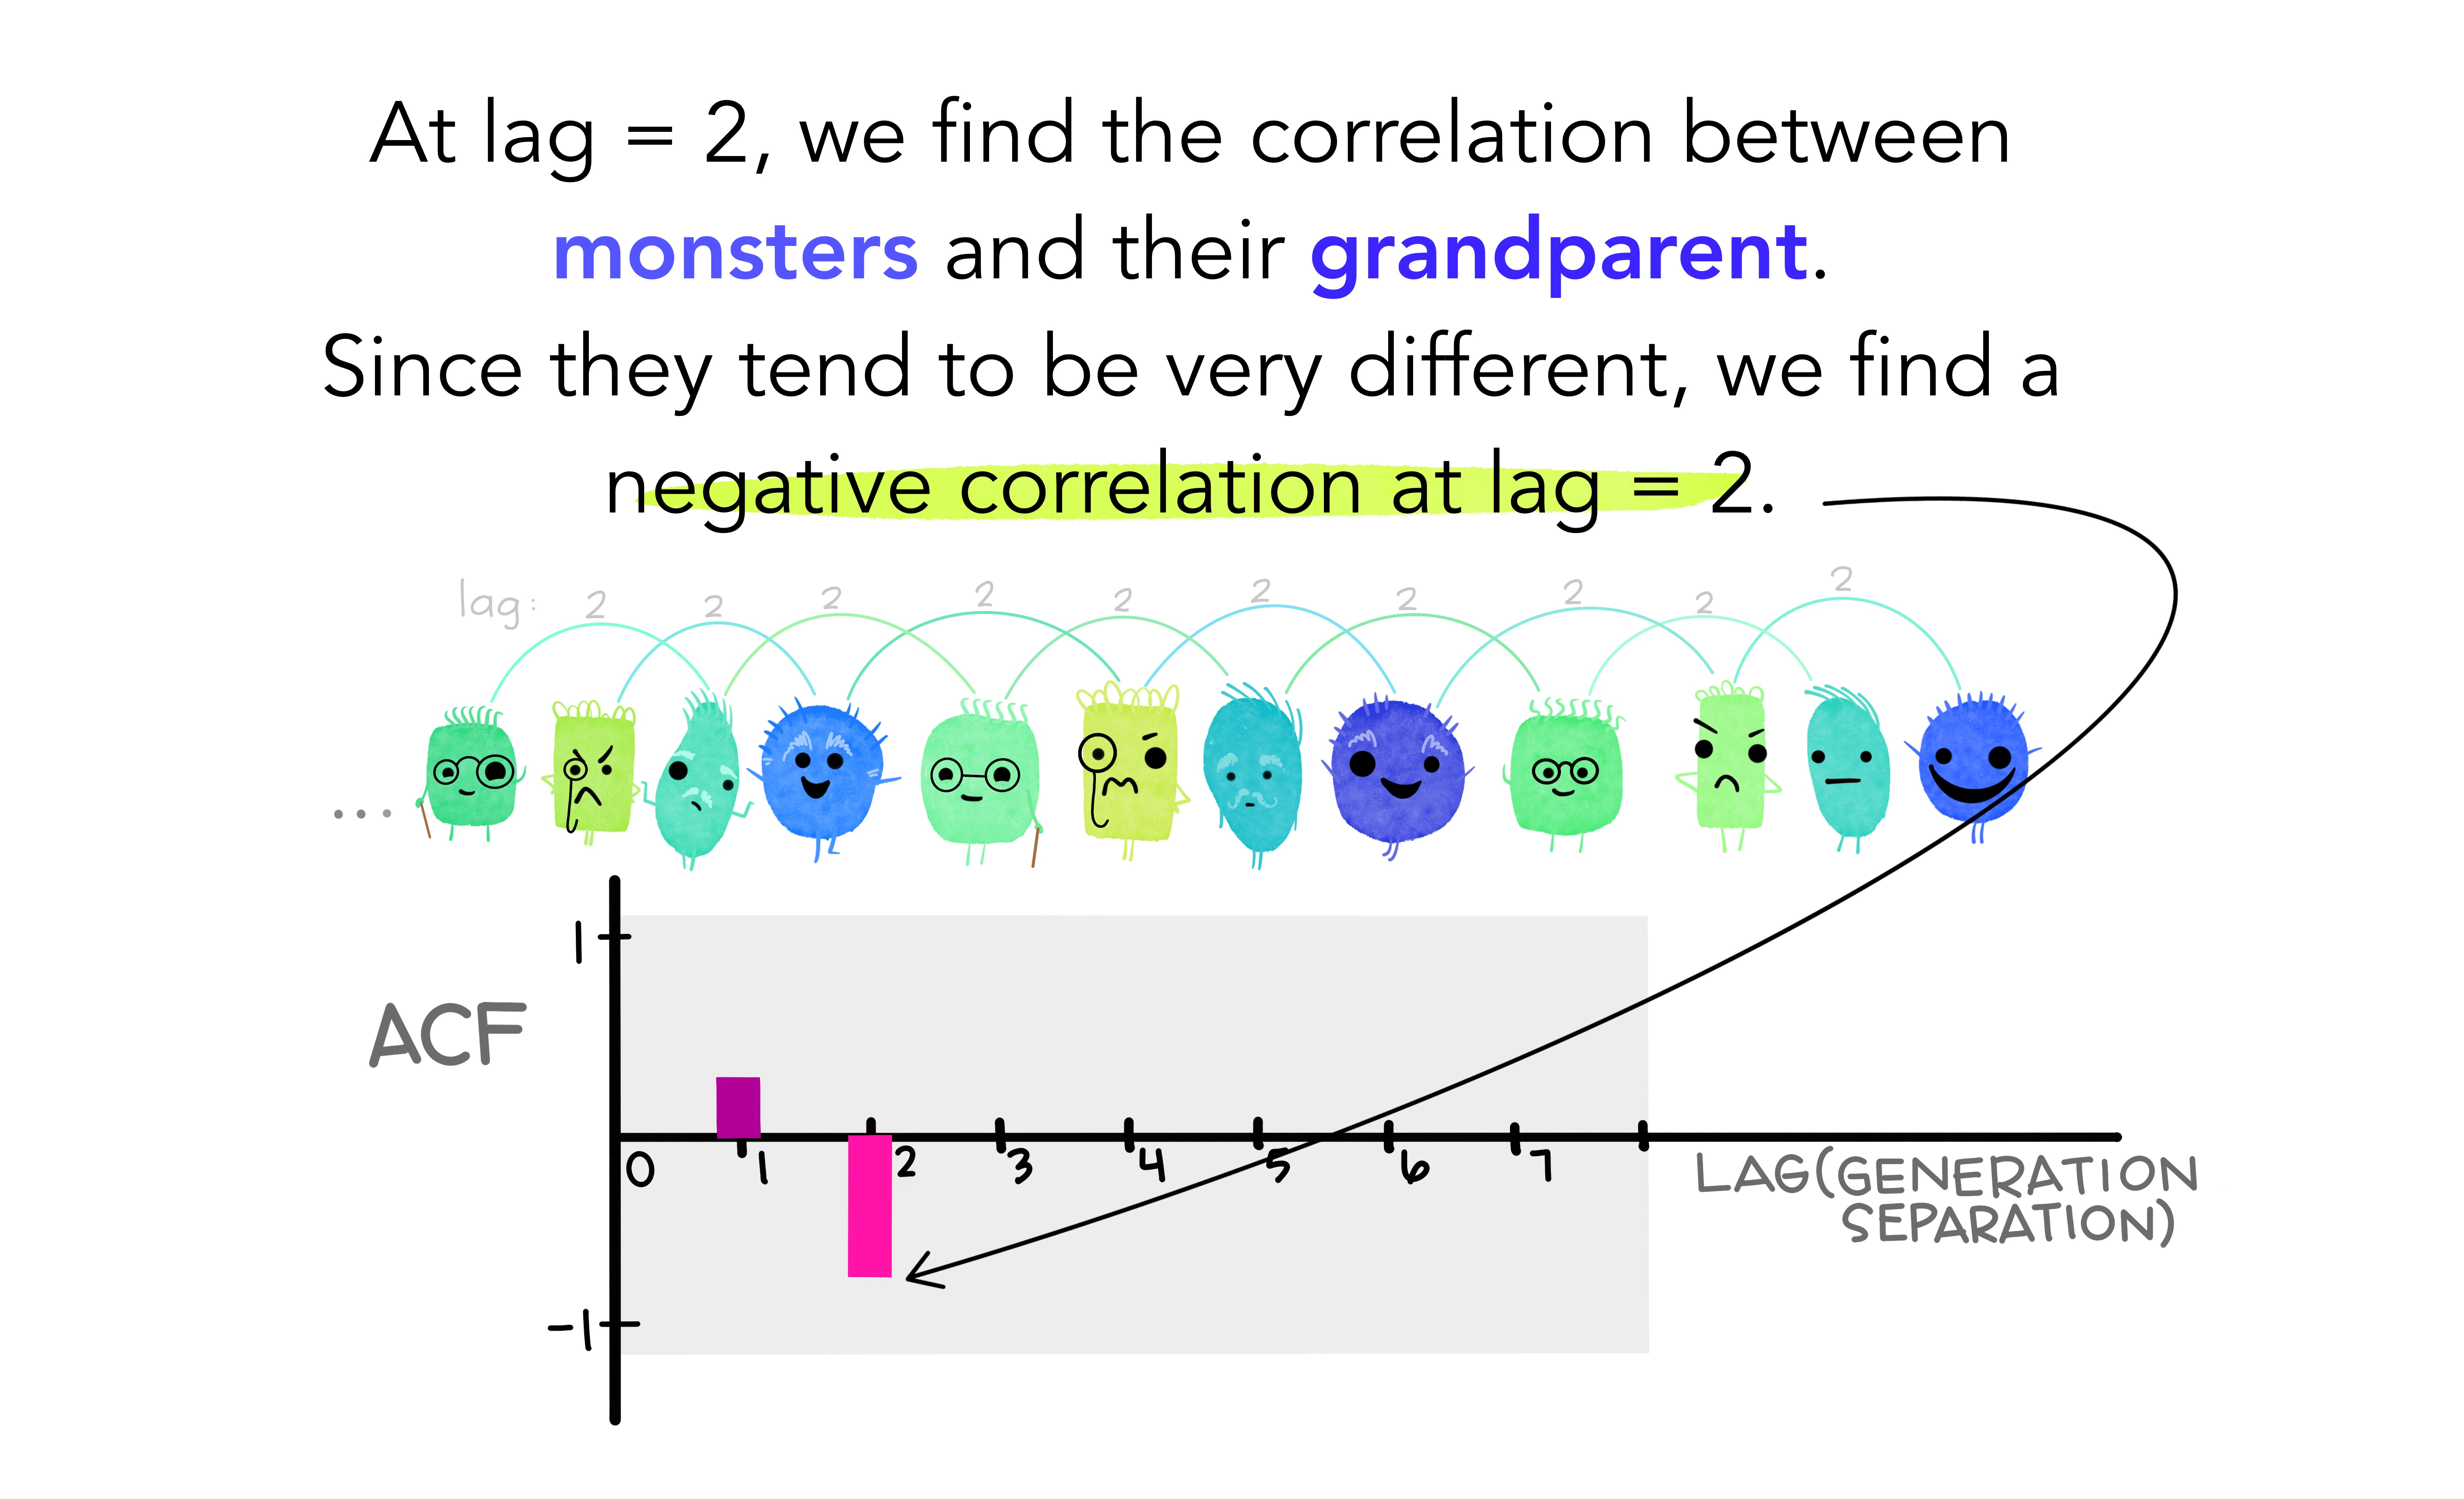
\includegraphics[width=19cm, height=7.4cm]{acf_5}}
\only<6>{\centering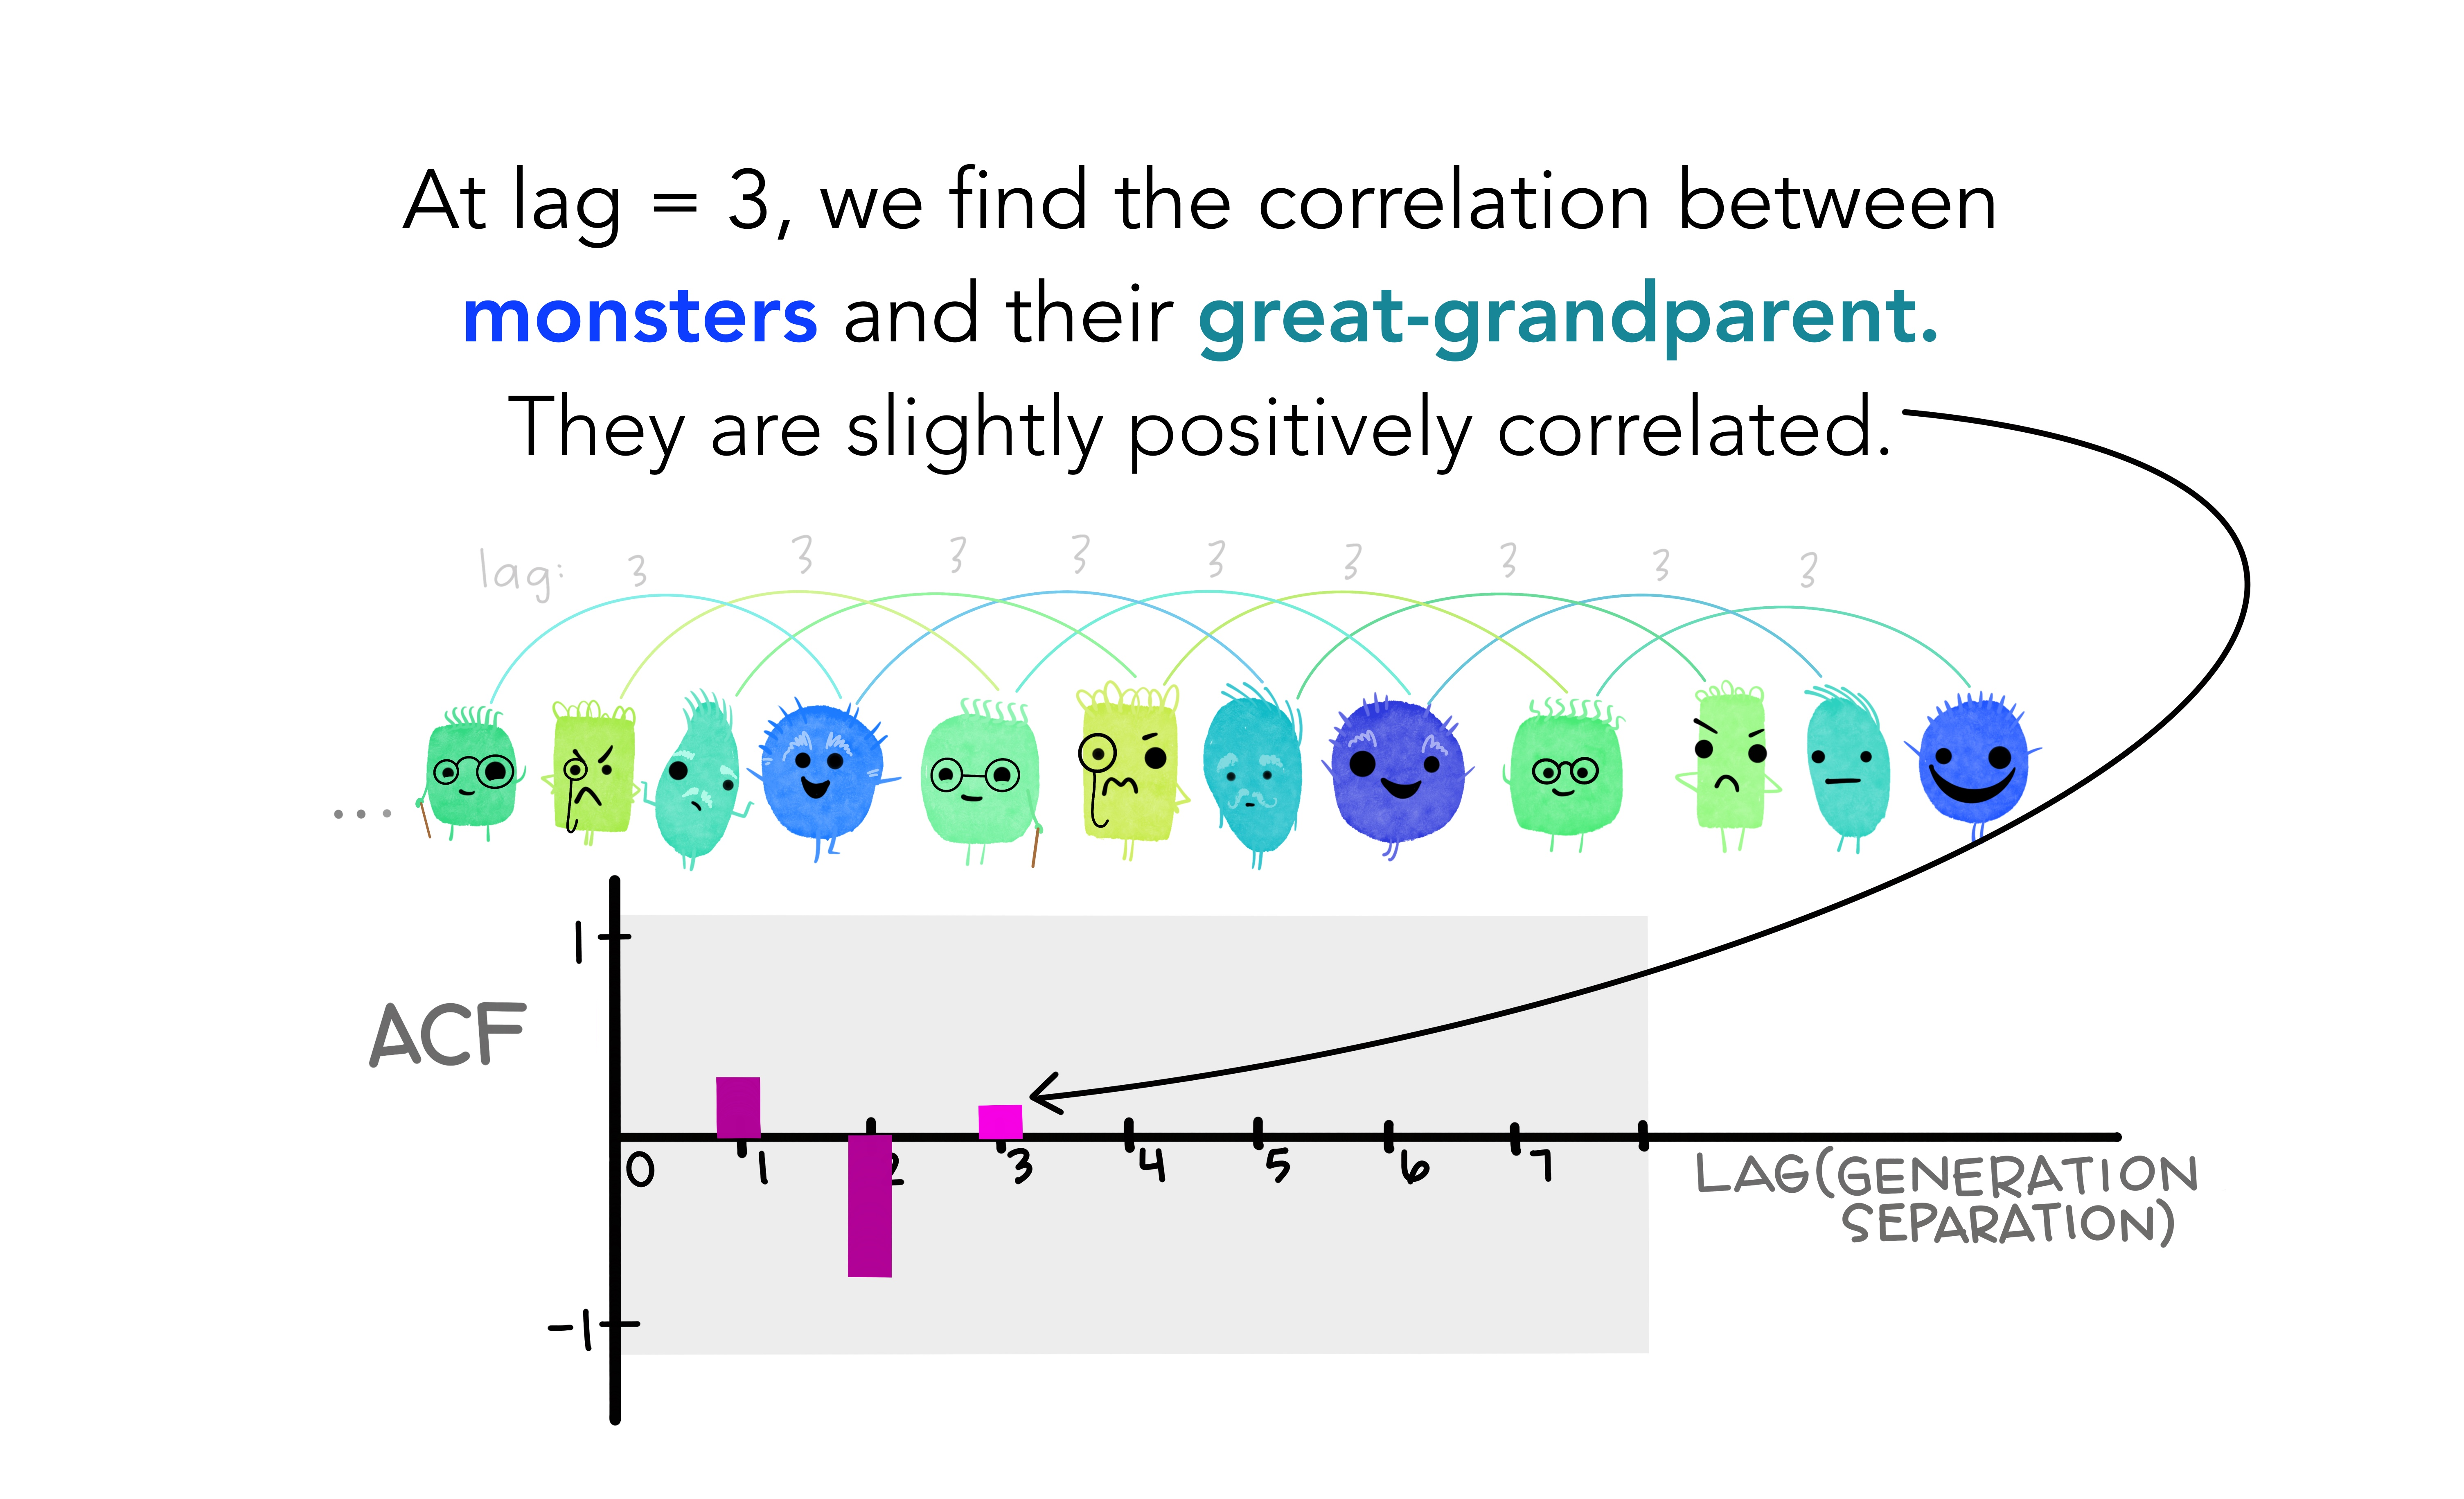
\includegraphics[width=19cm, height=7.4cm]{acf_6}}
\only<7>{\centering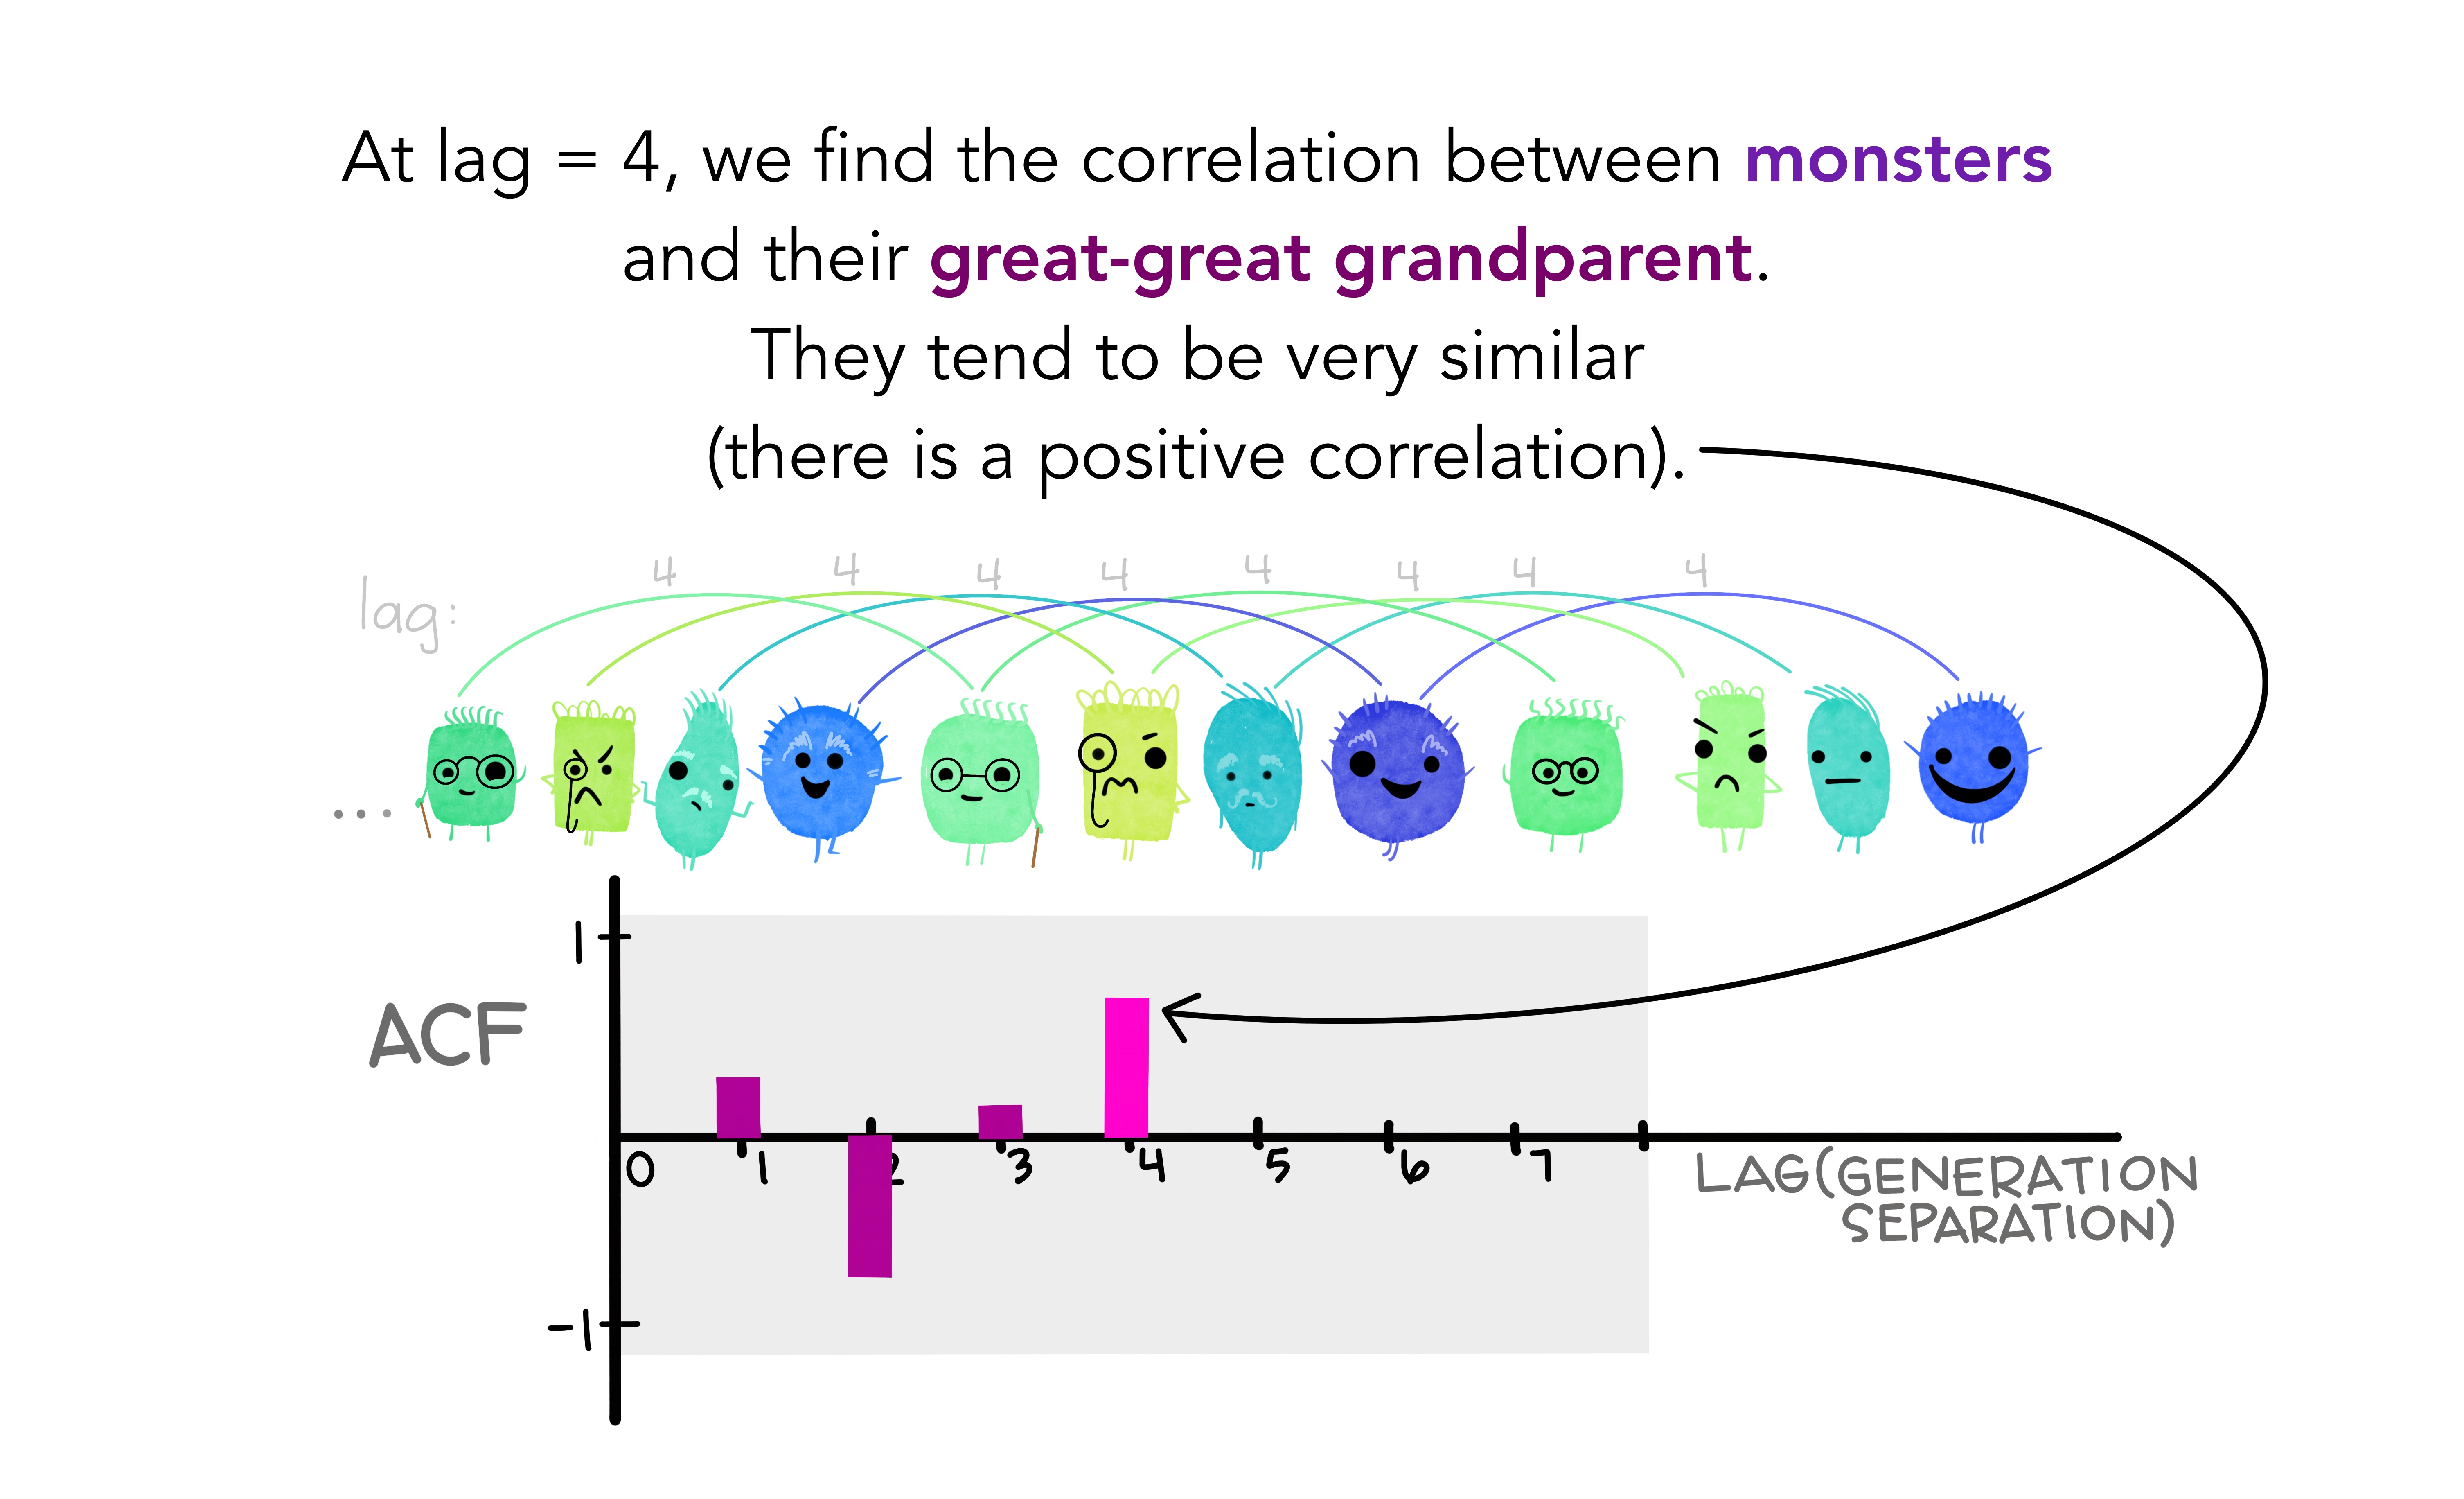
\includegraphics[width=19cm, height=7.4cm]{acf_7}}
\only<8>{\centering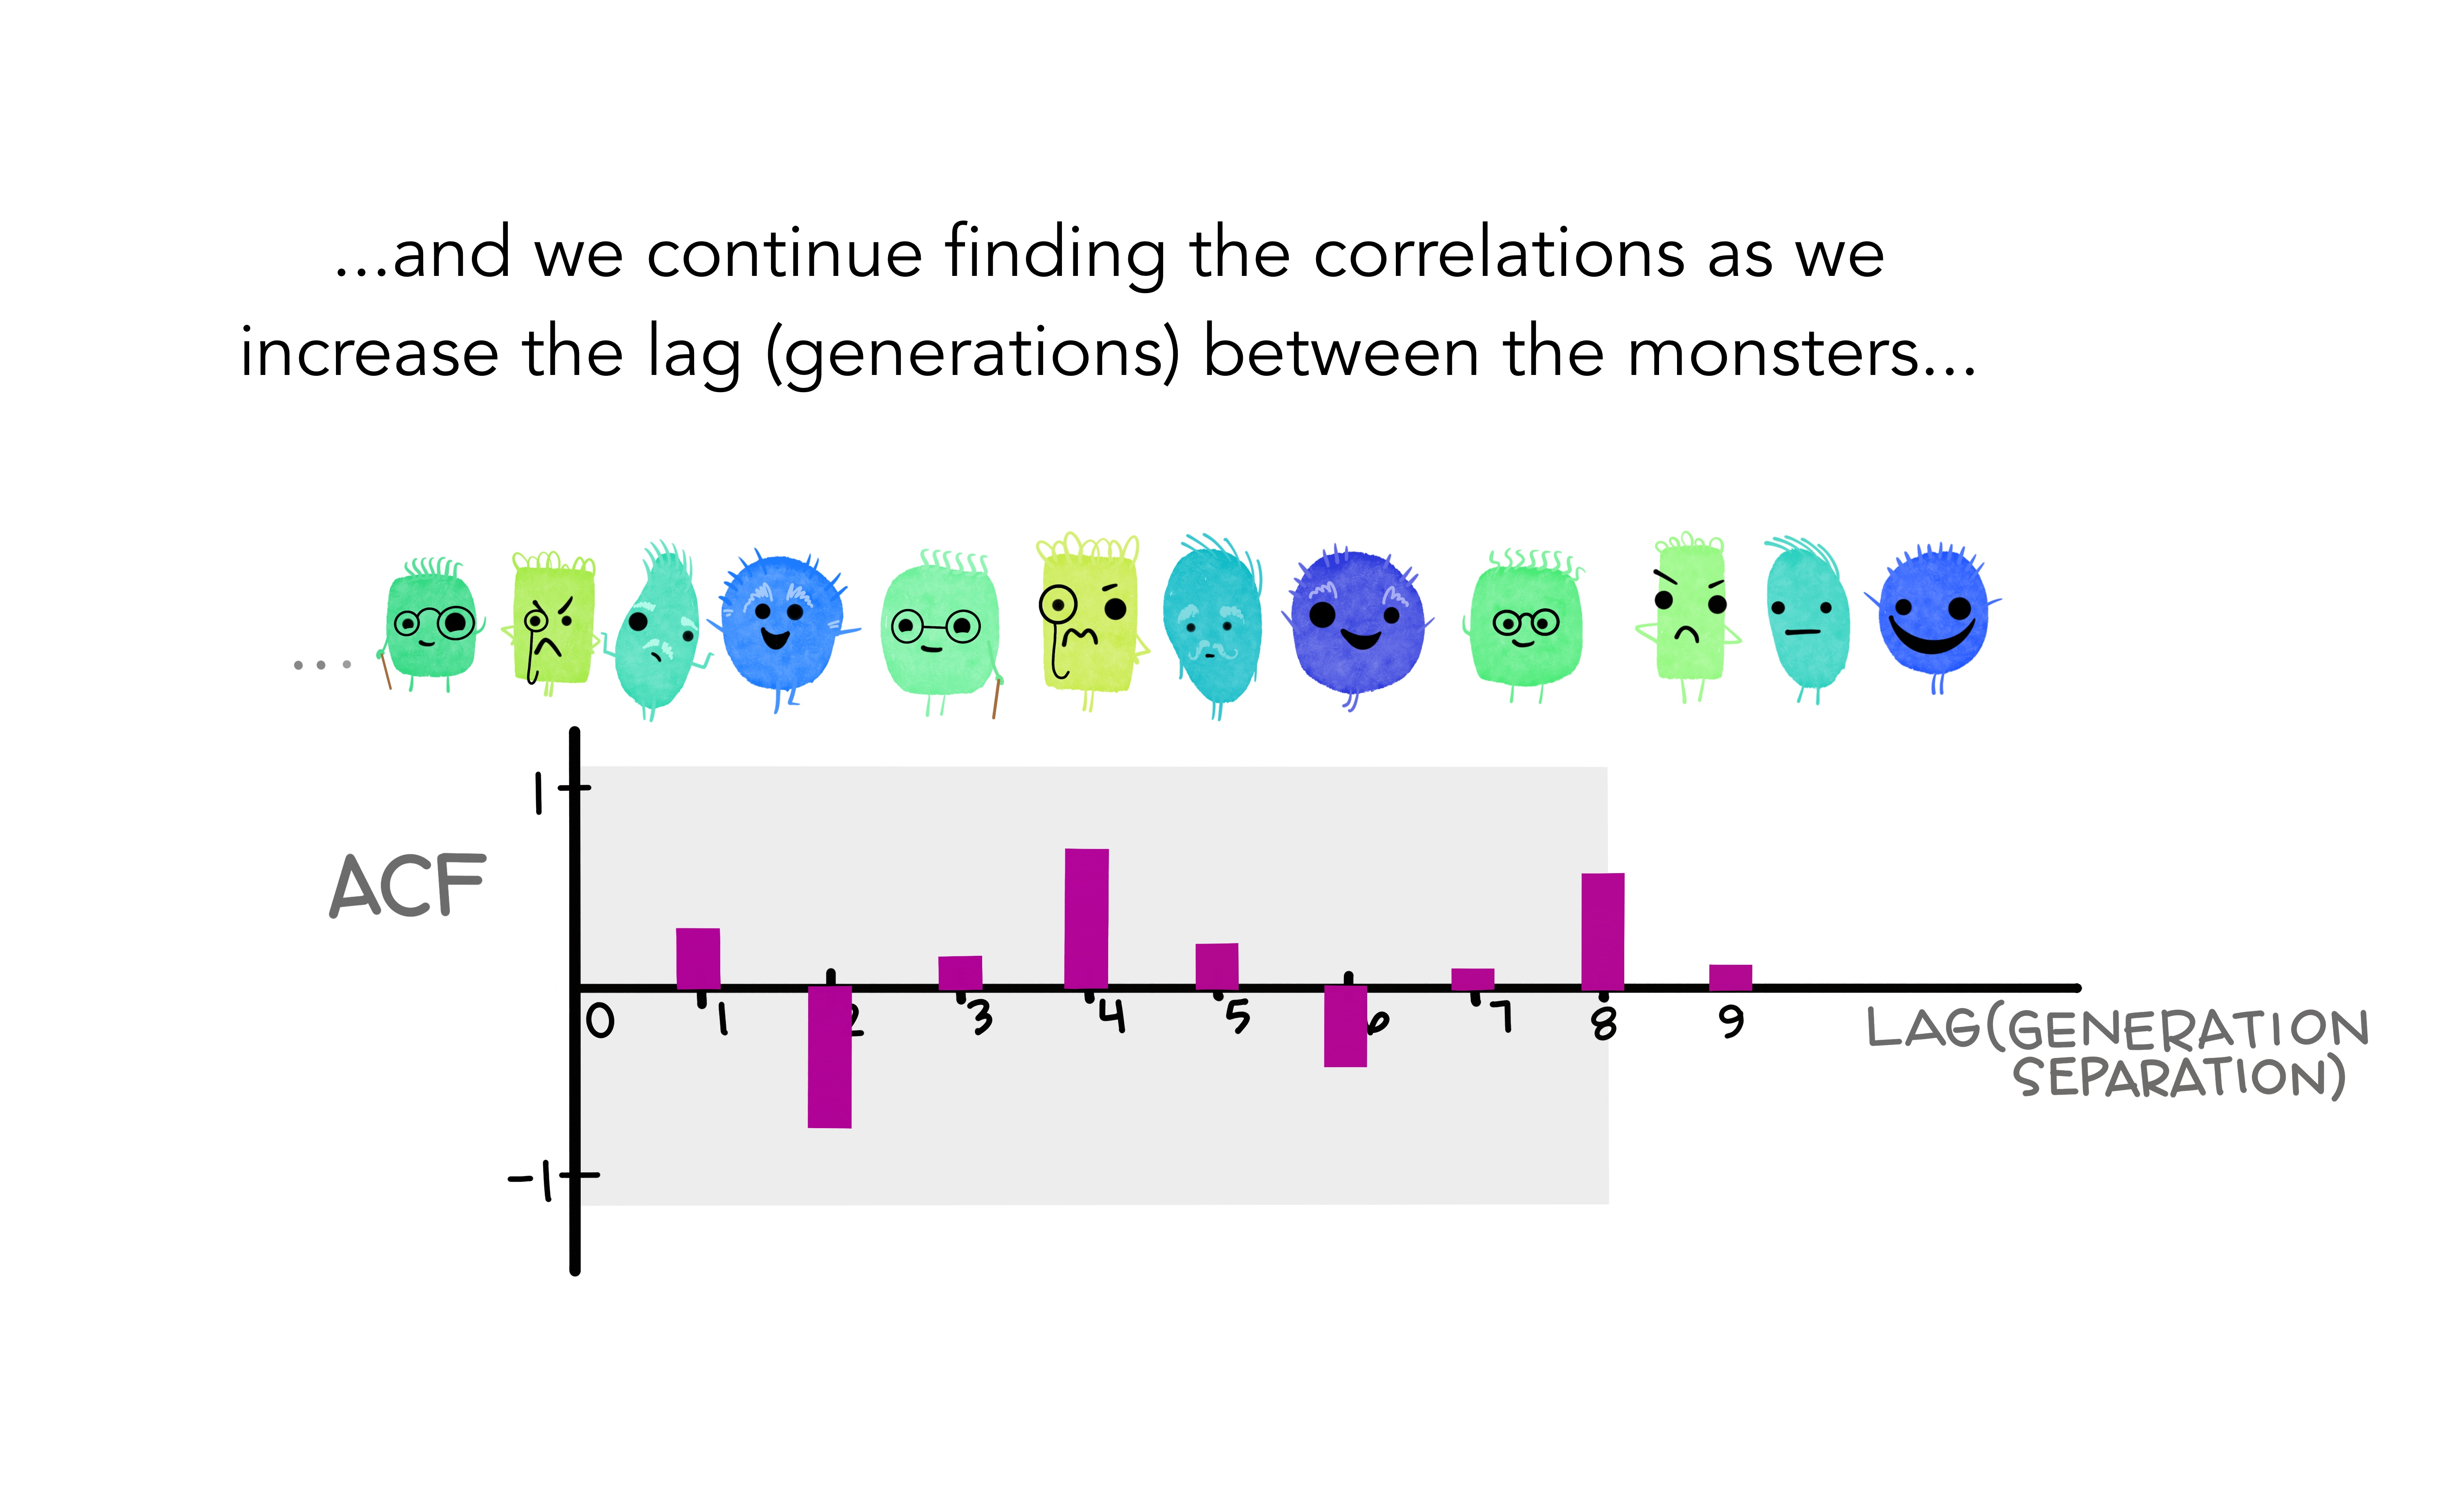
\includegraphics[width=19cm, height=7.4cm]{acf_8}}
\only<9>{\centering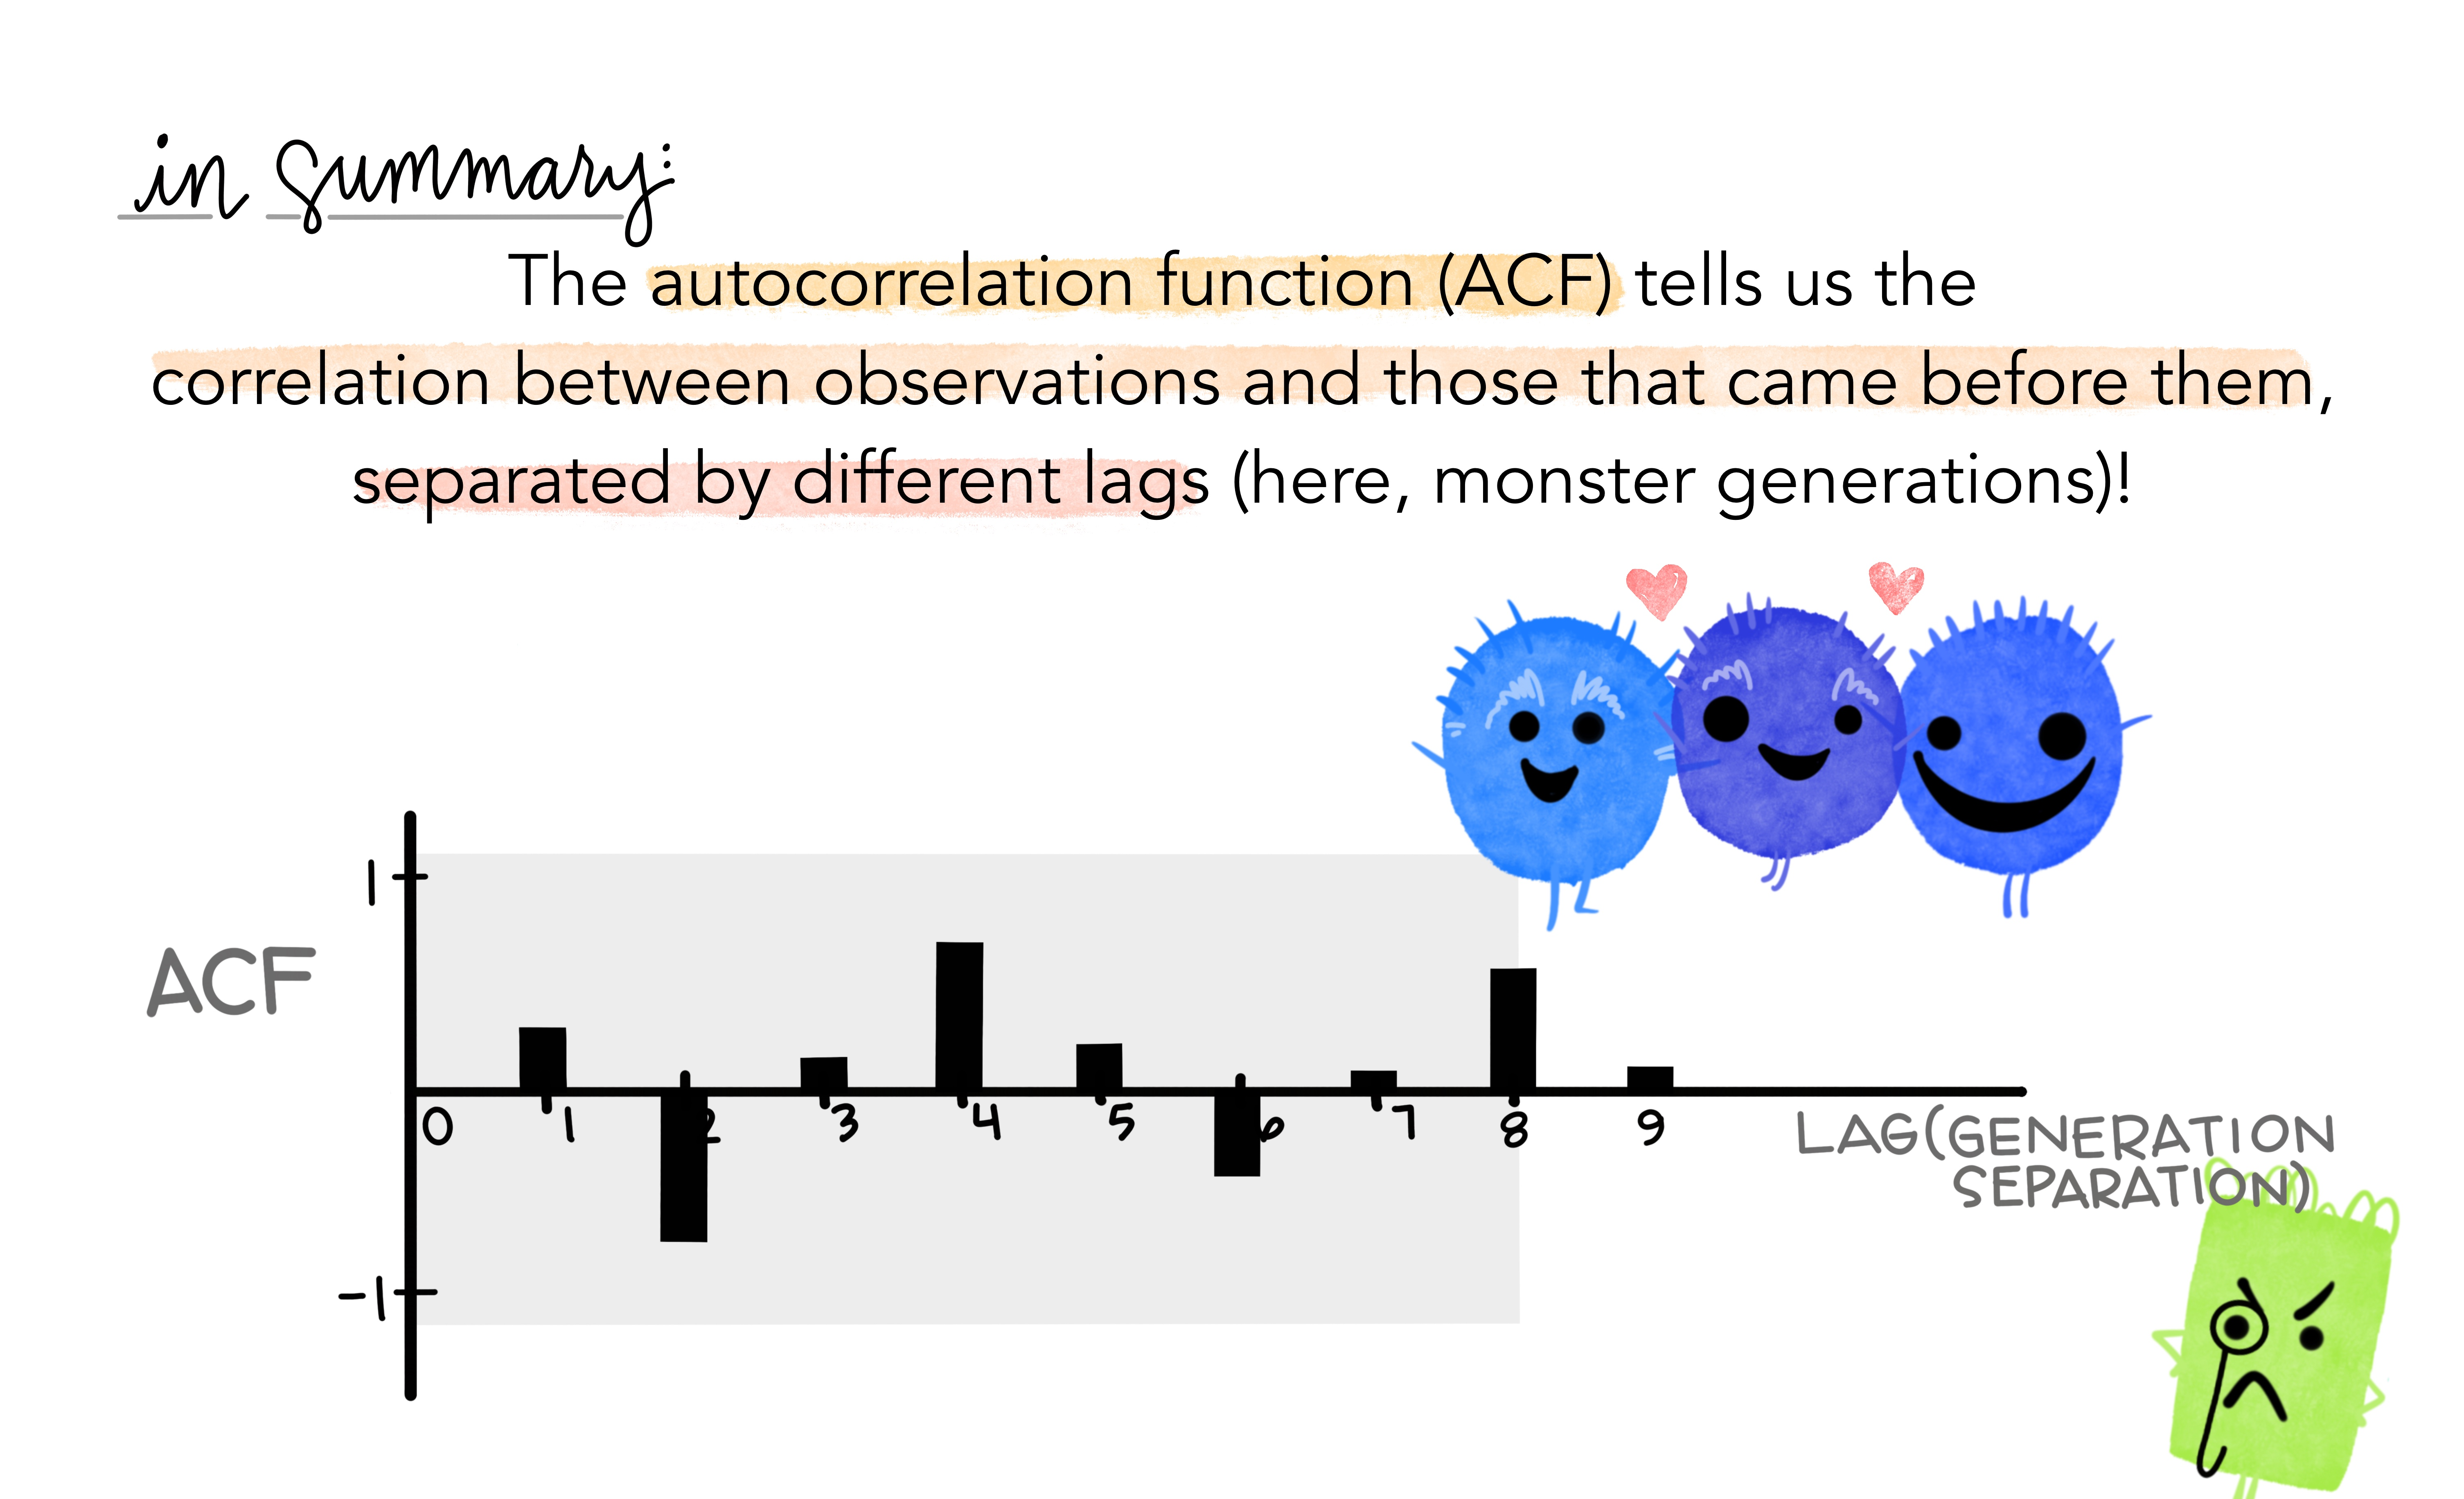
\includegraphics[width=19cm, height=7.4cm]{acf_9}}

\vspace*{10cm}

\begin{textblock}{3}(0.3,8.7)\fontsize{7}{9}\sf
Artwork by @allison\_horst
\end{textblock}
\end{frame}

\begin{frame}[fragile]{US retail trade employment}
\protect\hypertarget{us-retail-trade-employment}{}
\fontsize{10}{10}\sf

\begin{Shaded}
\begin{Highlighting}[]
\NormalTok{retail }\OtherTok{\textless{}{-}}\NormalTok{ us\_employment }\SpecialCharTok{\%\textgreater{}\%}
  \FunctionTok{filter}\NormalTok{(Title }\SpecialCharTok{==} \StringTok{"Retail Trade"}\NormalTok{, }\FunctionTok{year}\NormalTok{(Month) }\SpecialCharTok{\textgreater{}=} \DecValTok{1980}\NormalTok{)}
\NormalTok{retail }\SpecialCharTok{\%\textgreater{}\%} \FunctionTok{autoplot}\NormalTok{(Employed)}
\end{Highlighting}
\end{Shaded}

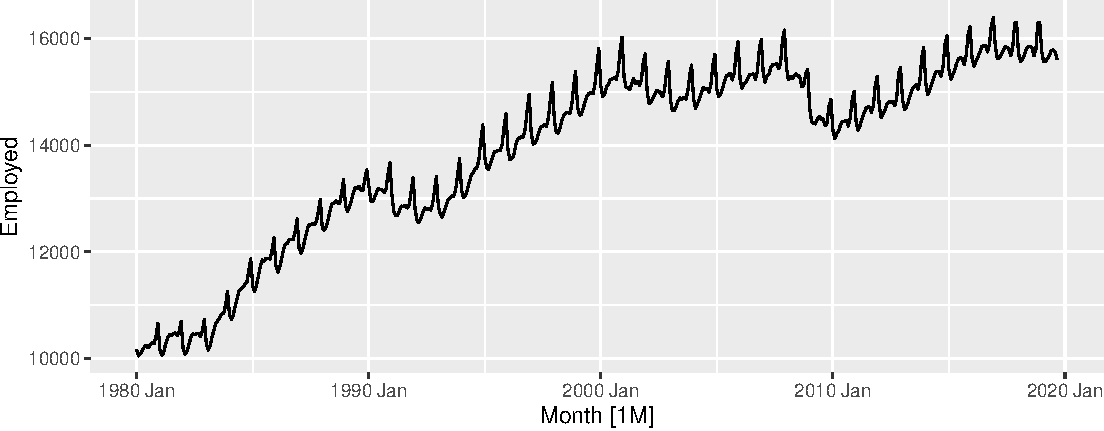
\includegraphics{2-tsgraphics_files/figure-beamer/unnamed-chunk-26-1.pdf}
\end{frame}

\begin{frame}[fragile]{US retail trade employment}
\protect\hypertarget{us-retail-trade-employment-1}{}
\fontsize{10}{10}\sf

\begin{Shaded}
\begin{Highlighting}[]
\NormalTok{retail }\SpecialCharTok{\%\textgreater{}\%}
  \FunctionTok{ACF}\NormalTok{(Employed, }\AttributeTok{lag\_max =} \DecValTok{48}\NormalTok{) }\SpecialCharTok{\%\textgreater{}\%}
  \FunctionTok{autoplot}\NormalTok{()}
\end{Highlighting}
\end{Shaded}

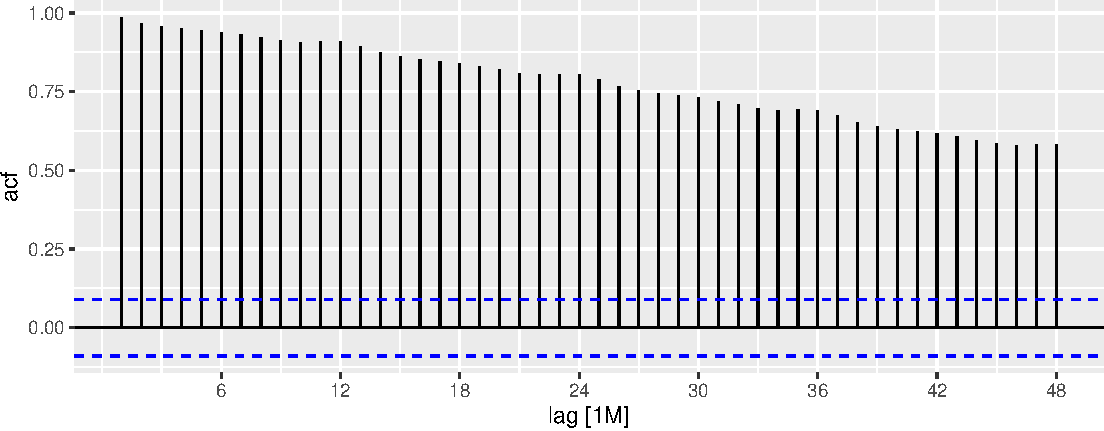
\includegraphics{2-tsgraphics_files/figure-beamer/unnamed-chunk-27-1.pdf}
\end{frame}

\begin{frame}[fragile]{Google stock price}
\protect\hypertarget{google-stock-price}{}
\fontsize{10}{10}\sf

\begin{Shaded}
\begin{Highlighting}[]
\NormalTok{google\_2015 }\OtherTok{\textless{}{-}}\NormalTok{ gafa\_stock }\SpecialCharTok{\%\textgreater{}\%}
  \FunctionTok{filter}\NormalTok{(Symbol }\SpecialCharTok{==} \StringTok{"GOOG"}\NormalTok{, }\FunctionTok{year}\NormalTok{(Date) }\SpecialCharTok{==} \DecValTok{2015}\NormalTok{) }\SpecialCharTok{\%\textgreater{}\%}
  \FunctionTok{select}\NormalTok{(Date, Close)}
\NormalTok{google\_2015}
\end{Highlighting}
\end{Shaded}

\begin{verbatim}
## # A tsibble: 252 x 2 [!]
##    Date       Close
##    <date>     <dbl>
##  1 2015-01-02  522.
##  2 2015-01-05  511.
##  3 2015-01-06  499.
##  4 2015-01-07  498.
##  5 2015-01-08  500.
##  6 2015-01-09  493.
##  7 2015-01-12  490.
##  8 2015-01-13  493.
##  9 2015-01-14  498.
## 10 2015-01-15  499.
## # ... with 242 more rows
## # i Use `print(n = ...)` to see more rows
\end{verbatim}
\end{frame}

\begin{frame}[fragile]{Google stock price}
\protect\hypertarget{google-stock-price-1}{}
\fontsize{10}{10}\sf

\begin{Shaded}
\begin{Highlighting}[]
\NormalTok{google\_2015 }\SpecialCharTok{\%\textgreater{}\%} \FunctionTok{autoplot}\NormalTok{(Close)}
\end{Highlighting}
\end{Shaded}

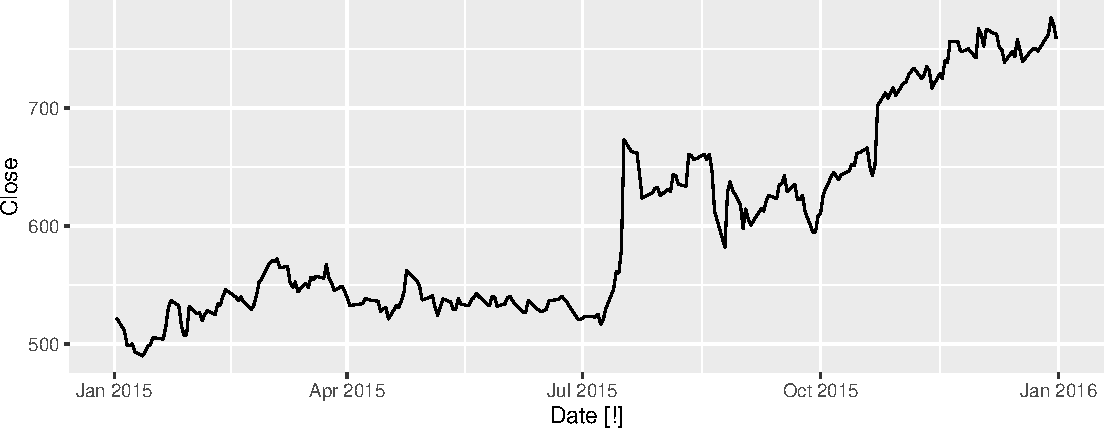
\includegraphics{2-tsgraphics_files/figure-beamer/unnamed-chunk-29-1.pdf}
\end{frame}

\begin{frame}[fragile]{Google stock price}
\protect\hypertarget{google-stock-price-2}{}
\fontsize{10}{10}\sf

\begin{Shaded}
\begin{Highlighting}[]
\NormalTok{google\_2015 }\SpecialCharTok{\%\textgreater{}\%}
  \FunctionTok{ACF}\NormalTok{(Close, }\AttributeTok{lag\_max=}\DecValTok{100}\NormalTok{)}
\end{Highlighting}
\end{Shaded}

\begin{verbatim}
## # A tsibble: 100 x 2 [1]
##      lag   acf
##    <lag> <dbl>
##  1     1 0.982
##  2     2 0.959
##  3     3 0.937
##  4     4 0.918
##  5     5 0.901
##  6     6 0.883
##  7     7 0.865
##  8     8 0.849
##  9     9 0.834
## 10    10 0.818
## # ... with 90 more rows
## # i Use `print(n = ...)` to see more rows
\end{verbatim}
\end{frame}

\begin{frame}[fragile]{Google stock price}
\protect\hypertarget{google-stock-price-3}{}
\fontsize{10}{10}\sf

\begin{Shaded}
\begin{Highlighting}[]
\NormalTok{google\_2015 }\SpecialCharTok{\%\textgreater{}\%}
  \FunctionTok{ACF}\NormalTok{(Close, }\AttributeTok{lag\_max =} \DecValTok{100}\NormalTok{) }\SpecialCharTok{\%\textgreater{}\%}
  \FunctionTok{autoplot}\NormalTok{()}
\end{Highlighting}
\end{Shaded}

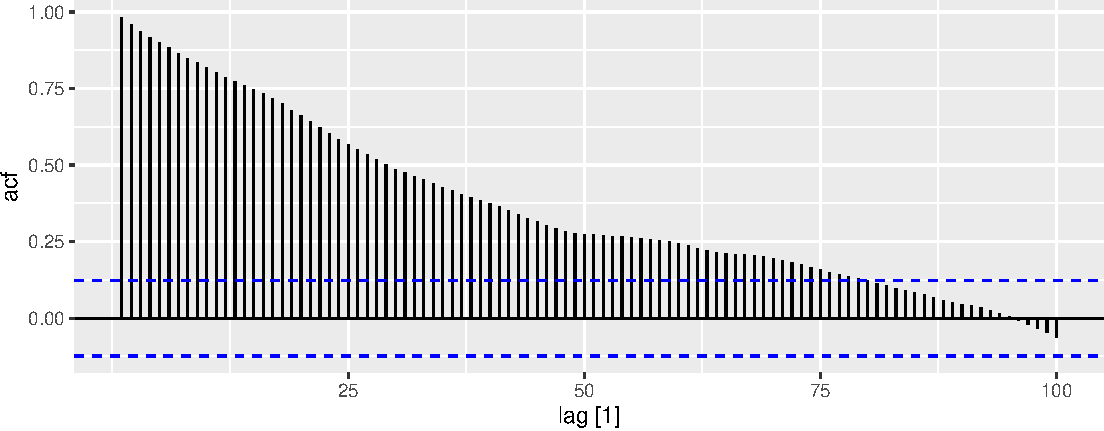
\includegraphics{2-tsgraphics_files/figure-beamer/unnamed-chunk-31-1.pdf}
\end{frame}

\begin{frame}{Which is which?}
\protect\hypertarget{which-is-which}{}
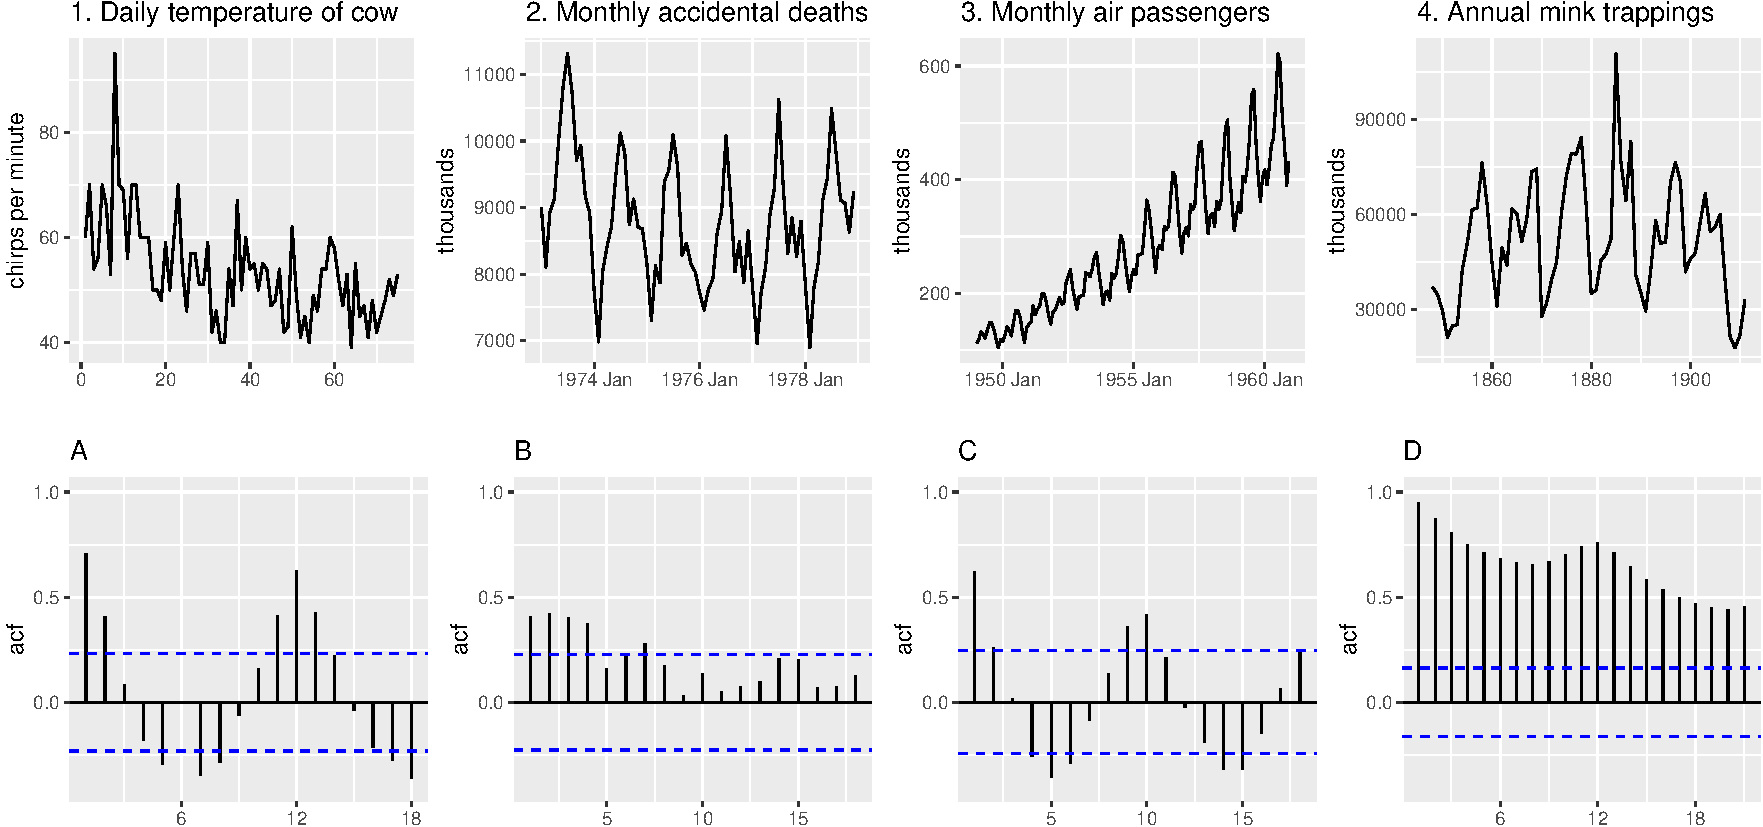
\includegraphics[width=15cm]{2-tsgraphics_files/figure-beamer/unnamed-chunk-32-1}
\end{frame}

\hypertarget{white-noise}{%
\section{White noise}\label{white-noise}}

\begin{frame}[fragile]{Example: White noise}
\protect\hypertarget{example-white-noise}{}
\fontsize{10}{10}\sf

\begin{Shaded}
\begin{Highlighting}[]
\FunctionTok{set.seed}\NormalTok{(}\DecValTok{30}\NormalTok{)}
\NormalTok{wn }\OtherTok{\textless{}{-}} \FunctionTok{tsibble}\NormalTok{(}\AttributeTok{t =} \DecValTok{1}\SpecialCharTok{:}\DecValTok{50}\NormalTok{, }\AttributeTok{y =} \FunctionTok{rnorm}\NormalTok{(}\DecValTok{50}\NormalTok{), }\AttributeTok{index =}\NormalTok{ t)}
\NormalTok{wn }\SpecialCharTok{\%\textgreater{}\%} \FunctionTok{autoplot}\NormalTok{(y)}
\end{Highlighting}
\end{Shaded}

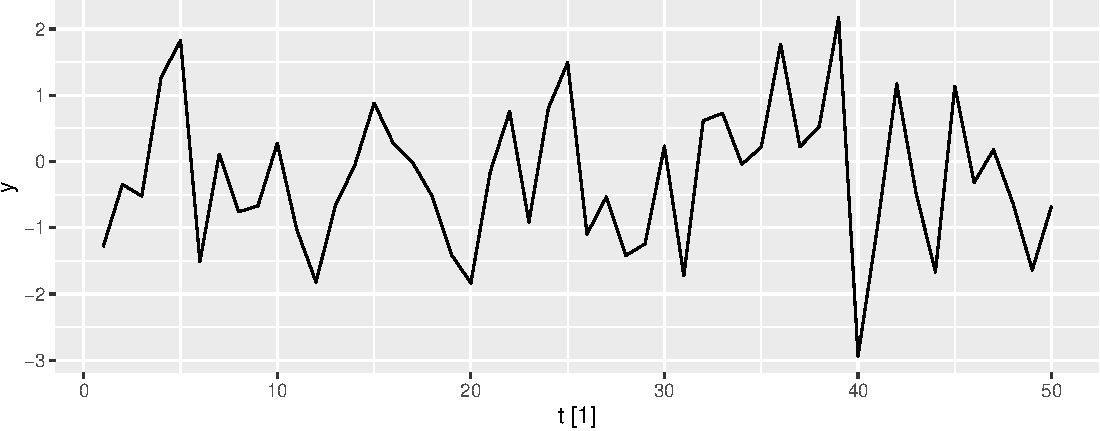
\includegraphics{2-tsgraphics_files/figure-beamer/wn-1.pdf}

\only<2>{
\begin{textblock}{10}(.4,6.6)\fontsize{12}{13}\sf
\begin{alertblock}{}
White noise data is uncorrelated across time with zero mean and constant variance.

(Technically, we require independence as well.)
\end{alertblock}
\end{textblock}}

\vspace*{10cm}
\end{frame}

\begin{frame}[fragile]{Example: White noise}
\protect\hypertarget{example-white-noise-1}{}
\fontsize{10}{10}\sf

\begin{Shaded}
\begin{Highlighting}[]
\NormalTok{wn }\SpecialCharTok{\%\textgreater{}\%} \FunctionTok{ACF}\NormalTok{(y)}
\end{Highlighting}
\end{Shaded}

\fontsize{10}{10}\sf\tabcolsep=0.1cm

\begin{longtable}[]{@{}
  >{\centering\arraybackslash}p{(\columnwidth - 18\tabcolsep) * \real{0.0989}}
  >{\centering\arraybackslash}p{(\columnwidth - 18\tabcolsep) * \real{0.0989}}
  >{\centering\arraybackslash}p{(\columnwidth - 18\tabcolsep) * \real{0.0989}}
  >{\centering\arraybackslash}p{(\columnwidth - 18\tabcolsep) * \real{0.0989}}
  >{\centering\arraybackslash}p{(\columnwidth - 18\tabcolsep) * \real{0.0989}}
  >{\centering\arraybackslash}p{(\columnwidth - 18\tabcolsep) * \real{0.0989}}
  >{\centering\arraybackslash}p{(\columnwidth - 18\tabcolsep) * \real{0.0989}}
  >{\centering\arraybackslash}p{(\columnwidth - 18\tabcolsep) * \real{0.0989}}
  >{\centering\arraybackslash}p{(\columnwidth - 18\tabcolsep) * \real{0.0989}}
  >{\centering\arraybackslash}p{(\columnwidth - 18\tabcolsep) * \real{0.1099}}@{}}
\toprule
\begin{minipage}[b]{\linewidth}\centering
\(r_{1}\)
\end{minipage} & \begin{minipage}[b]{\linewidth}\centering
\(r_{2}\)
\end{minipage} & \begin{minipage}[b]{\linewidth}\centering
\(r_{3}\)
\end{minipage} & \begin{minipage}[b]{\linewidth}\centering
\(r_{4}\)
\end{minipage} & \begin{minipage}[b]{\linewidth}\centering
\(r_{5}\)
\end{minipage} & \begin{minipage}[b]{\linewidth}\centering
\(r_{6}\)
\end{minipage} & \begin{minipage}[b]{\linewidth}\centering
\(r_{7}\)
\end{minipage} & \begin{minipage}[b]{\linewidth}\centering
\(r_{8}\)
\end{minipage} & \begin{minipage}[b]{\linewidth}\centering
\(r_{9}\)
\end{minipage} & \begin{minipage}[b]{\linewidth}\centering
\(r_{10}\)
\end{minipage} \\
\midrule
\endhead
0.014 & -0.163 & 0.163 & -0.259 & -0.198 & 0.064 & -0.139 & -0.032 &
0.199 & -0.024 \\
\bottomrule
\end{longtable}

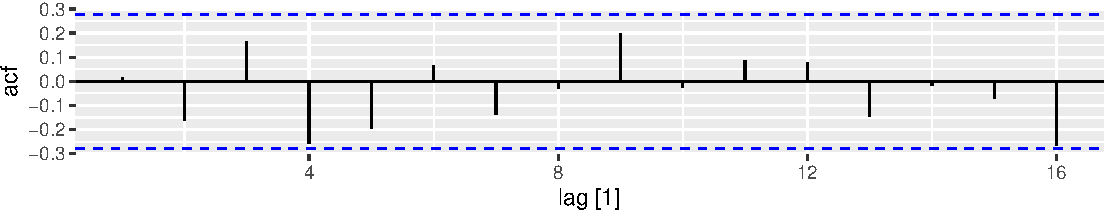
\includegraphics{2-tsgraphics_files/figure-beamer/unnamed-chunk-33-1.pdf}

\pause

\begin{itemize}
\tightlist
\item
  Sample autocorrelations for white noise series.
\item
  Expect each autocorrelation to be close to zero.
\item
  Blue lines show 95\% critical values.
\end{itemize}

\vspace*{10cm}
\end{frame}

\begin{frame}{\large Sampling distribution of autocorrelations}
\protect\hypertarget{sampling-distribution-of-autocorrelations}{}
Sampling distribution of \(r_k\) for white noise data is asymptotically
N(0,\(1/T\)).\pause

\begin{itemize}
\tightlist
\item
  95\% of all \(r_k\) for white noise must lie within
  \(\pm 1.96/\sqrt{T}\).
\item
  If this is not the case, the series is probably not WN.
\item
  Common to plot lines at \(\pm 1.96/\sqrt{T}\) when plotting ACF. These
  are the \alert{critical values}.
\end{itemize}
\end{frame}

\begin{frame}[fragile]{Example: Pigs slaughtered}
\protect\hypertarget{example-pigs-slaughtered}{}
\fontsize{10}{10}\sf

\begin{Shaded}
\begin{Highlighting}[]
\NormalTok{pigs }\OtherTok{\textless{}{-}}\NormalTok{ aus\_livestock }\SpecialCharTok{\%\textgreater{}\%}
  \FunctionTok{filter}\NormalTok{(State }\SpecialCharTok{==} \StringTok{"Victoria"}\NormalTok{, Animal }\SpecialCharTok{==} \StringTok{"Pigs"}\NormalTok{, }\FunctionTok{year}\NormalTok{(Month) }\SpecialCharTok{\textgreater{}=} \DecValTok{2014}\NormalTok{)}
\NormalTok{pigs }\SpecialCharTok{\%\textgreater{}\%} \FunctionTok{autoplot}\NormalTok{(Count}\SpecialCharTok{/}\FloatTok{1e3}\NormalTok{) }\SpecialCharTok{+}
  \FunctionTok{labs}\NormalTok{(}\AttributeTok{y =} \StringTok{"Thousands"}\NormalTok{, }\AttributeTok{title =} \StringTok{"Number of pigs slaughtered in Victoria"}\NormalTok{)}
\end{Highlighting}
\end{Shaded}

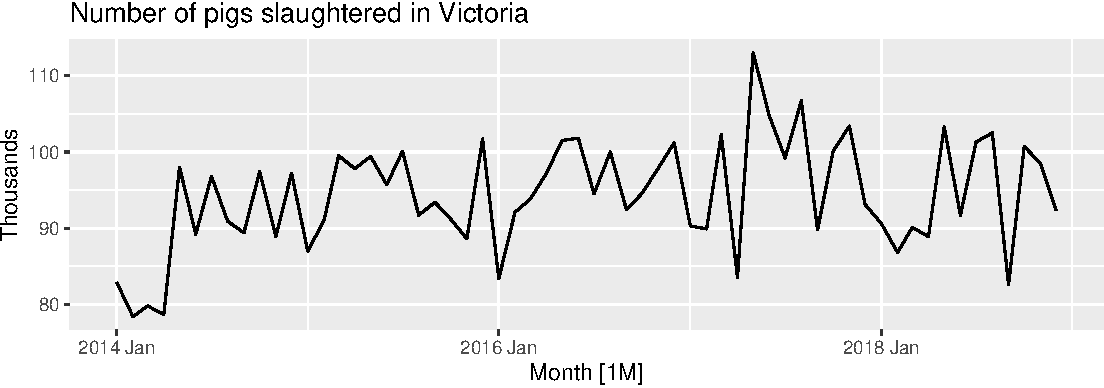
\includegraphics{2-tsgraphics_files/figure-beamer/unnamed-chunk-34-1.pdf}
\end{frame}

\begin{frame}[fragile]{Example: Pigs slaughtered}
\protect\hypertarget{example-pigs-slaughtered-1}{}
\fontsize{10}{10}\sf

\begin{Shaded}
\begin{Highlighting}[]
\NormalTok{pigs }\SpecialCharTok{\%\textgreater{}\%} \FunctionTok{ACF}\NormalTok{(Count) }\SpecialCharTok{\%\textgreater{}\%} \FunctionTok{autoplot}\NormalTok{()}
\end{Highlighting}
\end{Shaded}

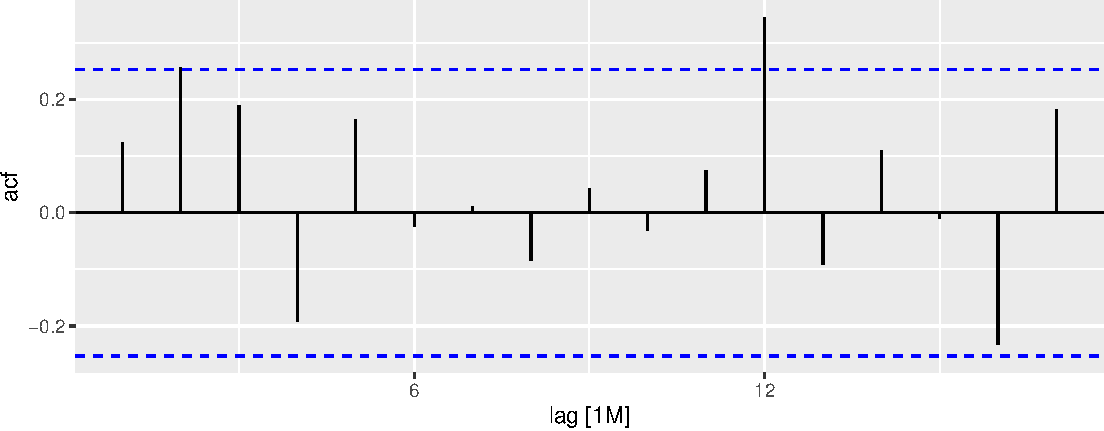
\includegraphics{2-tsgraphics_files/figure-beamer/unnamed-chunk-35-1.pdf}
\end{frame}

\begin{frame}{Example: Pigs slaughtered}
\protect\hypertarget{example-pigs-slaughtered-2}{}
Monthly total number of pigs slaughtered in the state of Victoria,
Australia, from January 2014 through December 2018 (Source: Australian
Bureau of Statistics.)\pause

\begin{itemize}
\tightlist
\item
  Difficult to detect pattern in time plot.
\item
  ACF shows significant autocorrelation for lag 2 and 12.
\item
  Indicate some slight seasonality.
\end{itemize}

\pause

These show the series is \textbf{not a white noise series}.
\end{frame}

\begin{frame}[fragile]{Your turn}
\protect\hypertarget{your-turn}{}
You can compute the daily changes in the Google stock price in 2018
using

\fontsize{11.5}{15}\sf

\begin{Shaded}
\begin{Highlighting}[]
\NormalTok{dgoog }\OtherTok{\textless{}{-}}\NormalTok{ gafa\_stock }\SpecialCharTok{\%\textgreater{}\%}
  \FunctionTok{filter}\NormalTok{(Symbol }\SpecialCharTok{==} \StringTok{"GOOG"}\NormalTok{, }\FunctionTok{year}\NormalTok{(Date) }\SpecialCharTok{\textgreater{}=} \DecValTok{2018}\NormalTok{) }\SpecialCharTok{\%\textgreater{}\%}
  \FunctionTok{mutate}\NormalTok{(}\AttributeTok{diff =} \FunctionTok{difference}\NormalTok{(Close))}
\end{Highlighting}
\end{Shaded}

\fontsize{14}{16}\sf

Does \texttt{diff} look like white noise?
\end{frame}

\begin{frame}[fragile]{2.10 Exercises (not an assignment but helpful!)}
\protect\hypertarget{exercises-not-an-assignment-but-helpful}{}
\begin{itemize}
\item
  Use help function: \texttt{?autoplot}
\item
  Try exercises that you are less familiar with
\end{itemize}
\end{frame}




\end{document}
